% =====================================================================
%  IGUALAB — DOCUMENTO DE ANÁLISIS Y DISEÑO
%  Versión LaTeX (reproducción del PDF "Análisis y Diseño - Igualab.pdf")
%  Compilar:  tectonic -X compile main.tex
% =====================================================================
\documentclass[11pt,a4paper]{article}

\usepackage{fontspec}
\usepackage[spanish,es-noindentfirst]{babel}
\usepackage[margin=2.54cm,top=2.54cm,bottom=2.54cm]{geometry}
\usepackage{xcolor}
\usepackage{graphicx}
\usepackage{array}
\usepackage{longtable}
\usepackage{tabularx}
\usepackage{colortbl}
\usepackage{makecell}
\usepackage{booktabs}
\usepackage{lscape}
\usepackage{fancyhdr}
\usepackage{titlesec}
\usepackage{titletoc}
\usepackage{tikz}
\usetikzlibrary{calc}
\usepackage{ragged2e}
\usepackage{enumitem}
\usepackage{parskip}
\usepackage{float}
\usepackage[hidelinks,colorlinks=true]{hyperref}
\usepackage{microtype}

% ---------------- Tipografías (equivalentes métricos de Arial) -------
\setmainfont{Liberation Sans}
\setsansfont{Liberation Sans}
\setmonofont{Liberation Mono}

% ---------------- Colores --------------------------------------------
\definecolor{linkblue}{HTML}{1155CC}
\definecolor{cellgray}{gray}{0.90}
\hypersetup{colorlinks=true,linkcolor=linkblue,urlcolor=linkblue,citecolor=linkblue}

% ---------------- Párrafos / interlineado ----------------------------
\setlength{\parindent}{0pt}
\setlength{\parskip}{7pt}
\linespread{1.15}
\renewcommand{\arraystretch}{1.35}

% ---- Opción B: texto JUSTIFICADO sin división de palabras (como Google Docs) ----
\hyphenpenalty=10000
\exhyphenpenalty=10000
\emergencystretch=3em
% Permitir corte solo en identificadores con guion bajo (p. ej. fragmentos_documento)
\let\igunderscore\_
\renewcommand{\_}{\igunderscore\allowbreak}

% ---------------- Encabezados ----------------------------------------
\titleformat{\section}
  {\normalfont\bfseries\fontsize{15.5}{18}\selectfont}
  {\thesection.}{0.7em}{\MakeUppercase}
\titlespacing*{\section}{0pt}{20pt}{8pt}

\titleformat{\subsection}
  {\normalfont\bfseries\fontsize{12.5}{15}\selectfont}
  {\thesubsection.}{0.6em}{}
\titlespacing*{\subsection}{0pt}{14pt}{6pt}

\titleformat{\subsubsection}
  {\normalfont\bfseries\normalsize}
  {\thesubsubsection.}{0.5em}{}
\titlespacing*{\subsubsection}{0pt}{10pt}{4pt}

% ---------------- Tablas ---------------------------------------------
\arrayrulecolor{black}
\setlength{\arrayrulewidth}{0.6pt}
\setlength{\tabcolsep}{4pt}
\setlength{\LTleft}{0pt}
\setlength{\LTright}{0pt}
\newcolumntype{L}[1]{>{\RaggedRight\arraybackslash}p{#1}}
\newcolumntype{C}[1]{>{\Centering\arraybackslash}p{#1}}
\newcommand{\thd}[1]{\textbf{#1}}

% ---------------- Encabezado de página -------------------------------
\pagestyle{fancy}
\fancyhf{}
\renewcommand{\headrulewidth}{0pt}
\fancyhead[L]{\small\thepage}

% Índice con puntos guía
\renewcommand{\contentsname}{Contenido}
\titlecontents{section}[2.4em]{\bfseries\vspace{3pt}}{\contentslabel{2.4em}}{}{\titlerule*[0.5pc]{.}\contentspage}
\titlecontents{subsection}[3.8em]{}{\contentslabel{2.2em}}{}{\titlerule*[0.5pc]{.}\contentspage}
\titlecontents{subsubsection}[5.4em]{}{\contentslabel{3.2em}}{}{\titlerule*[0.5pc]{.}\contentspage}

\setcounter{tocdepth}{3}
\setcounter{secnumdepth}{3}

% =====================================================================
\begin{document}

% -------------------------- PORTADA ---------------------------------
% ============================ PORTADA ===============================
\thispagestyle{empty}
\begin{tikzpicture}[remember picture, overlay]
  % Reglas negras (diseño de portada)
  \draw[line width=2.4pt] ($(current page.north west)+(10.62cm,-2.31cm)$)
        -- ($(current page.north west)+(10.62cm,-21.92cm)$);
  \draw[line width=2.4pt] ($(current page.north west)+(10.62cm,-2.31cm)$)
        -- ($(current page.north west)+(21cm,-2.31cm)$);
  \draw[line width=2.4pt] ($(current page.north west)+(10.62cm,-10.15cm)$)
        -- ($(current page.north west)+(21cm,-10.15cm)$);
  \draw[line width=2.4pt] ($(current page.north west)+(0cm,-18.35cm)$)
        -- ($(current page.north west)+(10.62cm,-18.35cm)$);

  % Logotipo
  \node at ($(current page.north west)+(15.95cm,-6.90cm)$)
    {
\includegraphics[width=8.80cm]{img/logo.png}};

  % Título
  \node[text width=9.80cm, align=center] at ($(current page.north west)+(15.95cm,-12.45cm)$)
    {\bfseries\fontsize{14}{17}\selectfont DOCUMENTO DE ANÁLISIS Y DISEÑO};
\end{tikzpicture}
\newpage


% -------------------- FRONT MATTER (numerada) -----------------------
% ===================== HISTORIAL DE VERSIONES ======================
\pagenumbering{arabic}
\thispagestyle{fancy}

\begin{center}
{\bfseries\fontsize{12}{14}\selectfont HISTORIAL DE VERSIONES}
\end{center}
\vspace{6pt}

\begin{center}
\begin{tabular}{|C{3.0cm}|C{2.2cm}|C{9.3cm}|}
\hline
\thd{FECHA} & \thd{VERSIÓN} & \thd{DESCRIPCIÓN} \\
\hline
03/09/2026 & V1 & Versión Inicial del documento \\
\hline
22/09/2026 & V2 & Versión final del documento \\
\hline
\end{tabular}
\end{center}

\vspace{16pt}

\begin{center}
\begingroup\small
\begin{tabular}{|C{1.6cm}|L{4.9cm}|L{4.6cm}|L{4.4cm}|}
\hline
 & \thd{AUTORES} & \thd{REVISADO POR} & \thd{APROBADO POR} \\
\hline
1.0 &
Luis Javier Millones Carrasco\newline
Carlos David Ordinola Ortega\newline
Fabricio Godofredo Ladera La Torre &
--- &
Elaboración de la primera versión del Documento de Análisis y Diseño \\
\hline
2.0 &
Fabricio Godofredo Ladera La Torre\newline
Luis Javier Millones Carrasco\newline
Carlos David Ordinola Ortega\newline
Juan Marcelo Ferreyra Gonzales\newline
Juan Renato Flores Pascual\newline
Mauricio Gabriel Gonzalez Kremer\newline
Alonso Aarón Benites Camacho &
Fabricio Godofredo Ladera La Torre\newline
Luis Javier Millones Carrasco\newline
Carlos David Ordinola Ortega\newline
Juan Marcelo Ferreyra Gonzales\newline
Mauricio Gabriel Gonzalez Kremer\newline
Alonso Aarón Benites Camacho &
Oscar Rafael Baldeón Montoro\newline
\emph{Cliente / Product Owner} \\
\hline
\end{tabular}
\endgroup
\end{center}

\vspace{18pt}

\noindent\textbf{Autores:}\\
\textbf{Project Manager:} Fabricio Godofredo Ladera La Torre\\
\textbf{Analista Funcional:} Luis Javier Millones Carrasco\\
\textbf{Analista Funcional:} Carlos David Ordinola Ortega\\
\textbf{Desarrollador backend:} Juan Marcelo Ferreyra Gonzales\\
\textbf{Desarrollador frontend:} Juan Renato Flores Pascual\\
\textbf{Analista de calidad:} Mauricio Gabriel Gonzalez Kremer\\
\textbf{Analista de calidad:} Alonso Aarón Benites Camacho

\vspace{10pt}

\noindent\textbf{Revisores:}\\
TCH: Teofilo Chambilla Aquino

\vspace{10pt}

\noindent\textbf{Aprobadores:}\\
Oscar Rafael Baldeón Montoro (Cliente / Product Owner)


% --------------------------- CONTENIDO ------------------------------
\clearpage
\phantomsection
{\centering\bfseries\fontsize{14}{17}\selectfont Contenido\par}
\vspace{10pt}
\makeatletter
\@starttoc{toc}
\makeatother

% ---------------------------- CUERPO --------------------------------
% ============================ GLOSARIO ==============================
\clearpage
\thispagestyle{fancy}
\begin{center}
{\bfseries\fontsize{14}{17}\selectfont GLOSARIO DE TÉRMINOS}
\end{center}
\vspace{10pt}

\newcommand{\glos}[2]{\par\vspace{4pt}\noindent\textbf{#1}: #2\par}
\newcommand{\grupo}[1]{\par\vspace{10pt}\noindent\textbf{\underline{#1}}\par\vspace{2pt}}
\glos{ASG (Ambiental, Social y Gobernanza)}{Dimensiones que evalúan el desempeño en sostenibilidad de una empresa.}
\glos{Brecha GRI}{Resultado de la revisión de un código GRI detectado en los documentos de una empresa cuya evidencia ha sido clasificada por el Administrador como Baja sustancia o Sub-reportado. El sistema identifica códigos y citas, pero no determina automáticamente el estado de la brecha.}
\glos{DEI / RSE}{Diversidad e Inclusión / Responsabilidad Social Empresarial, ámbitos de trabajo de Igualab.}
\glos{Estándar GRI (Global Reporting Initiative)}{Marco internacional de reportes de sostenibilidad, organizado en códigos por área temática (ej. GRI 400 = laboral/social).}
\glos{Memoria anual}{Documento financiero obligatorio para las empresas que cotizan en la Bolsa de Valores de Lima.}
\glos{Prospección comercial}{Identificación de empresas con brechas GRI o sanciones detectadas, para acercarse a ellas como aliado estratégico.}
\glos{Puntaje ESG}{Indicador numérico calculado automáticamente a partir de los estados asignados a los códigos GRI de una empresa (OK = 100, Baja sustancia = 50, Sub-reportado = 0).}
\glos{Reporte de sostenibilidad}{Documento anual de las empresas, auditado bajo el estándar GRI.}
\glos{Reporte de prospección}{Documento PDF generado por el sistema que consolida el estado de las brechas GRI, las sanciones identificadas y un resumen ejecutivo de una empresa, utilizado para el acercamiento comercial.}
\glos{Sanción económica}{Penalidad impuesta a una empresa, identificada exclusivamente a partir de menciones explícitas en los documentos ingestados.}
\glos{Sectores habilitados}{Los tres sectores acordados con el cliente para los cuales el sistema ejecuta el análisis de brechas: Minería, Petróleo y Gas, Energía.}

\glos{Administrador}{Rol operativo encargado de la explotación analítica del sistema: consulta al asistente de IA, revisión de brechas y sanciones, y generación de reportes de prospección.}
\glos{Auditoría}{Registro automático e inmutable de eventos sensibles del sistema (inicio de sesión, cambios de rol, ingesta, generación de reportes), consultable por el SuperAdmin.}
\glos{RBAC (Control de Accesos por Roles)}{Esquema que otorga permisos según el rol del usuario. En Igualab, el sistema reconoce únicamente dos roles: SuperAdmin y Administrador.}
\glos{SuperAdmin}{Rol con privilegios totales sobre la plataforma: gestiona usuarios y es responsable del catálogo de empresas y la ingesta de documentos fuente.}

\glos{Embedding}{Representación numérica (vector) de un fragmento de texto, generada por un modelo de IA, que permite medir la similitud semántica entre textos para habilitar la búsqueda del motor RAG.}
\glos{Hash SHA-256}{Algoritmo criptográfico utilizado para calcular una huella digital única de cada documento cargado, con el fin de detectar y rechazar duplicados.}
\glos{Ingesta}{Proceso de cargar al sistema las memorias anuales y reportes GRI, incluyendo su validación, indexación y disparo automático del análisis de brechas.}
\glos{JWT (JSON Web Token)}{Token firmado por el servidor que permite identificar a la cuenta y la sesión autenticada. El rol vigente no se obtiene exclusivamente del token, sino que se consulta en la base de datos en cada petición protegida.}
\glos{Markdown (.md)}{Formato de texto estructurado en el que deben ingresar los documentos fuente al sistema; el sistema no realiza conversión de formatos, por lo que el cliente entrega los documentos ya convertidos.}
\glos{Motor RAG (Retrieval-Augmented Generation)}{Componente de inteligencia artificial que responde consultas en lenguaje natural recuperando primero los fragmentos relevantes del corpus indexado, y generando luego una respuesta fundamentada exclusivamente en ellos.}
\glos{Estado OBSERVADO}{Estado que se asigna a un documento ingestado cuando no contiene ningún código GRI ni mención de sanción reconocible; el documento no se rechaza por completo, pero tampoco se indexa hasta corregirse.}

\glos{Análisis GAP (AS IS / TO BE)}{Comparación entre la situación actual del proceso (manual) y la situación objetivo (con el sistema implementado).}
\glos{Definition of Done (DoD)}{Criterios que un incremento debe cumplir para considerarse terminado.}
\glos{MVP (Producto Mínimo Viable)}{Versión inicial del sistema con las funcionalidades esenciales para validar el valor con el cliente.}
\glos{Product Backlog}{Lista priorizada de todos los requerimientos del producto.}
\glos{Sprint}{Iteración de trabajo de duración fija en la que se produce un incremento del producto.}
\glos{Sprint Backlog}{Conjunto de historias y tareas comprometidas para el sprint.}
\glos{UAT (Prueba de Aceptación de Usuario)}{Validación final del sistema realizada por el cliente antes de la entrega.}

\glos{Caso de Uso (CU)}{Descripción estructurada de una interacción entre un actor y el sistema para lograr un objetivo específico (ej. CU003: Ingesta de Documentos).}
\glos{Regla de Negocio (RN)}{Política o condición del dominio que el sistema debe respetar, referenciada por uno o varios requerimientos funcionales.}
\glos{Requerimiento Funcional (RF)}{Descripción de una función concreta y verificable que el sistema debe ejecutar.}
\glos{Requerimiento No Funcional (RNF)}{Atributo de calidad, seguridad o rendimiento que el sistema debe cumplir de forma transversal (ej. tiempo de respuesta, cifrado).}


\clearpage
% ====================================================================
%  SECCIONES 1–6
% ====================================================================

\section{Antecedentes}
Igualab es una organización peruana dedicada a la consultoría en Diversidad e Inclusión (DEI), sostenibilidad y Responsabilidad Social Empresarial (RSE), enfocada en promover entornos laborales inclusivos y prácticas ASG (Ambiental, Social y Gobernanza) en el sector empresarial peruano. Fundada en 2016, cuenta con certificaciones como Entidad Perceptora de Donaciones (EPD) y reconocimientos internacionales como el Corporate Live Wire Innovation \& Excellence Awards.

En el contexto peruano, las empresas que cotizan en la Bolsa de Valores de Lima (BVL) ---del orden de 115 emisores--- están obligadas a emitir memorias anuales financieras, mientras que los reportes de sostenibilidad son validados por auditores internacionales bajo estándares como el GRI (Global Reporting Initiative). Estos documentos contienen información crítica sobre cumplimiento normativo, sanciones económicas, indicadores de gobernanza y métricas de desempeño ambiental y social.

\textbf{Problemática.} Hoy Igualab opera de manera reactiva en su área comercial: recibe empresas de forma orgánica y no cuenta con herramientas que sistematicen el análisis de la información pública para detectar oportunidades de acercamiento. Buscar, leer y comparar manualmente memorias y reportes (que suelen exceder las 100 páginas) es lento, no es trazable y no escala al universo de emisores de la BVL.

Frente a ello, se plantea el desarrollo de una plataforma web basada en inteligencia artificial (RAG) que permita procesar reportes de sostenibilidad y memorias anuales, identificar brechas en indicadores ASG/GRI y generar información procesada que facilite la toma de decisiones comerciales.

\section{Objetivo General}
Desarrollar una plataforma web de analítica de sostenibilidad que permita a Igualab procesar y consultar información pública de empresas (reportes de sostenibilidad y memorias anuales de la Bolsa de Valores de Lima), identificando brechas en indicadores ASG mediante un asistente de inteligencia artificial (RAG), para impulsar la prospección comercial de la organización de manera proactiva y fundamentada en datos.

\subsection{Objetivos específicos}
\begin{enumerate}[leftmargin=1.6em,itemsep=4pt,topsep=4pt]
  \item Diseñar la arquitectura de la plataforma que integre la información pública de las empresas (memorias anuales y reportes de sostenibilidad) y habilite su explotación mediante inteligencia artificial, asegurando escalabilidad, confiabilidad y eficiencia en el uso de recursos.
  \item Implementar la autenticación y el control de acceso por roles (RBAC) con dos perfiles ---SuperAdmin (gestión) y Administrador (explotación analítica)---, garantizando la seguridad y la trazabilidad de las operaciones.
  \item Desarrollar el módulo de ingesta que permita al SuperAdmin cargar documentos en Markdown (.md) y los deje indexados para su consulta por el Administrador a través de la inteligencia artificial.
  \item Implementar el asistente de inteligencia artificial (RAG) que permita al Administrador consultar en lenguaje natural los documentos ingestados, apoyando la identificación de brechas en códigos GRI y de sanciones económicas, y citando siempre la fuente de la información.
  \item Desarrollar la generación de reportes de prospección en formato PDF a partir de las brechas GRI y sanciones ya validadas, incluyendo un resumen ejecutivo y el puntaje ESG.
  \item Establecer el sistema de auditoría que registre los eventos sensibles (inicios de sesión, cambios de rol, ingesta de datos y generación de reportes) para garantizar la trazabilidad y el cumplimiento de las políticas de seguridad.
\end{enumerate}

\section{Alcance del Proyecto}
El proyecto comprende el diseño, desarrollo e implementación de una plataforma web que centralice la ingesta, indexación, consulta y explotación analítica de memorias anuales y reportes de sostenibilidad (GRI) de empresas que cotizan en la Bolsa de Valores de Lima (BVL), mediante una arquitectura cliente-servidor y un motor de inteligencia artificial basado en RAG (Retrieval-Augmented Generation). Este documento detalla el alcance de la \textbf{FASE 1} (primera versión del software).

\subsection{Roles del sistema}
El sistema está orientado a optimizar las operaciones de dos perfiles (acta CS3081-004-2026 · REQ-10):

\begin{itemize}[leftmargin=1.4em,itemsep=2pt,topsep=2pt]
  \item \textbf{SuperAdmin (1 persona):} gestiona las cuentas de la plataforma (creación, habilitación y deshabilitación, y transferencia del rol) y es responsable del catálogo de empresas y de la ingesta de documentos de sostenibilidad y memorias anuales al sistema.
  \item \textbf{Administrador (2 personas):} realiza consultas al asistente de inteligencia artificial (RAG), revisa y valida las brechas GRI y sanciones, y genera reportes de prospección comercial en formato PDF.
\end{itemize}

El SuperAdmin concentra tanto la administración de accesos como la carga de información fuente, mientras que el Administrador se enfoca exclusivamente en la explotación analítica y comercial de dicha información.

\subsection{Sectores en alcance}
Por acuerdo con el cliente, el análisis de brechas GRI y sanciones se limita a tres sectores: \textbf{Minería, Petróleo y Gas, y Energía} (acta CS3081-003-2026 · REQ-07). Las empresas de otros sectores quedan fuera del análisis y de la generación de reportes en la FASE 1.

\subsection{Fuera de alcance de la FASE 1}
Se declaran explícitamente fuera del alcance de la FASE 1 las siguientes funcionalidades, por decisión del cliente registrada en acta:

\begin{center}
\begin{tabular}{|L{5.4cm}|L{9.6cm}|}
\hline
\thd{Excluido de la FASE 1} & \thd{Referencia (acta)} \\
\hline
Módulo de la Bolsa de Valores (y sus CU/RF asociados) & acta CS3081-005-2026 · REQ-16 \\
\hline
Búsqueda de contactos vía LinkedIn & acta CS3081-005-2026 · REQ-17 \\
\hline
Dashboards de visualización (KPIs ASG/ESG) & acta CS3081-005-2026 · REQ-19 \\
\hline
Portal público y chatbot/asistente vocal & actas CS3081-001 y 002 (FASE 2) \\
\hline
Usuarios ``Cliente'' (multi-tenant) y pasarela de pagos & acta CS3081-004-2026 · REQ-12 \\
\hline
Despliegue a producción (operación en el entorno universitario) & acta CS3081-004-2026 · REQ-11 \\
\hline
\end{tabular}
\end{center}

\subsection{Nota de terminología}
En este documento, \textbf{FASE 1} y \textbf{FASE 2} designan \textbf{versiones del software} (FASE 1 = primera versión, la que aquí se detalla; FASE 2 = versión futura). No deben confundirse con las \textbf{cuatro fases de desarrollo} del Plan de Proyecto v1.2 (Inicial, Análisis y Diseño, Desarrollo, Cierre), que describen la metodología de ejecución del proyecto.

% --------------------------------------------------------------------
\section{Diseño Funcional Detallado}
La solución consiste en una plataforma web de analítica de sostenibilidad que permite a Igualab procesar reportes de sostenibilidad y memorias anuales de empresas que cotizan en la Bolsa de Valores de Lima, identificar brechas en indicadores ASG mediante inteligencia artificial y generar reportes de prospección comercial. La plataforma se estructura como un \textbf{monolito modular} sobre dos roles ---SuperAdmin y Administrador---, organizado en \textbf{ocho módulos funcionales} y un componente transversal de configuración.

\subsection{Criterios de diseño y modularización}
Conforme a los fundamentos de diseño ---modularidad, abstracción, acoplamiento y cohesión--- y a los principios \textbf{SOLID}, el sistema se descompone en módulos de grano fino y responsabilidad única:

\begin{itemize}[leftmargin=1.4em,itemsep=2pt,topsep=2pt]
  \item \textbf{Modularidad:} cada módulo agrupa una responsabilidad funcional y puede evolucionar y probarse de forma independiente.
  \item \textbf{Abstracción:} los servicios exponen interfaces estables y ocultan los detalles de implementación (proveedor de IA, almacenamiento, correo).
  \item \textbf{Alta cohesión y bajo acoplamiento:} cada módulo es dueño único de sus datos y se comunica mediante interfaces bien definidas.
  \item \textbf{Aplicación de SOLID en Igualab:} cada módulo se implementa con un único servicio de responsabilidad única y su propio conjunto de datos; las integraciones externas (proveedor de IA y servicio de correo) se resuelven mediante interfaces sustituibles; cada servicio expone solo las operaciones que su consumidor requiere; y la configuración se inyecta por variables de entorno, no desde implementaciones concretas. En concreto:
    \begin{itemize}[leftmargin=1.2em,itemsep=2pt,topsep=2pt]
      \item \emph{Responsabilidad única:} un servicio por módulo (\texttt{auth\_service}, \texttt{ingesta\_service}, \texttt{gri\_analisis\_service}, \texttt{rag\_chat\_service}, \texttt{reportes\_pdf\_service}, \texttt{auditoria\_service}); la autenticación no se mezcla con la ingesta ni con los reportes.
      \item \emph{Abierto/cerrado:} cambiar de proveedor de IA o de correo no obliga a modificar los servicios, porque se accede a ellos por interfaz.
      \item \emph{Sustitución:} las implementaciones de \texttt{LlmClient} y \texttt{EmbeddingClient} (proveedor \emph{free} y respaldo) son intercambiables sin tocar el código que las consume.
      \item \emph{Segregación de interfaces:} cada módulo publica únicamente las operaciones que su consumidor necesita (por ejemplo, la auditoría es de solo lectura para el SuperAdmin).
      \item \emph{Inversión de dependencias:} los servicios dependen de abstracciones (repositorios y cliente de IA) y la configuración entra por variables de entorno (\texttt{LLM\_*}, \texttt{EMBEDDING\_*}, \texttt{UPLOAD\_MAX\_MB}).
    \end{itemize}
\end{itemize}

\noindent\textbf{Decisión de despliegue:} la FASE 1 se implementa como un monolito modular (una sola unidad desplegable, con los módulos separados internamente); no se adoptan microservicios en esta versión.

\subsection{Catálogo de módulos funcionales}
Cada módulo indica el servicio que lo implementa (SRP), su caso de uso y los requisitos que cubre.

\begin{center}
\begingroup\small
\begin{longtable}{|C{0.7cm}|L{4.4cm}|C{1.4cm}|L{7.8cm}|}
\hline
\thd{\#} & \thd{Módulo / Servicio (SRP)} & \thd{CU} & \thd{Requisitos (RF · RN · RNF)} \\
\hline
\endhead
1 & Autenticación y Gestión de Sesión --- \texttt{auth\_service} & CU001 & RN-001…RN-013 · RF-001…RF-005 · RNF-001…RNF-009 \\
\hline
2 & Gestión de Usuarios --- \texttt{usuario\_service} & CU002 & RN-001…RN-009 · RF-006…RF-009 · RNF-012, RNF-013 \\
\hline
3 & Catálogo de Empresas --- \texttt{empresa\_service} & CU003 & RN-014…RN-017 · RF-010, RF-011 · --- \\
\hline
4 & Ingesta de Documentos --- \texttt{ingesta\_service} & CU003 & RN-018…RN-026 · RF-012…RF-017 · RNF-007, RNF-011, RNF-015, RNF-016, RNF-020, RNF-025, RNF-029, RNF-031 \\
\hline
5 & Análisis y Validación de Brechas GRI --- \texttt{gri\_analisis\_service} & CU005 & RN-027…RN-032 · RF-018…RF-022, RF-027 · RNF-014, RNF-026, RNF-027 \\
\hline
6 & Asistente de IA (RAG) --- \texttt{rag\_chat\_service} & CU004 & RN-033…RN-037 · RF-023, RF-024 · RNF-010, RNF-017, RNF-018, RNF-019 \\
\hline
7 & Generación de Reportes de Prospección --- \texttt{reportes\_pdf\_service} & CU006 & RN-038…RN-041 · RF-025, RF-026 · --- \\
\hline
8 & Auditoría Funcional --- \texttt{auditoria\_service} & CU007 & RN-042…RN-045 · RF-028 · RNF-022, RNF-023, RNF-024 \\
\hline
--- & Configuración (transversal, sin módulo propio) & --- & Parámetros por variables de entorno: tamaño máximo de ingesta y cuota del proveedor de IA (RNF-020, RNF-027) \\
\hline
\end{longtable}
\endgroup
\end{center}

\noindent{\small La numeración de CU y de requisitos corresponde a la del presente documento (secciones 6 y 7).}

\subsection{Descripción de los módulos}

\subsubsection{Módulo 1 --- Autenticación y Gestión de Sesión}
Controla el acceso a la plataforma mediante correo y contraseña, garantizando que solo cuentas registradas y habilitadas puedan operar el sistema. Contempla la recuperación de contraseña por enlace temporal de un solo uso, el cambio de contraseña estando autenticado, la expiración de sesión por inactividad, el cierre de sesión manual y el bloqueo temporal de la cuenta tras 5 intentos fallidos consecutivos. La sesión se soporta con un token JWT firmado que incorpora la identidad de la cuenta, mientras que el rol vigente se valida en cada petición.

\subsubsection{Módulo 2 --- Gestión de Usuarios}
Exclusivo del SuperAdmin: permite crear cuentas de Administrador (con contraseña temporal para el primer acceso), habilitarlas o deshabilitarlas ---invalidando de inmediato sus sesiones activas--- y transferir el rol SuperAdmin a una cuenta de Administrador existente y habilitada, con confirmación previa y ejecución atómica. El sistema garantiza en todo momento la existencia de exactamente una cuenta con rol SuperAdmin y no contempla eliminación permanente de cuentas, solo habilitación y deshabilitación, para preservar la trazabilidad de auditoría.

\subsubsection{Módulo 3 --- Catálogo de Empresas}
Exclusivo del SuperAdmin: registra las empresas sobre las cuales se realizará el análisis, exigiendo nombre y sector. El sector es un atributo de la empresa y pertenece a un conjunto cerrado de tres valores (Minería, Petróleo y Gas, y Energía); las empresas de otros sectores no son elegibles para el análisis ni para la generación de reportes.

\subsubsection{Módulo 4 --- Ingesta de Documentos}
Exclusivo del SuperAdmin: carga memorias anuales y reportes de sostenibilidad GRI en formato Markdown (.md), asociados obligatoriamente a una empresa, un año y un tipo de documento. El sistema valida el tipo real del archivo en el servidor, calcula su hash SHA-256 para rechazar duplicados y verifica que contenga al menos un código GRI o una mención de sanción reconocible; en caso contrario, el documento se marca como observado en lugar de rechazarse por completo. El procesamiento es síncrono, con progreso visible al usuario, e incluye la indexación del contenido y la ejecución automática del análisis de brechas GRI como último paso de una ingesta exitosa. Ante rechazo o interrupción, el sistema revierte el procesamiento sin conservar contenido parcial.

\subsubsection{Módulo 5 --- Análisis y Validación de Brechas GRI}
Exclusivo del Administrador: traduce el contenido indexado en un diagnóstico de cumplimiento GRI con supervisión humana obligatoria. El motor identifica automáticamente qué códigos del catálogo GRI (40 códigos) están presentes en el documento, citando el fragmento de origen, sin comparar contra el texto del estándar GRI oficial. El Administrador revisa cada cita textual y asigna manualmente el estado del código (OK, Baja sustancia o Sub-reportado); el sistema no infiere ni calcula este estado de forma automática. Las sanciones económicas se identifican exclusivamente a partir de menciones explícitas en los documentos ingestados. El puntaje ESG se calcula a partir de los estados asignados; si no se detectó ningún código, se muestra como ``no disponible'', nunca como cero.

\subsubsection{Módulo 6 --- Asistente de Inteligencia Artificial (RAG)}
Exclusivo del Administrador: permite consultas en lenguaje natural sobre el corpus indexado, requiriendo seleccionar sector, empresa y año antes de habilitar la consulta. El asistente se limita a responder sobre sostenibilidad empresarial, indicadores GRI, sanciones o el contenido de los documentos ingestados; ante cualquier otra consulta declina explícitamente. Toda respuesta incluye la referencia al documento, empresa y año de origen, y suprime cualquier afirmación sin fuente verificable en el corpus; ante información insuficiente, lo declara en lugar de inventar una respuesta. El contenido recuperado se trata siempre como datos de referencia dentro del prompt, nunca como instrucciones del sistema. Ante indisponibilidad del proveedor externo de IA, informa el error sin bloquear el resto de los módulos.

\subsubsection{Módulo 7 --- Generación de Reportes de Prospección}
Exclusivo del Administrador: consolida el análisis validado de una empresa en un documento PDF para el acercamiento comercial. Solo puede generarse para empresas con al menos un documento indexado y se construye exclusivamente a partir de los resultados de análisis ya almacenados y validados manualmente, sin invocar al servicio de IA en este paso, por lo que dos generaciones sobre los mismos datos producen el mismo resultado. El reporte incluye el estado de cada código GRI con su cita de respaldo, las sanciones identificadas (con monto o marcadas como ``no cuantificada'') y un resumen ejecutivo con el puntaje ESG. Una vez generado, el reporte es inmutable; su historial es visualizable y descargable por cualquier Administrador.

\subsubsection{Módulo 8 --- Auditoría Funcional}
Exclusivo del SuperAdmin: registra automáticamente todo evento sensible del sistema ---inicio de sesión, cambio de estado o rol de cuenta, ingesta, rechazo de documento y generación de reportes---, consignando la cuenta responsable, la fecha y hora (UTC) y el tipo de acción. El registro es consultable filtrando por usuario, fecha y tipo de evento, y es de solo inserción: no admite edición ni eliminación.

\subsection{Flujos funcionales end-to-end}
\begin{itemize}[leftmargin=1.4em,itemsep=3pt,topsep=2pt]
  \item \textbf{F1 · Ingesta y análisis (SuperAdmin):} autenticarse $\rightarrow$ seleccionar sector y empresa, año y tipo $\rightarrow$ subir el \texttt{.md} $\rightarrow$ \emph{guard} (extensión, tamaño, hash) $\rightarrow$ parseo y chunking $\rightarrow$ \emph{embeddings} por API $\rightarrow$ indexación $\rightarrow$ detección de códigos GRI y sanciones (filas sin estado) $\rightarrow$ auditoría $\rightarrow$ resultado con progreso.
  \item \textbf{F2 · Consulta RAG (Administrador):} seleccionar sector, empresa y año $\rightarrow$ formular la pregunta $\rightarrow$ recuperación semántica $\rightarrow$ respuesta del modelo con citas (o declinación fuera de dominio).
  \item \textbf{F3 · Revisión de brechas (Administrador):} abrir las filas con su cita $\rightarrow$ asignar el estado manual $\rightarrow$ registrar el histórico.
  \item \textbf{F4 · Reporte de prospección (Administrador):} verificar estados validados $\rightarrow$ generar el PDF determinista (sin IA) $\rightarrow$ snapshot inmutable $\rightarrow$ auditoría $\rightarrow$ historial y descarga.
  \item \textbf{F5 · Autenticación y usuarios (SuperAdmin):} iniciar sesión o recuperar contraseña; crear, habilitar/deshabilitar y transferir el rol SuperAdmin (atómico).
  \item \textbf{F6 · Auditoría (SuperAdmin):} consultar y filtrar los eventos; solo lectura.
\end{itemize}

\subsection{Reglas transversales de diseño}
\begin{enumerate}[leftmargin=1.6em,itemsep=2pt,topsep=2pt]
  \item \textbf{RBAC de dos roles} en cada endpoint (autorización por petición; el rol se valida en el servidor).
  \item \textbf{Ingesta síncrona} de \texttt{.md} (tablas con pipes), con hash y \textbf{reversión atómica} ante fallo.
  \item \textbf{Tres estados GRI}, asignación 100\,\% manual; el puntaje ESG se deriva y es ``no disponible'' si no hay códigos.
  \item \textbf{RAG simple} sin \emph{function calling}; citación obligatoria; el corpus se trata como datos (anti \emph{prompt injection}); \emph{timeout} de IA de 1 minuto.
  \item \textbf{Reporte determinista sin IA} e inmutable.
  \item \textbf{Auditoría append-only} en UTC.
  \item \textbf{Trazabilidad:} cada módulo referencia sus CU $\leftrightarrow$ RF $\leftrightarrow$ RN $\leftrightarrow$ RNF (tabla anterior).
\end{enumerate}

% --------------------------------------------------------------------
\section{Diagrama del Proceso}
En este apartado se presentan los diagramas del proceso: la integración entre los sistemas de la empresa en la situación actual (5.1) y la interoperación con los sistemas externos vinculados con ella en la situación propuesta (5.2).

\subsection{Integración entre los sistemas de la empresa}
En la situación actual (AS-IS), Igualab no integra sistemas para el análisis comercial: el analista realiza todo el proceso de forma manual y reactiva. Busca y descarga cada informe (memoria anual y/o reporte de sostenibilidad) de fuentes dispersas, lo lee íntegramente, identifica brechas, sanciones y oportunidades de mejora, y elabora el documento de prospección en texto libre. No existe una base de datos ni una aplicación que articule estas actividades, por lo que no hay trazabilidad, comparación entre empresas ni reutilización de resultados. La figura siguiente representa el flujo end-to-end actual.

\begin{center}
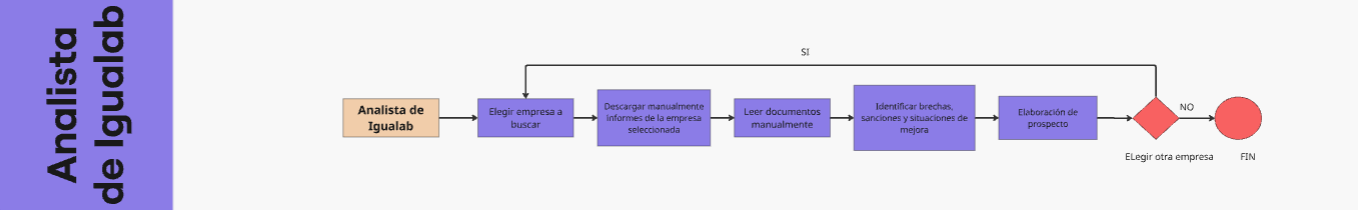
\includegraphics[width=0.94\textwidth]{img/im-011-009.png}
\end{center}

\subsection{Interoperación con sistemas externos vinculados con la empresa}
En la situación propuesta (TO-BE), la plataforma articula internamente el proceso y se comunica con sistemas externos mediante interfaces estandarizadas: el \textbf{proveedor de IA} (embeddings y generación por HTTPS/JSON), el \textbf{servicio de correo} (SMTP, para la recuperación de contraseña) y la \textbf{Bolsa de Valores de Lima (BVL)}, que es la fuente de los documentos y que el cliente entrega ya convertidos a Markdown, sin integración por API. El asistente de IA consume al proveedor externo como un servicio, sin que el modelo decida acciones sobre el sistema, y el contenido recuperado del corpus se trata como datos, nunca como instrucciones. Con ello, el proceso se organiza en los carriles del Sistema (automático), el SuperAdmin (gestión e ingesta) y el Administrador (explotación analítica), e incorpora el análisis GRI y de sanciones y la generación del reporte. La figura siguiente representa el proceso objetivo.

\begin{center}
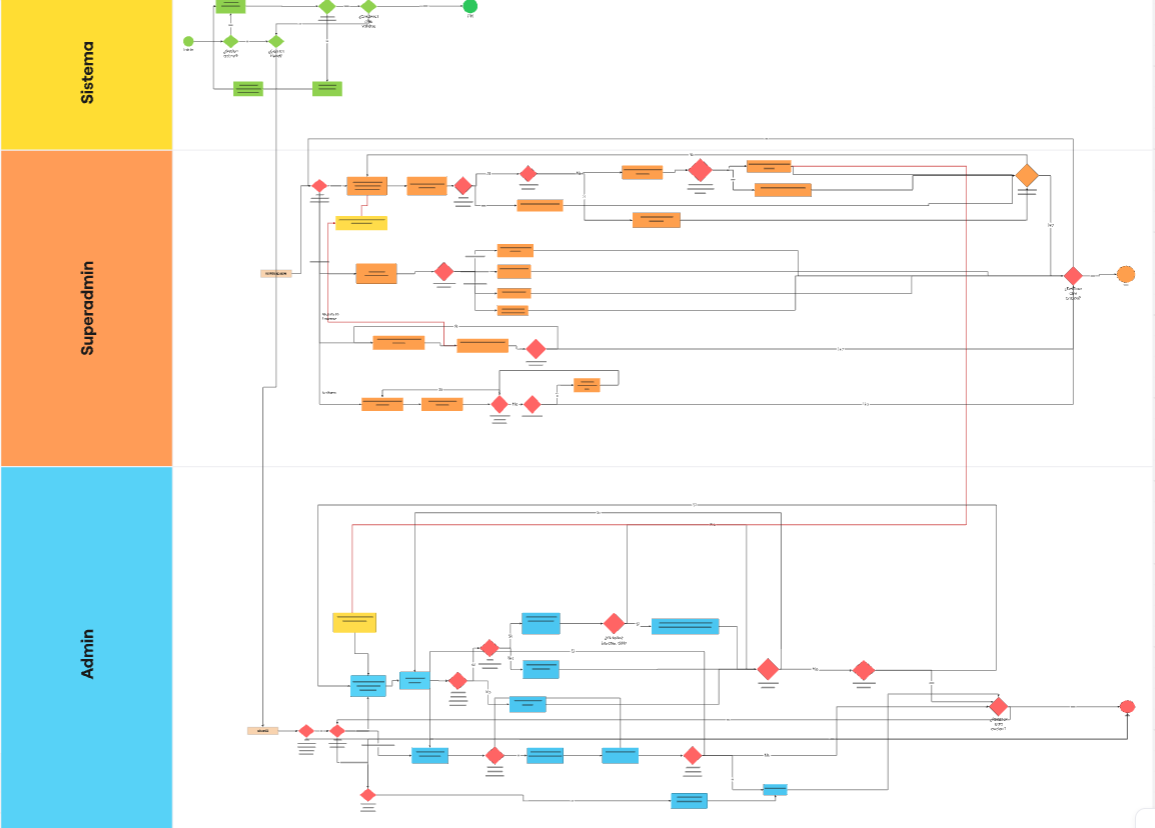
\includegraphics[width=0.96\textwidth]{img/im-012-010.png}
\end{center}
\noindent Enlace del tablero del proceso: \href{https://miro.com/app/board/uXjVHq4p518=/}{https://miro.com/app/board/uXjVHq4p518=/}

% --------------------------------------------------------------------
\section{Reglas de Negocio}
Las Reglas de Negocio (RN) se detallan a continuación, agrupadas por dominio: acceso y cuentas, empresas y sectores, ingesta documental, análisis GRI, asistente IA, reportes de prospección y auditoría.

\begingroup\small
\begin{longtable}{|C{1.4cm}|L{4.0cm}|L{9.4cm}|}
\hline
\thd{RN} & \thd{NOMBRE DE LA REGLA} & \thd{DETALLE DE LA REGLA} \\
\hline
RN-001 & Conjunto cerrado de roles & \textbf{SI} una cuenta opera en la plataforma, \textbf{ENTONCES} el sistema le reconoce exactamente uno de dos roles ---SuperAdmin o Administrador--- y aplica únicamente los permisos de ese rol. \textbf{SE APLICA A} todas las cuentas y a todos los módulos y endpoints de la plataforma. \textbf{SE BASA EN} el modelo RBAC de dos roles acordado con el cliente (acta CS3081-004-2026 · REQ-10) y en el principio de mínimo privilegio. \textbf{Y TIENE LA SIGUIENTE EXCEPCIÓN} no se admiten roles adicionales (p. ej. «Usuario») ni cuentas sin rol asignado. \\
\hline
RN-002 & Unicidad del SuperAdmin & \textbf{SI} se crea, habilita, deshabilita o transfiere una cuenta, \textbf{ENTONCES} el sistema garantiza que exista exactamente una cuenta con rol SuperAdmin en todo momento, con independencia de su estado de habilitación o de si mantiene una sesión abierta. \textbf{SE APLICA A} la creación de cuentas, la habilitación/deshabilitación y la transferencia de rol. \textbf{SE BASA EN} el principio de responsabilidad única sobre la administración del sistema y en el acuerdo del cliente (acta CS3081-004-2026 · REQ-10). \textbf{Y TIENE LA SIGUIENTE EXCEPCIÓN} la cuenta SuperAdmin inicial se crea durante el despliegue y no puede crearse desde la aplicación (RN-006). \\
\hline
RN-003 & Permisos cerrados por rol & \textbf{SI} una cuenta intenta ejecutar una acción, \textbf{ENTONCES} el sistema la autoriza únicamente si esa acción corresponde a su rol; en caso contrario, deniega el acceso con error de autorización. \textbf{SE APLICA A} todos los módulos y endpoints, evaluándose en cada petición. \textbf{SE BASA EN} el principio de mínimo privilegio (RBAC). \textbf{Y TIENE LA SIGUIENTE EXCEPCIÓN} no existe excepción por interfaz: ocultar una opción en la pantalla no otorga ni niega permiso, pues la autorización se resuelve en el servidor. \\
\hline
RN-004 & Condiciones de autenticación & \textbf{SI} una cuenta intenta iniciar sesión, \textbf{ENTONCES} el sistema le permite el acceso únicamente si está registrada, se encuentra habilitada y su contraseña es correcta. \textbf{SE APLICA A} todas las cuentas, incluida la cuenta SuperAdmin creada en el despliegue. \textbf{SE BASA EN} el control de acceso por credenciales. \textbf{Y TIENE LA SIGUIENTE EXCEPCIÓN} una cuenta deshabilitada no puede autenticarse aunque sus credenciales sean correctas (RN-005). \\
\hline
RN-005 & Efecto de la deshabilitación de cuenta & \textbf{SI} el SuperAdmin deshabilita una cuenta, \textbf{ENTONCES} el sistema invalida de inmediato todas sus sesiones activas y le revoca el acceso a todas las funcionalidades, sin eliminar su información ni su historial. \textbf{SE APLICA A} las cuentas de Administrador. \textbf{SE BASA EN} la revocación inmediata de accesos y en la conservación de la trazabilidad. \textbf{Y TIENE LA SIGUIENTE EXCEPCIÓN} la cuenta SuperAdmin no puede deshabilitarse desde la aplicación; primero debe transferirse el rol (RN-009). \\
\hline
RN-006 & Cuenta SuperAdmin inicial & \textbf{SI} el sistema se despliega por primera vez, \textbf{ENTONCES} se crea una única cuenta con rol SuperAdmin durante el despliegue, con independencia de la aplicación. \textbf{SE APLICA A} el aprovisionamiento inicial del sistema. \textbf{SE BASA EN} la necesidad de un administrador raíz que no dependa de la interfaz. \textbf{Y TIENE LA SIGUIENTE EXCEPCIÓN} esta cuenta no puede crearse ni eliminarse desde la aplicación; su rol solo se transfiere (RN-009). \\
\hline
RN-007 & Datos obligatorios de la cuenta & \textbf{SI} se registra o edita una cuenta, \textbf{ENTONCES} el sistema exige nombre completo, correo electrónico y contraseña, y valida el formato del correo. \textbf{SE APLICA A} la creación y la edición de cuentas. \textbf{SE BASA EN} la integridad de la identidad de la cuenta. \textbf{Y TIENE LA SIGUIENTE EXCEPCIÓN} no se admite una cuenta sin los tres datos obligatorios ni con un correo ya registrado (unicidad de correo). \\
\hline
RN-008 & Rol por defecto & \textbf{SI} el SuperAdmin crea una cuenta desde la aplicación, \textbf{ENTONCES} el sistema le asigna automáticamente el rol Administrador. \textbf{SE APLICA A} la creación de cuentas. \textbf{SE BASA EN} que el rol SuperAdmin solo se obtiene por transferencia (RN-009). \textbf{Y TIENE LA SIGUIENTE EXCEPCIÓN} no es posible crear cuentas con rol SuperAdmin desde la interfaz. \\
\hline
RN-009 & Transferencia atómica del rol SuperAdmin & \textbf{SI} el SuperAdmin transfiere su rol a una cuenta de Administrador existente y habilitada, \textbf{ENTONCES} el sistema ejecuta la operación de forma atómica, previa confirmación: la cuenta destino adquiere el rol SuperAdmin y la cuenta origen pasa a Administrador en una sola transacción. \textbf{SE APLICA A} la transferencia de rol. \textbf{SE BASA EN} la unicidad del SuperAdmin (RN-002) y en la integridad transaccional. \textbf{Y TIENE LA SIGUIENTE EXCEPCIÓN} si la cuenta destino no existe, está deshabilitada o ya es SuperAdmin, la transferencia se rechaza sin alterar el estado de las cuentas. \\
\hline
RN-010 & Autonomía en la recuperación de acceso & \textbf{SI} un usuario pierde sus credenciales, \textbf{ENTONCES} el sistema le permite recuperar el acceso por sí mismo mediante un enlace seguro enviado a su correo, sin intervención del SuperAdmin. \textbf{SE APLICA A} todas las cuentas habilitadas. \textbf{SE BASA EN} la autonomía del usuario y en la autenticación segura por correo. \textbf{Y TIENE LA SIGUIENTE EXCEPCIÓN} el enlace es de un solo uso y de vigencia limitada (30 minutos); vencido o ya usado, debe generarse uno nuevo. \\
\hline
RN-011 & Política de contraseñas & \textbf{SI} se crea o cambia una contraseña, \textbf{ENTONCES} el sistema exige un mínimo de 8 caracteres con al menos una mayúscula, una minúscula, un dígito y un carácter especial, y no admite que coincida con el correo de la cuenta. \textbf{SE APLICA A} el registro, el cambio y el restablecimiento de contraseña. \textbf{SE BASA EN} las buenas prácticas de autenticación segura. \textbf{Y TIENE LA SIGUIENTE EXCEPCIÓN} no se permite guardar la contraseña en texto plano; su almacenamiento es un hash con sal (RNF). \\
\hline
RN-012 & Bloqueo por intentos fallidos & \textbf{SI} una cuenta acumula 5 intentos fallidos consecutivos de inicio de sesión, \textbf{ENTONCES} el sistema la bloquea temporalmente durante 15 minutos, impide nuevos intentos y registra el evento en la auditoría. \textbf{SE APLICA A} todas las cuentas que se autentican con credenciales. \textbf{SE BASA EN} la mitigación de ataques de fuerza bruta. \textbf{Y TIENE LA SIGUIENTE EXCEPCIÓN} el bloqueo se levanta automáticamente al vencer el tiempo o al restablecerse la contraseña; no requiere intervención manual. \\
\hline
RN-013 & Sesión e inactividad & \textbf{SI} una sesión permanece sin actividad durante 2 horas, \textbf{ENTONCES} el sistema la expira y exige una nueva autenticación; asimismo, el usuario puede cerrar la sesión manualmente. \textbf{SE APLICA A} todas las sesiones autenticadas. \textbf{SE BASA EN} el control de sesiones y en la revocación por inactividad. \textbf{Y TIENE LA SIGUIENTE EXCEPCIÓN} tras una transferencia de rol, la sesión activa aplica el rol vigente; si la cuenta se deshabilita, la sesión se invalida de inmediato (RN-005). \\
\hline
RN-014 & Registro de empresas & \textbf{SI} el SuperAdmin registra una empresa, \textbf{ENTONCES} el sistema exige un nombre y la asignación a un sector. \textbf{SE APLICA A} la creación y edición del catálogo de empresas. \textbf{SE BASA EN} el acuerdo con el cliente (acta CS3081-004-2026 · REQ-10) y en la necesidad de identificar la empresa por su nombre y su sector. \textbf{Y TIENE LA SIGUIENTE EXCEPCIÓN} no se admite una empresa sin nombre ni sin sector. \\
\hline
RN-015 & Sectores habilitados (conjunto cerrado) & \textbf{SI} se registra una empresa o se realiza una ingesta o consulta, \textbf{ENTONCES} el sistema solo admite tres sectores: Minería, Petróleo y Gas, y Energía. \textbf{SE APLICA A} el catálogo de empresas, la ingesta y las consultas. \textbf{SE BASA EN} el acuerdo con el cliente (acta CS3081-003-2026 · REQ-07). \textbf{Y TIENE LA SIGUIENTE EXCEPCIÓN} no se crean sectores nuevos; las empresas de otros sectores pueden registrarse, pero no son elegibles para el análisis ni para la generación de reportes. \\
\hline
RN-016 & Unicidad de la empresa & \textbf{SI} se registra una empresa, \textbf{ENTONCES} el sistema rechaza el registro si ya existe otra con el mismo nombre. \textbf{SE APLICA A} la creación y edición del catálogo de empresas. \textbf{SE BASA EN} la integridad del catálogo. \textbf{Y TIENE LA SIGUIENTE EXCEPCIÓN} no se admiten empresas duplicadas. \\
\hline
RN-017 & Vigencia de la empresa (activa/inactiva) & \textbf{SI} una empresa se marca como inactiva, \textbf{ENTONCES} el sistema deja de ofrecerla para la ingesta y las consultas y no la considera en el análisis. \textbf{SE APLICA A} el catálogo de empresas. \textbf{SE BASA EN} la vigencia del catálogo. \textbf{Y TIENE LA SIGUIENTE EXCEPCIÓN} la empresa inactiva conserva sus documentos y su historial y no se elimina. \\
\hline
RN-018 & Formato de ingesta & \textbf{SI} el SuperAdmin carga un documento, \textbf{ENTONCES} el sistema solo admite archivos Markdown (.md) con tablas de pipes. \textbf{SE APLICA A} la ingesta de memorias anuales y reportes de sostenibilidad. \textbf{SE BASA EN} el acuerdo del cliente (acta CS3081-005-2026 · REQ-20). \textbf{Y TIENE LA SIGUIENTE EXCEPCIÓN} el sistema no convierte formatos distintos de Markdown. \\
\hline
RN-019 & Responsabilidad de la conversión & \textbf{SI} el cliente entrega un documento, \textbf{ENTONCES} es responsable de su conversión a Markdown y de la integridad de sus tablas (formato pipe). \textbf{SE APLICA A} la preparación de los documentos fuente. \textbf{SE BASA EN} la delimitación de responsabilidades acordada. \textbf{Y TIENE LA SIGUIENTE EXCEPCIÓN} el sistema no reconvierte ni corrige el contenido entregado. \\
\hline
RN-020 & Tipos de documento admisibles & \textbf{SI} se carga un documento, \textbf{ENTONCES} su tipo debe ser memoria anual o reporte de sostenibilidad GRI. \textbf{SE APLICA A} la ingesta. \textbf{SE BASA EN} la distinción de los dos documentos fuente del proceso. \textbf{Y TIENE LA SIGUIENTE EXCEPCIÓN} no se admiten otros tipos de documento. \\
\hline
RN-021 & Tamaño máximo de ingesta & \textbf{SI} se carga un documento, \textbf{ENTONCES} el sistema rechaza la carga si el archivo supera los 50 MB. \textbf{SE APLICA A} la ingesta. \textbf{SE BASA EN} el límite acordado para el procesamiento. \textbf{Y TIENE LA SIGUIENTE EXCEPCIÓN} el rechazo se registra con su motivo y no se procesa contenido parcial. \\
\hline
RN-022 & Identificación obligatoria del documento & \textbf{SI} se carga un documento, \textbf{ENTONCES} debe estar asociado a una empresa activa, al año del ejercicio y a su tipo. \textbf{SE APLICA A} la ingesta. \textbf{SE BASA EN} la trazabilidad del documento de origen. \textbf{Y TIENE LA SIGUIENTE EXCEPCIÓN} no se indexa un documento sin empresa, año y tipo. \\
\hline
RN-023 & Unicidad de documento por empresa, año y tipo & \textbf{SI} se carga un documento, \textbf{ENTONCES} el sistema rechaza la carga si ya existe otro del mismo tipo para la misma empresa y año. \textbf{SE APLICA A} la ingesta. \textbf{SE BASA EN} la evitación de duplicados documentales. \textbf{Y TIENE LA SIGUIENTE EXCEPCIÓN} el rechazo indica la fecha y la cuenta que realizó la carga original. \\
\hline
RN-024 & Unicidad por contenido (SHA-256) & \textbf{SI} se carga un documento, \textbf{ENTONCES} el sistema calcula su hash SHA-256 y rechaza la carga si ese contenido ya fue ingestado. \textbf{SE APLICA A} la ingesta. \textbf{SE BASA EN} la detección de duplicados por contenido. \textbf{Y TIENE LA SIGUIENTE EXCEPCIÓN} un documento rechazado o interrumpido no deja contenido en el corpus. \\
\hline
RN-025 & Contenido mínimo y estado observado & \textbf{SI} un documento no contiene al menos un código del catálogo GRI ni una mención de sanción reconocible, \textbf{ENTONCES} el sistema lo marca como observado y no lo indexa hasta corregirse. \textbf{SE APLICA A} la ingesta. \textbf{SE BASA EN} la necesidad de que el documento aporte información analizable. \textbf{Y TIENE LA SIGUIENTE EXCEPCIÓN} el documento observado no se rechaza por completo; se conserva para su reintento. \\
\hline
RN-026 & Integridad atómica de la ingesta & \textbf{SI} una ingesta es rechazada o interrumpida, \textbf{ENTONCES} el sistema revierte el procesamiento y elimina cualquier contenido, fragmento, embedding o resultado generado parcialmente, conservando únicamente el motivo del rechazo. \textbf{SE APLICA A} la ingesta. \textbf{SE BASA EN} la integridad del corpus. \textbf{Y TIENE LA SIGUIENTE EXCEPCIÓN} solo se conserva la información necesaria para identificar y auditar el rechazo. \\
\hline
RN-027 & Catálogo de códigos GRI evaluables & \textbf{SI} el sistema analiza un documento, \textbf{ENTONCES} solo considera los 40 códigos del catálogo GRI corporativo versionado. \textbf{SE APLICA A} el análisis de brechas. \textbf{SE BASA EN} el catálogo acordado con el PO. \textbf{Y TIENE LA SIGUIENTE EXCEPCIÓN} el texto del estándar GRI oficial no es fuente de evaluación; la evidencia válida es la reportada por la empresa. \\
\hline
RN-028 & Detección de códigos y extracción de cita & \textbf{SI} el sistema analiza un documento indexado, \textbf{ENTONCES} identifica los códigos del catálogo presentes y extrae la cita textual de respaldo, sin evaluar su contenido. \textbf{SE APLICA A} el análisis posterior a la ingesta. \textbf{SE BASA EN} la supervisión humana del estado. \textbf{Y TIENE LA SIGUIENTE EXCEPCIÓN} el sistema no compara el contenido contra el texto del estándar GRI. \\
\hline
RN-029 & Asignación manual del estado GRI & \textbf{SI} se detecta un código GRI en el documento, \textbf{ENTONCES} el estado del código es asignado manualmente por el Administrador tras revisar la cita textual. \textbf{SE APLICA A} el análisis y la validación de brechas. \textbf{SE BASA EN} la supervisión humana acordada con el PO. \textbf{Y TIENE LA SIGUIENTE EXCEPCIÓN} el sistema no infiere ni sugiere el estado de forma automática. \\
\hline
RN-030 & Conjunto cerrado de estados GRI & \textbf{SI} el Administrador asigna un estado, \textbf{ENTONCES} solo puede ser uno de tres valores: OK, Baja sustancia o Sub-reportado. \textbf{SE APLICA A} el análisis y la validación de brechas. \textbf{SE BASA EN} los estados acordados con el PO. \textbf{Y TIENE LA SIGUIENTE EXCEPCIÓN} no existe un cuarto estado (p. ej. «Crítico»). \\
\hline
RN-031 & Origen de las sanciones & \textbf{SI} el sistema identifica sanciones, \textbf{ENTONCES} solo las toma de menciones explícitas en los documentos ingestados de la empresa. \textbf{SE APLICA A} el análisis de sanciones. \textbf{SE BASA EN} que el sistema no consulta fuentes externas. \textbf{Y TIENE LA SIGUIENTE EXCEPCIÓN} si la sanción no tiene monto, se conserva como «no cuantificada» y nunca se asume cero (RN-032). \\
\hline
RN-032 & Cálculo del puntaje ESG & \textbf{SI} se asignan estados a los códigos GRI de una empresa y un año, \textbf{ENTONCES} el sistema calcula el puntaje ESG con la fórmula OK = 100, Baja sustancia = 50 y Sub-reportado = 0. \textbf{SE APLICA A} el reporte de prospección. \textbf{SE BASA EN} los estados validados. \textbf{Y TIENE LA SIGUIENTE EXCEPCIÓN} si no se detectó ningún código, el puntaje se muestra como «no disponible», nunca como cero. \\
\hline
RN-033 & Fundamentación en el corpus & \textbf{SI} el Administrador consulta al asistente, \textbf{ENTONCES} el sistema genera la respuesta exclusivamente con base en los documentos ingestados. \textbf{SE APLICA A} las consultas en lenguaje natural. \textbf{SE BASA EN} el acuerdo con el PO (IA delimitada a la base del cliente). \textbf{Y TIENE LA SIGUIENTE EXCEPCIÓN} no se emplea conocimiento externo al corpus. \\
\hline
RN-034 & Trazabilidad de la información entregada & \textbf{SI} el asistente entrega información, \textbf{ENTONCES} toda afirmación debe ser atribuible a un documento del corpus, citando documento, empresa y año. \textbf{SE APLICA A} las respuestas del asistente. \textbf{SE BASA EN} la verificabilidad de la información. \textbf{Y TIENE LA SIGUIENTE EXCEPCIÓN} una afirmación sin respaldo trazable no es información válida del sistema. \\
\hline
RN-035 & Declaración explícita ante ausencia de información & \textbf{SI} el corpus no contiene información suficiente, \textbf{ENTONCES} el asistente lo declara explícitamente en lugar de inventar una respuesta. \textbf{SE APLICA A} las respuestas del asistente. \textbf{SE BASA EN} la honestidad de la respuesta. \textbf{Y TIENE LA SIGUIENTE EXCEPCIÓN} la ausencia de respaldo nunca se sustituye por datos generados o atribuidos a fuentes inexistentes. \\
\hline
RN-036 & Restricción de dominio del asistente & \textbf{SI} la consulta se refiere a un tema fuera de sostenibilidad empresarial, indicadores GRI, sanciones o el contenido ingestado, \textbf{ENTONCES} el asistente declina explícitamente. \textbf{SE APLICA A} todas las consultas. \textbf{SE BASA EN} el alcance funcional acordado. \textbf{Y TIENE LA SIGUIENTE EXCEPCIÓN} declina aunque el modelo tenga conocimiento general suficiente para responderla. \\
\hline
RN-037 & Requisitos y contexto de la consulta & \textbf{SI} el Administrador formula una consulta, \textbf{ENTONCES} debe haber seleccionado sector, empresa y año, y la respuesta se limita a ese contexto. \textbf{SE APLICA A} las consultas al asistente. \textbf{SE BASA EN} el contexto obligatorio de la consulta. \textbf{Y TIENE LA SIGUIENTE EXCEPCIÓN} sin esos datos el sistema no permite realizar la consulta. \\
\hline
RN-038 & Precondición del reporte de prospección & \textbf{SI} se genera un reporte de prospección, \textbf{ENTONCES} la empresa debe contar con al menos un documento indexado. \textbf{SE APLICA A} la generación de reportes. \textbf{SE BASA EN} la disponibilidad de resultados analizables. \textbf{Y TIENE LA SIGUIENTE EXCEPCIÓN} si no hay documentos, el sistema bloquea la generación e informa el motivo. \\
\hline
RN-039 & Contenido del reporte de prospección & \textbf{SI} se genera un reporte, \textbf{ENTONCES} consolida, para una empresa y un año, el estado de cada código GRI con su cita, las sanciones identificadas (con monto o «no cuantificada») y un resumen ejecutivo con el puntaje ESG. \textbf{SE APLICA A} la generación de reportes. \textbf{SE BASA EN} el resultado almacenado y validado. \textbf{Y TIENE LA SIGUIENTE EXCEPCIÓN} no se incluye información sin respaldo en el corpus. \\
\hline
RN-040 & Determinismo y generación sin IA & \textbf{SI} se genera un reporte, \textbf{ENTONCES} su contenido se construye exclusivamente con los resultados ya almacenados y validados, sin invocar al servicio de IA. \textbf{SE APLICA A} la generación de reportes. \textbf{SE BASA EN} la reproducibilidad del resultado. \textbf{Y TIENE LA SIGUIENTE EXCEPCIÓN} dos generaciones sobre los mismos datos producen el mismo resultado. \\
\hline
RN-041 & Inmutabilidad y visualización del reporte & \textbf{SI} un reporte es generado, \textbf{ENTONCES} este no puede modificarse ni eliminarse, y su historial es visible y descargable por cualquier Administrador. \textbf{SE APLICA A} los reportes de prospección. \textbf{SE BASA EN} la integridad del entregable. \textbf{Y TIENE LA SIGUIENTE EXCEPCIÓN} no se genera un segundo reporte de la misma empresa y año. \\
\hline
RN-042 & Eventos auditados & \textbf{SI} ocurre un evento sensible (inicio de sesión, cambio de estado o rol de cuenta, ingesta, rechazo de documento o generación de reporte), \textbf{ENTONCES} el sistema lo registra automáticamente. \textbf{SE APLICA A} toda la plataforma. \textbf{SE BASA EN} la trazabilidad de las operaciones. \textbf{Y TIENE LA SIGUIENTE EXCEPCIÓN} no se permite excluir ninguna de esas acciones del registro. \\
\hline
RN-043 & Contenido del registro de auditoría & \textbf{SI} el sistema registra un evento, \textbf{ENTONCES} consigna la cuenta que originó la acción, la fecha y hora (UTC), el tipo de acción y el resultado. \textbf{SE APLICA A} los eventos auditados. \textbf{SE BASA EN} la identificación del responsable. \textbf{Y TIENE LA SIGUIENTE EXCEPCIÓN} en eventos anónimos (p. ej. inicio de sesión fallido de un correo inexistente) la cuenta puede ser nula. \\
\hline
RN-044 & Inmutabilidad de la auditoría & \textbf{SI} se registra un evento de auditoría, \textbf{ENTONCES} este no puede modificarse ni eliminarse; el registro es de solo inserción. \textbf{SE APLICA A} la bitácora de auditoría. \textbf{SE BASA EN} la integridad del registro. \textbf{Y TIENE LA SIGUIENTE EXCEPCIÓN} la consulta es de solo lectura y el registro se conserva durante todo el periodo de operación. \\
\hline
RN-045 & Acceso a la auditoría & \textbf{SI} una cuenta distinta del SuperAdmin intenta acceder a la auditoría, \textbf{ENTONCES} el sistema deniega el acceso y registra el intento. \textbf{SE APLICA A} la bitácora de auditoría. \textbf{SE BASA EN} la restricción por rol. \textbf{Y TIENE LA SIGUIENTE EXCEPCIÓN} solo el SuperAdmin puede consultar y filtrar los eventos. \\
\hline
\end{longtable}

\endgroup

% ====================================================================
%  SECCIÓN 7 — ANÁLISIS DE REQUERIMIENTOS FUNCIONAL
% ====================================================================
\section{Análisis de Requerimientos Funcional}

\subsection{Actores}
\textbf{SuperAdmin:} usuario responsable de la administración de la plataforma. Gestiona la creación, habilitación y deshabilitación de cuentas de Administrador, transfiere el rol SuperAdmin cuando corresponde, administra el catálogo de empresas y ejecuta la ingesta de documentos.

\medskip
\textbf{Administrador:} usuario operativo responsable de consultar el asistente RAG, revisar las citas y resultados del análisis GRI, asignar manualmente los estados de los códigos detectados y generar reportes de prospección.

\medskip
\textbf{Proveedor de IA (Externo):} servicio externo consumido \emph{vía API} que sustenta el motor RAG: generación de \emph{embeddings} (indexación semántica) y generación de respuestas a las consultas del Administrador.

\medskip
\textbf{Servicio de correo (Externo):} servicio de envío de correo electrónico utilizado para la recuperación de contraseña.

\subsection{Diagrama Caso de Uso y su Especificación}

\subsubsection{Listado de casos de uso}
\begin{itemize}[leftmargin=1.4em,itemsep=2pt,topsep=2pt]
  \item Casos de uso de la Empresa
\end{itemize}

\begin{center}
\begin{tabular}{|C{2.4cm}|L{9.2cm}|C{2.9cm}|}
\hline
\thd{CÓDIGO} & \thd{NOMBRE} & \thd{CU PADRE} \\
\hline
CU001 & Autenticación y Gestión de Sesión & --- \\
\hline
CU002 & Gestión de Usuarios & --- \\
\hline
CU003 & Ingesta de Documentos (memorias y reportes GRI) & --- \\
\hline
CU004 & Consulta al Asistente de IA (RAG) & --- \\
\hline
CU005 & Detección de Brechas GRI y Sanciones & CU003 \\
\hline
CU006 & Generación de Reportes de Prospección (PDF) & CU005 \\
\hline
CU007 & Auditoría de Eventos del Sistema & --- \\
\hline
CU008 & Gestión del Catálogo de Empresas & --- \\
\hline
\end{tabular}
\end{center}

% ------------------------------- CU001 -------------------------------
\newcommand{\frow}[2]{#1 & #2 \\ \hline}
\newcommand{\ficha}[1]{\begin{longtable}{|>{\columncolor{cellgray}\bfseries\RaggedRight\arraybackslash}p{3.3cm}|L{11.9cm}|}\hline #1 \end{longtable}}
\newcommand{\figframe}[2]{\begin{center}\fbox{\begin{minipage}{0.94\textwidth}\centering\vspace{4pt}{\small [ IMAGEN ] #1}\\[6pt]#2\vspace{4pt}\end{minipage}}\end{center}}
\newcommand{\figempty}[1]{\begin{center}\fbox{\begin{minipage}{0.94\textwidth}\centering\vspace{6pt}{\small [ IMAGEN ] #1}\vspace{6pt}\end{minipage}}\end{center}}

\clearpage
\subsubsection*{CU001: Autenticación y Gestión de Sesión}
\addcontentsline{toc}{subsubsection}{CU001: Autenticación y Gestión de Sesión}
\ficha{
\frow{Descripción}{Este caso de uso permite a los usuarios registrados (SuperAdmin y Administrador) iniciar una sesión segura en la plataforma mediante correo electrónico y contraseña. El sistema valida las credenciales contra los registros existentes, verifica que la cuenta esté habilitada, identifica el rol y establece una sesión autenticada mediante un token JWT firmado que incorpora la identidad de la cuenta y su rol vigente. El caso de uso abarca además la recuperación de contraseña mediante enlace seguro, el cambio de contraseña con sesión activa, el cierre de sesión y la expiración de la sesión por inactividad.}
\frow{Actores}{SuperAdmin\newline Administrador\newline Servicio de correo (externo)}
\frow{Precondiciones}{-- El sistema debe estar desplegado y operativo.\newline -- La cuenta debe estar registrada en la plataforma y habilitada.\newline -- La cuenta debe contar con un rol asignado (SuperAdmin o Administrador).\newline -- Para la recuperación de contraseña, el correo debe estar registrado y el servicio de correo disponible.}
\frow{Flujo Básico}{\textbf{Autenticación exitosa}\newline 1. El usuario accede a la URL de la plataforma. El sistema muestra el formulario de inicio de sesión.\newline 2. El usuario ingresa su correo electrónico y contraseña, y selecciona ``Iniciar sesión''.\newline 3. El sistema valida que la cuenta exista y se encuentre habilitada.\newline 4. El sistema valida que la contraseña corresponda a la cuenta registrada.\newline 5. El sistema identifica el rol de la cuenta (SuperAdmin o Administrador) y genera un token de autenticación firmado que incorpora la identidad y el rol vigente.\newline 6. El sistema establece la sesión activa y redirige al usuario a la vista principal correspondiente a su rol: panel de gestión para SuperAdmin, panel analítico para Administrador.}
\frow{Flujo Alternativo}{\textbf{Credenciales inválidas}\newline En el paso 4, la contraseña no corresponde a la cuenta. El sistema muestra el mensaje ``Credenciales inválidas'' ---idéntico tanto si la cuenta no existe como si la contraseña es incorrecta--- y el usuario permanece en la pantalla de inicio, donde puede reintentar.\par\vspace{4pt}\textbf{Correo con formato inválido}\newline En el paso 2, el usuario ingresa un correo con formato inválido. El sistema muestra ``Ingrese un correo válido.'' y no procesa la solicitud.\par\vspace{4pt}\textbf{Cuenta deshabilitada}\newline En el paso 3, el sistema detecta que la cuenta está deshabilitada. Bloquea el acceso y muestra ``Usuario deshabilitado''. Contacte al administrador.''\par\vspace{4pt}\textbf{Bloqueo por intentos fallidos}\newline Tras 5 intentos fallidos consecutivos, el sistema bloquea temporalmente la cuenta durante 15 minutos, impide nuevos intentos y registra el evento en el módulo de auditoría.\par\vspace{4pt}\textbf{Recuperación de contraseña}\newline 1. Desde la pantalla de inicio, el usuario selecciona ``¿Olvidaste tu contraseña?'' e ingresa el correo asociado a la cuenta.\newline 2. El sistema muestra un mensaje idéntico para toda cuenta (``Si el correo está registrado en el sistema, recibirás un enlace de recuperación en los próximos minutos''), genera un enlace seguro con vigencia de 30 minutos y lo envía por correo.\newline 3. El usuario abre el enlace, que lo redirige a la pantalla de recuperación, e ingresa y confirma una nueva contraseña que cumpla la política de seguridad.\newline 4. El sistema actualiza la contraseña, invalida el enlace utilizado y redirige al formulario de inicio de sesión.\newline Variantes: si el enlace expiró, el sistema muestra ``El enlace de recuperación ha expirado.'' y solicita generar uno nuevo; si las contraseñas no coinciden, muestra ``Las contraseñas no coinciden.''; si la contraseña no cumple los requisitos, muestra el mensaje con la política mínima. En ningún caso se actualiza la contraseña.\par\vspace{4pt}\textbf{Cambio de contraseña con sesión activa}\newline Un usuario autenticado cambia su propia contraseña. El sistema aplica la misma política de complejidad y almacenamiento seguro que en el registro.\par\vspace{4pt}\textbf{Cierre de sesión y expiración por inactividad}\newline El usuario puede cerrar sesión manualmente, con lo que el sistema invalida la sesión activa. Además, tras 2 horas de inactividad el sistema expira la sesión y solicita reautenticación. Si la cuenta es deshabilitada, todas sus sesiones activas se invalidan de inmediato; tras una transferencia del rol SuperAdmin, la sesión aplica el rol vigente.}
\frow{Post Condiciones}{-- Éxito: el usuario queda autenticado con una sesión activa y un token que refleja su rol vigente; solo se habilitan las funcionalidades correspondientes a su rol.\newline -- Fallo: el usuario permanece en la pantalla de inicio de sesión, sin acceso a la plataforma.}
\frow{Restricciones}{-- Solo pueden autenticarse las cuentas registradas y habilitadas en el sistema.\newline -- La identidad y la sesión se obtienen del token JWT firmado. El rol utilizado para autorizar la operación se consulta en la base de datos en cada petición, evitando utilizar un rol desactualizado almacenado en el token.\newline -- Las contraseñas se almacenan mediante una función de hash de un solo sentido con sal única por usuario; nunca se guardan en texto plano.\newline -- La autorización se evalúa en cada endpoint y la revocación de la sesión se verifica en cada petición.}
\frow{Casos de Uso Padre}{Ninguno}
}
\figframe{Diagrama de caso de uso --- CU001}{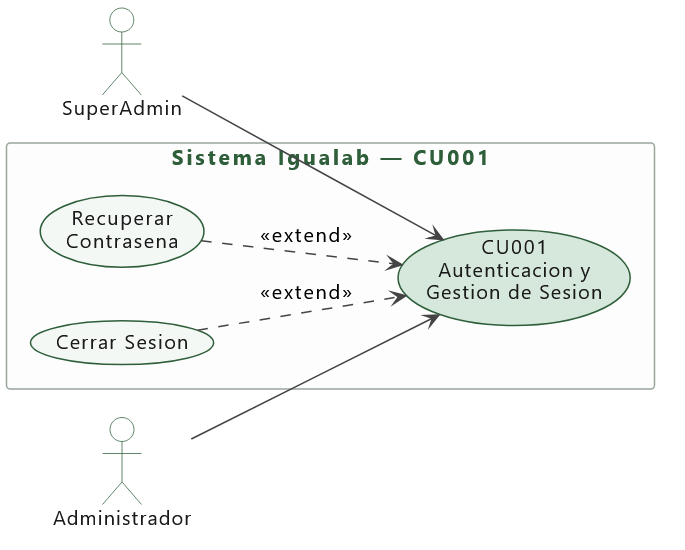
\includegraphics[width=0.78\textwidth]{img/im-019-011.png}}
\figframe{Prototipo --- CU001}{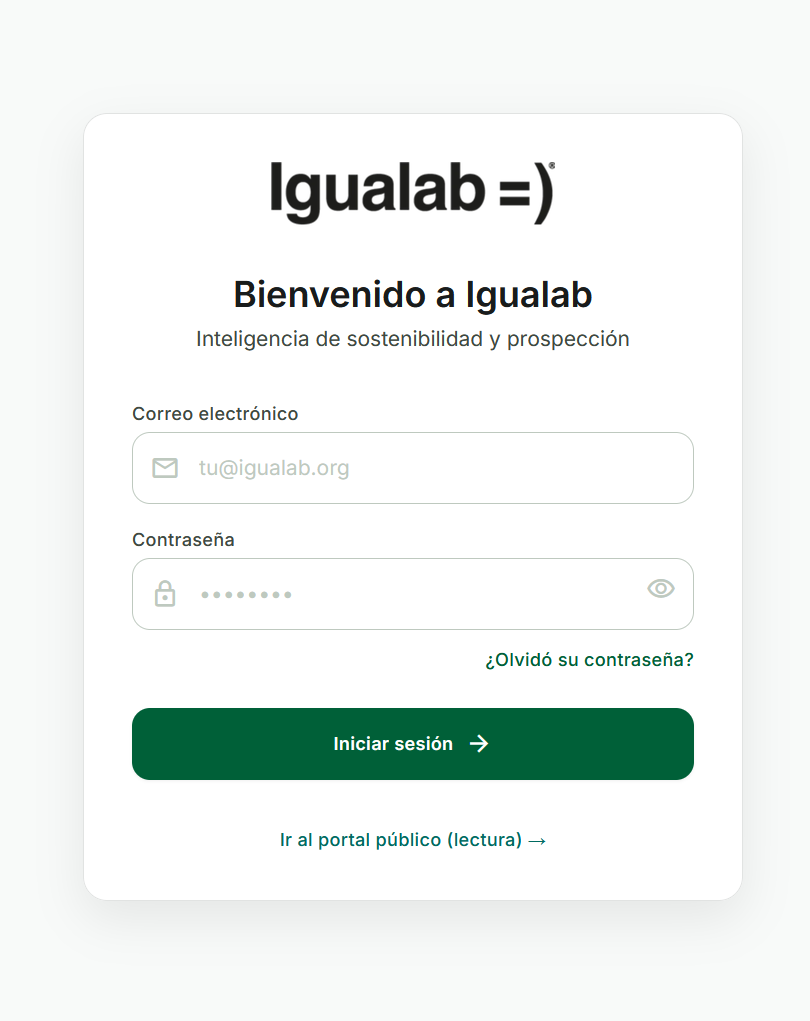
\includegraphics[width=0.52\textwidth]{img/im-020-012.png}}

% ------------------------------- CU002 -------------------------------
\clearpage
\subsubsection*{CU002: Gestión de Usuarios}
\addcontentsline{toc}{subsubsection}{CU002: Gestión de Usuarios}
\ficha{
\frow{Descripción}{Este caso de uso permite al SuperAdmin realizar la administración de las cuentas del sistema: crear cuentas (a las que se asigna automáticamente el rol Administrador), habilitar y deshabilitar cuentas de Administrador, listar las cuentas existentes con su rol y estado, y transferir el rol SuperAdmin a una cuenta de Administrador existente y habilitada. La transferencia es atómica y garantiza que en todo momento exista exactamente una cuenta SuperAdmin.}
\frow{Actores}{SuperAdmin}
\frow{Precondiciones}{-- El SuperAdmin debe haber iniciado sesión exitosamente.\newline -- Para crear una cuenta, el correo ingresado no debe estar registrado previamente.\newline -- Para transferir el rol SuperAdmin, la cuenta destino debe existir, tener rol Administrador y estar habilitada.}
\frow{Flujo Básico}{\textbf{Administración de cuentas}\newline 1. El SuperAdmin accede al módulo de gestión de usuarios.\newline 2. El sistema lista las cuentas existentes mostrando, para cada una, su nombre, correo, rol y estado (habilitada o deshabilitada).\newline 3. El SuperAdmin crea una cuenta ingresando nombre, correo y contraseña.\newline 4. El sistema valida que el correo no esté registrado, crea la cuenta y le asigna automáticamente el rol Administrador.\newline 5. El sistema confirma la creación y actualiza el listado de cuentas.}
\frow{Flujo Alternativo}{\textbf{Correo ya registrado}\newline En el paso 3, el correo ingresado ya existe en el sistema. El sistema rechaza el registro e informa que el correo ya está en uso.\par\vspace{4pt}\textbf{Habilitar / deshabilitar cuenta}\newline El SuperAdmin habilita o deshabilita una cuenta de Administrador. Al deshabilitarla, el sistema invalida de inmediato todas las sesiones activas de esa cuenta y le revoca el acceso a todas las funcionalidades.\par\vspace{4pt}\textbf{Intento de deshabilitar o eliminar al SuperAdmin}\newline El sistema impide deshabilitar o eliminar la cuenta con rol SuperAdmin desde la aplicación, indicando que primero debe transferirse el rol a otra cuenta.\par\vspace{4pt}\textbf{Transferencia del rol SuperAdmin}\newline 1. El SuperAdmin selecciona como destino una cuenta de Administrador existente y habilitada.\newline 2. El sistema muestra una alerta de confirmación antes de ejecutar el cambio.\newline 3. Al confirmar, el sistema ejecuta la transferencia de forma atómica: la cuenta destino adquiere el rol SuperAdmin y la cuenta origen pasa a rol Administrador en una sola operación. Las sesiones activas aplican el rol vigente tras la transferencia.\par\vspace{4pt}\textbf{Transferencia inválida}\newline Si la cuenta destino no existe, está deshabilitada o ya tiene rol SuperAdmin, el sistema rechaza la transferencia e informa el motivo.}
\frow{Post Condiciones}{-- Éxito: las cuentas y sus estados o roles quedan persistidos; el sistema mantiene siempre exactamente una cuenta con rol SuperAdmin.\newline -- Fallo: la operación se cancela y se notifica el error, sin alterar el estado de las cuentas.}
\frow{Restricciones}{-- Solo el rol SuperAdmin puede acceder a este módulo.\newline -- En todo momento existe exactamente una cuenta con rol SuperAdmin, con independencia de su estado o de que tenga una sesión abierta; esto se garantiza además mediante una restricción de integridad en la base de datos.\newline -- La cuenta SuperAdmin inicial se crea durante el despliegue y no puede crearse desde la aplicación.\newline -- Toda cuenta creada desde la aplicación nace con rol Administrador; el rol SuperAdmin solo se obtiene por transferencia.\newline -- La transferencia del rol se ejecuta dentro de una transacción única; un fallo parcial revierte toda la operación.}
\frow{Casos de Uso Padre}{---}
}
\figframe{Diagrama de caso de uso --- CU002}{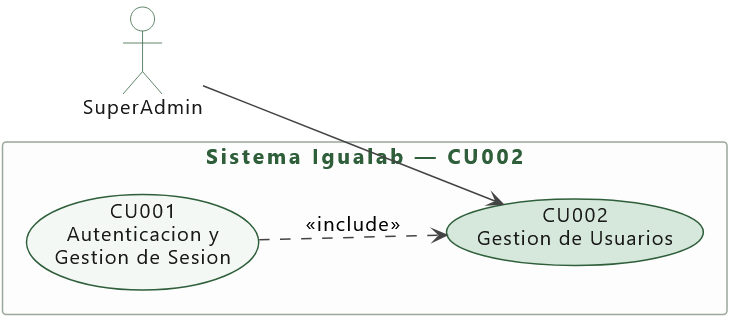
\includegraphics[width=0.72\textwidth]{img/im-022-013.png}}
\figframe{Prototipo --- CU002}{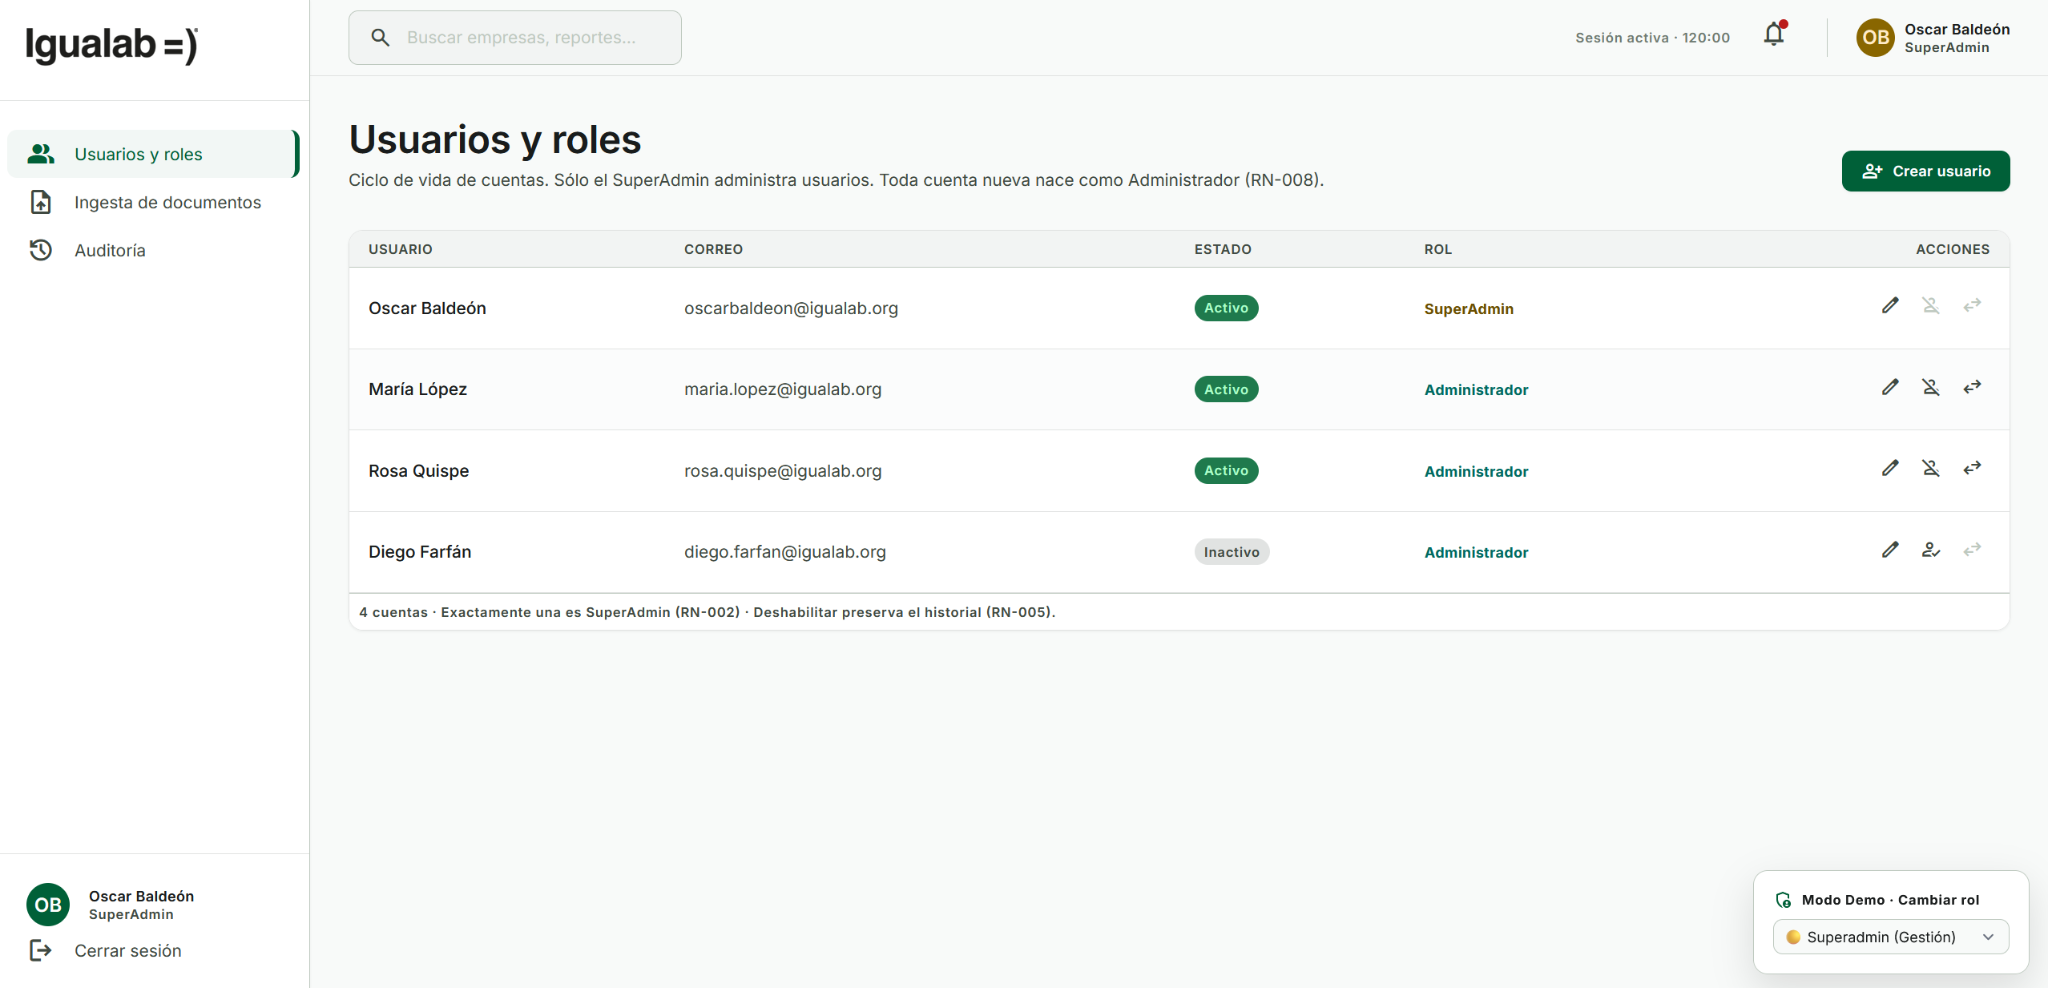
\includegraphics[width=0.9\textwidth]{img/im-022-014.png}}
\figframe{Prototipo --- CU002}{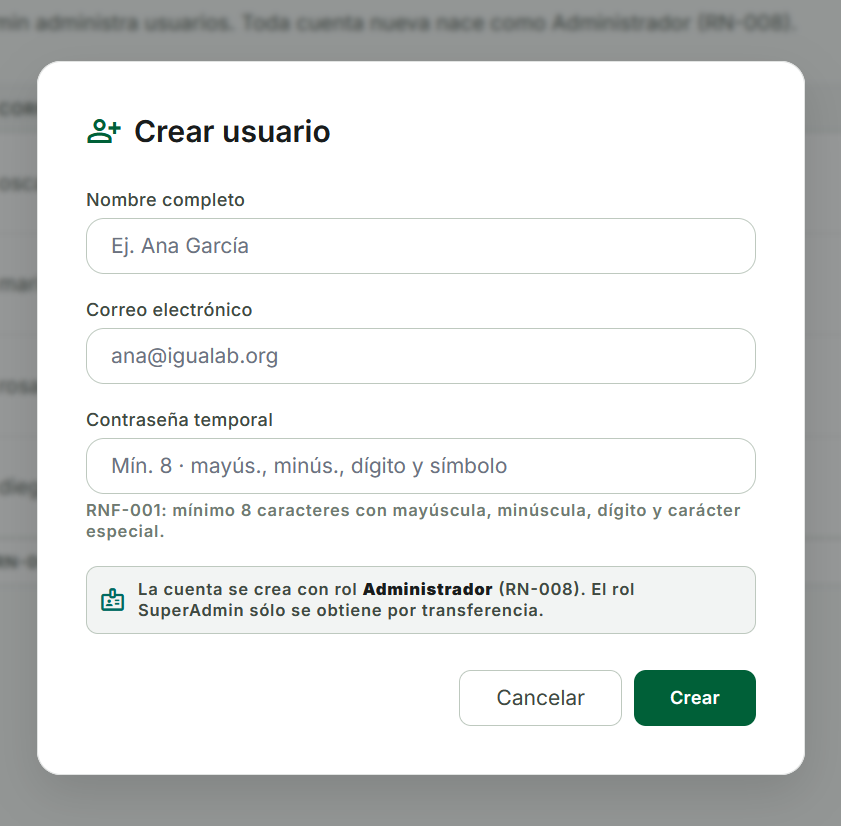
\includegraphics[width=0.62\textwidth]{img/im-023-016.png}}

% ------------------------------- CU003 -------------------------------
\clearpage
\subsubsection*{CU003: Ingesta de Documentos (memorias y reportes GRI)}
\addcontentsline{toc}{subsubsection}{CU003: Ingesta de Documentos (memorias y reportes GRI)}
\ficha{
\frow{Descripción}{Este caso de uso permite al SuperAdmin cargar memorias anuales y reportes de sostenibilidad GRI en formato Markdown (.md, con tablas de pipes), asociándolos a una empresa, un año y un tipo. El sistema valida el archivo, calcula su hash para evitar duplicados, lo indexa para el asistente y ejecuta automáticamente el análisis GRI como último paso.}
\frow{Actores}{SuperAdmin}
\frow{Precondiciones}{-- El SuperAdmin debe haber iniciado sesión exitosamente.\newline -- Debe existir la empresa (activa) a la que se asociará el documento.\newline -- El archivo debe estar en Markdown (.md), con tablas de pipes y un tamaño de hasta 50 MB.}
\frow{Flujo Básico}{\textbf{Ingesta de documentos}\newline 1. El SuperAdmin accede al módulo de Ingesta de documentos.\newline 2. Selecciona el sector y la empresa, el año y el tipo (memoria anual o reporte de sostenibilidad GRI).\newline 3. Selecciona el archivo .md y pulsa ``Ingestar''.\newline 4. El sistema valida el tipo real del archivo, el tamaño (hasta 50 MB), las tablas con pipes y el contenido mínimo (al menos un código GRI o una mención de sanción).\newline 5. El sistema calcula el hash SHA-256 y verifica la unicidad (por contenido y por empresa/año/tipo).\newline 6. El sistema procesa el documento de forma síncrona: parseo, segmentación (chunking), embeddings por API e indexación.\newline 7. Al finalizar la indexación, ejecuta el análisis GRI y de sanciones (las filas quedan sin estado, pendientes de validación humana).\newline 8. El sistema muestra el resultado (número de fragmentos indexados o el estado) y registra el evento en la auditoría.}
\frow{Flujo Alternativo}{\textbf{Empresa no registrada}\newline Si la empresa no existe, el SuperAdmin puede crearla con ``Agregar empresa'' ingresando su nombre y su sector, y reintentar la ingesta.\par\vspace{4pt}\textbf{Documento duplicado}\newline Si el contenido ya fue ingestado (mismo hash) o ya existe un documento del mismo tipo para la empresa y el año, el sistema rechaza la carga e indica la fecha y la cuenta de la carga original.\par\vspace{4pt}\textbf{Documento sin contenido analizable}\newline Si el documento no contiene ningún código GRI ni mención de sanción, el sistema lo marca como \emph{observado} (no rechazado) y no lo indexa hasta corregirse.\par\vspace{4pt}\textbf{Rechazo o interrupción}\newline Si el archivo no es .md, supera los 50 MB o el proceso se interrumpe, el sistema revierte el procesamiento (sin dejar fragmentos, embeddings ni análisis parciales) y conserva solo el motivo del rechazo.}
\frow{Post Condiciones}{-- Éxito: el documento queda indexado y el análisis GRI/sanciones poblado, listo para la revisión del Administrador.\newline -- Fallo: el documento queda como rechazado u observado con su motivo, sin incorporar contenido al corpus.}
\frow{Restricciones}{-- Solo el rol SuperAdmin puede acceder a este módulo.\newline -- Solo se admite Markdown (.md) con tablas de pipes; el sistema no convierte formatos.\newline -- Tamaño máximo por archivo: 50 MB.\newline -- La ingesta es atómica: no deja contenido parcial ante rechazo o interrupción.}
\frow{Casos de Uso Padre}{---}
}
\figframe{Diagrama de caso de uso --- CU003}{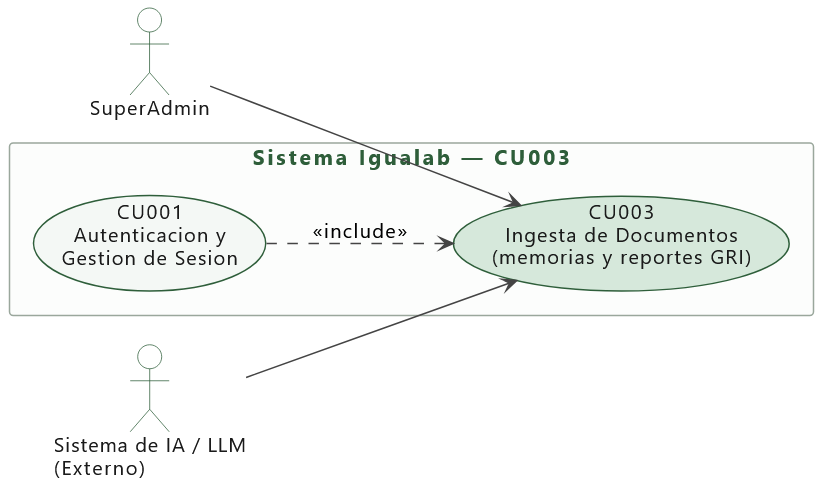
\includegraphics[width=0.72\textwidth]{img/im-025-018.png}}
\figframe{Prototipo --- CU003}{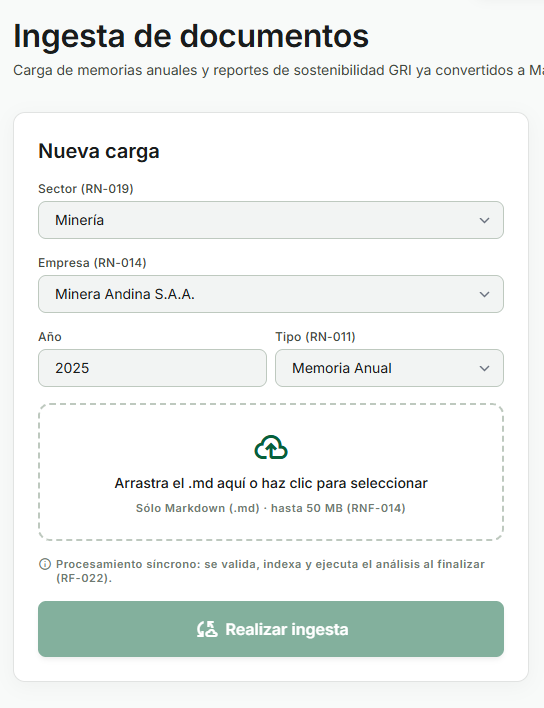
\includegraphics[width=0.62\textwidth]{img/im-026-019.png}}
\figframe{Prototipo --- CU003}{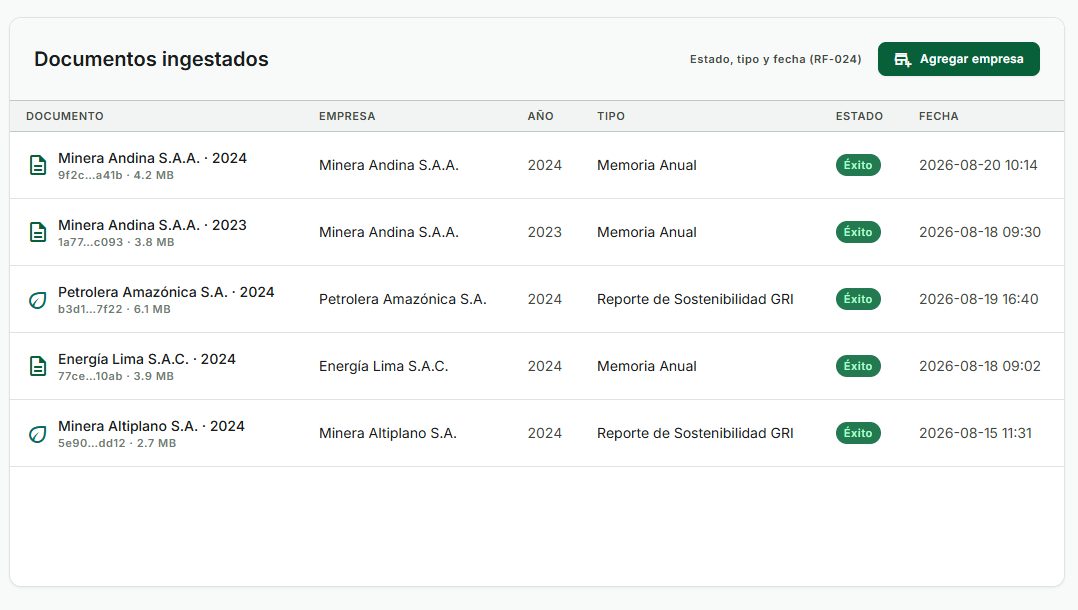
\includegraphics[width=0.92\textwidth]{img/im-026-020.png}}

% ------------------------------- CU004 -------------------------------
\clearpage
\subsubsection*{CU004: Consulta al Asistente de IA (RAG)}
\addcontentsline{toc}{subsubsection}{CU004: Consulta al Asistente de IA (RAG)}
\ficha{
\frow{Descripción}{Este caso de uso permite al Administrador usar al agente de IA para hacerle consultas dependiendo de la empresa y sector específico, también eligiendo el año de los documentos a analizar. Este puede hablar en lenguaje natural con el asistente y responderá de acuerdo a la información de los documentos en el sistema.}
\frow{Actores}{Administrador}
\frow{Precondiciones}{-- El Administrador debe haber iniciado sesión exitosamente.\newline -- Debe encontrarse en el módulo correcto para Consulta de Asistente de IA\newline -- Antes de enviar una consulta, el Administrador debe seleccionar el sector, la empresa y el año. Sin estos datos, el sistema mantiene deshabilitada la opción de consulta.}
\frow{Flujo Básico}{\textbf{Consultas al Asistente de IA}\newline 1. El Administrador accede al módulo de Consulta de Asistente de IA.\newline 2. El Administrador debe elegir el sector, empresa y año para delimitar la información que va a usar el agente de IA. El sistema muestra un mensaje inicial sobre las empresas actualmente en el sistema, y da sugerencias de prompts en lenguaje natural.\newline 3. El Administrador debe ingresar su consulta en lenguaje natural pidiendo la información pertinente de la empresa.\newline 4. El agente de IA debe procesarla, buscando información dentro de los documentos en el sistema.\newline 5. El agente de IA devuelve la respuesta conteniendo la información pedida de la consulta junto con citas para evitar información inventada.}
\frow{Flujo Alternativo}{\textbf{Información no encontrada}\newline Al devolver la información o respuesta pedida, si el documento o información pedida no existe, la IA deberá informar en su respuesta que no existe o no se encuentra, no inventarse información para cumplir con lo pedido.\par\vspace{4pt}\textbf{Consulta fuera del dominio}\newline Si la pregunta no se relaciona con sostenibilidad empresarial, indicadores GRI, sanciones o el contenido de los documentos indexados, el asistente rechaza la consulta e informa que se encuentra fuera del alcance permitido.\par\vspace{4pt}\textbf{Proveedor de IA no disponible}\newline Si el proveedor externo no responde dentro del tiempo máximo establecido, el sistema informa temporalmente la indisponibilidad del asistente. Esta situación no impide utilizar los módulos que no dependen del proveedor de IA (autenticación y gestión de usuarios, catálogo de empresas, reportes de prospección y auditoría).}
\frow{Post Condiciones}{-- Éxito: En la respuesta del agente de IA debe responder a la consulta y devolver la información solicitada.\newline -- Fallo: En su respuesta del agente de IA debe informarle al Administrador que no se encuentra la información solicitada.}
\frow{Restricciones}{-- Solo el rol Administrador tiene la capacidad de interactuar con el agente de IA.}
\frow{Casos de Uso Padre}{---}
}
\figframe{Diagrama de caso de uso --- CU004}{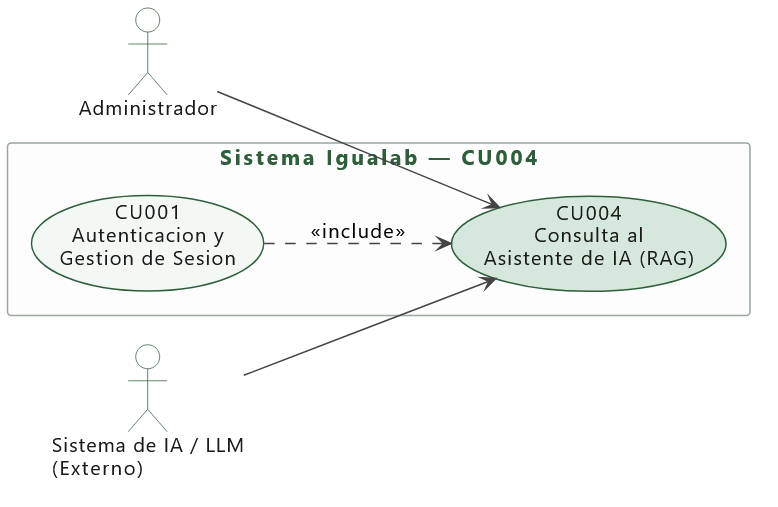
\includegraphics[width=0.72\textwidth]{img/im-028-021.png}}
\figframe{Prototipo --- CU004}{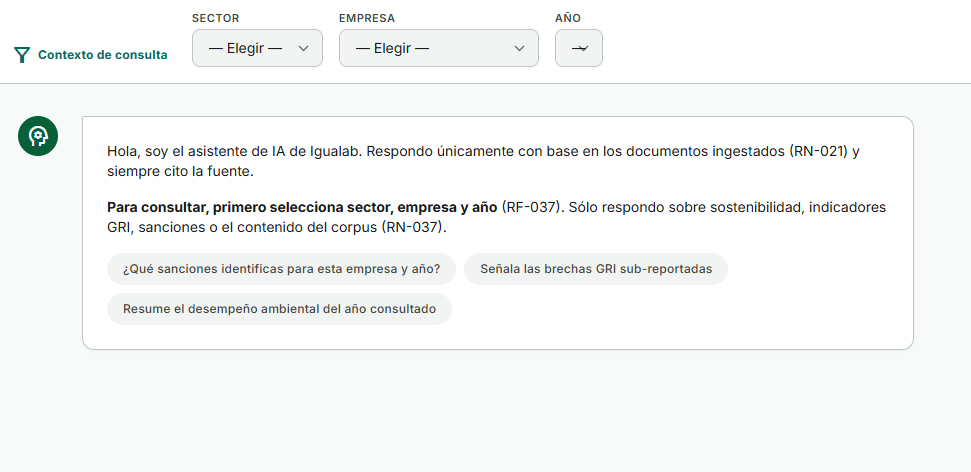
\includegraphics[width=0.85\textwidth]{img/im-028-022.png}}

% ------------------------------- CU005 -------------------------------
\clearpage
\subsubsection*{CU005: Detección de Brechas GRI y Sanciones}
\addcontentsline{toc}{subsubsection}{CU005: Detección de Brechas GRI y Sanciones}
\ficha{
\frow{Descripción}{El Administrador revisa, sobre una empresa con documentos indexados, los códigos GRI y las sanciones detectados por el sistema, y asigna \textbf{manualmente} el estado de cada código (OK, Baja sustancia o Sub-reportado). El sistema no compara el contenido contra el estándar GRI ni infiere el estado: solo detecta los códigos del catálogo presentes y extrae la cita textual de respaldo; las sanciones se toman de menciones explícitas en los documentos.}
\frow{Actores}{Administrador}
\frow{Precondiciones}{-- El Administrador ha iniciado sesión exitosamente y su sesión está vigente.\newline -- La empresa a analizar existe y tiene al menos un documento indexado.\newline -- El análisis GRI se pobló automáticamente al finalizar la ingesta.}
\frow{Flujo Básico}{\textbf{Revisión y validación de brechas}\newline 1. El Administrador accede al módulo de análisis y selecciona la empresa y el año.\newline 2. El sistema muestra los códigos GRI detectados con su \textbf{cita textual} (documento y sección) y las sanciones identificadas.\newline 3. El Administrador revisa cada cita y \textbf{asigna manualmente el estado} del código: OK, Baja sustancia o Sub-reportado.\newline 4. El sistema guarda el cambio con autor, fecha y estado anterior $\rightarrow$ nuevo (historial).\newline 5. El sistema calcula el puntaje ESG a partir de los estados asignados.\newline 6. Cuando todas las filas tienen estado, el sistema habilita la generación del reporte de prospección.}
\frow{Flujo Alternativo}{\textbf{Documentación insuficiente}\newline Si la empresa no tiene documentos indexados, el sistema informa la insuficiencia de datos y no genera resultado.\par\vspace{4pt}\textbf{Sin códigos detectados}\newline Si no se detectó ningún código GRI, el puntaje ESG se muestra como ``no disponible'' (nunca como cero) y se declara la ausencia de hallazgos.\par\vspace{4pt}\textbf{Fallo del proveedor de IA}\newline Si el servicio externo no está disponible, el sistema informa el error sin bloquear el resto de los módulos y permite reintentar.}
\frow{Post Condiciones}{-- Éxito: los estados quedan validados en la tabla del análisis, con su historial, y el resultado queda listo para generar el reporte de prospección.\newline -- Fallo: no se altera la información previamente almacenada y se notifica el motivo.}
\frow{Restricciones}{-- Solo el rol Administrador puede revisar y validar las brechas y sanciones.\newline -- El sistema no infiere ni calcula el estado; la asignación es 100\,\% manual (RN-029, RN-030).\newline -- Toda brecha y sanción reportada debe citar su fuente (documento y sección).\newline -- No se consultan fuentes externas al corpus del sistema.}
\frow{Casos de Uso Padre}{CU003 --- Ingesta de Documentos (memorias y reportes GRI)}
}
\figframe{Diagrama de caso de uso --- CU005}{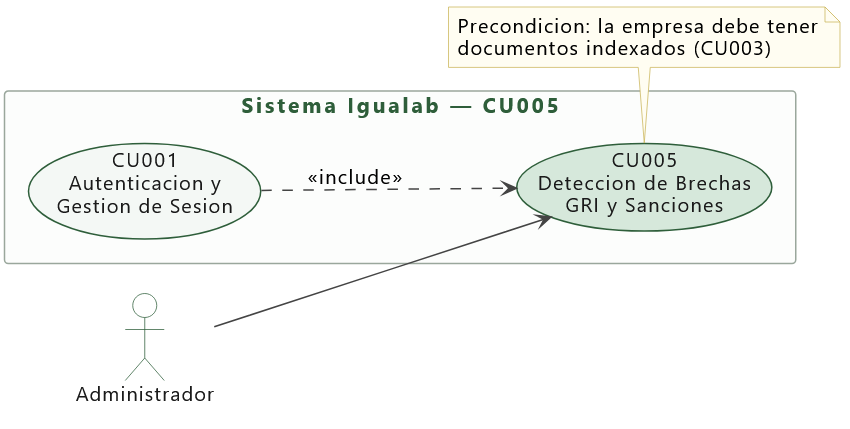
\includegraphics[width=0.72\textwidth]{img/im-030-024.png}}
\figframe{Prototipo --- CU005}{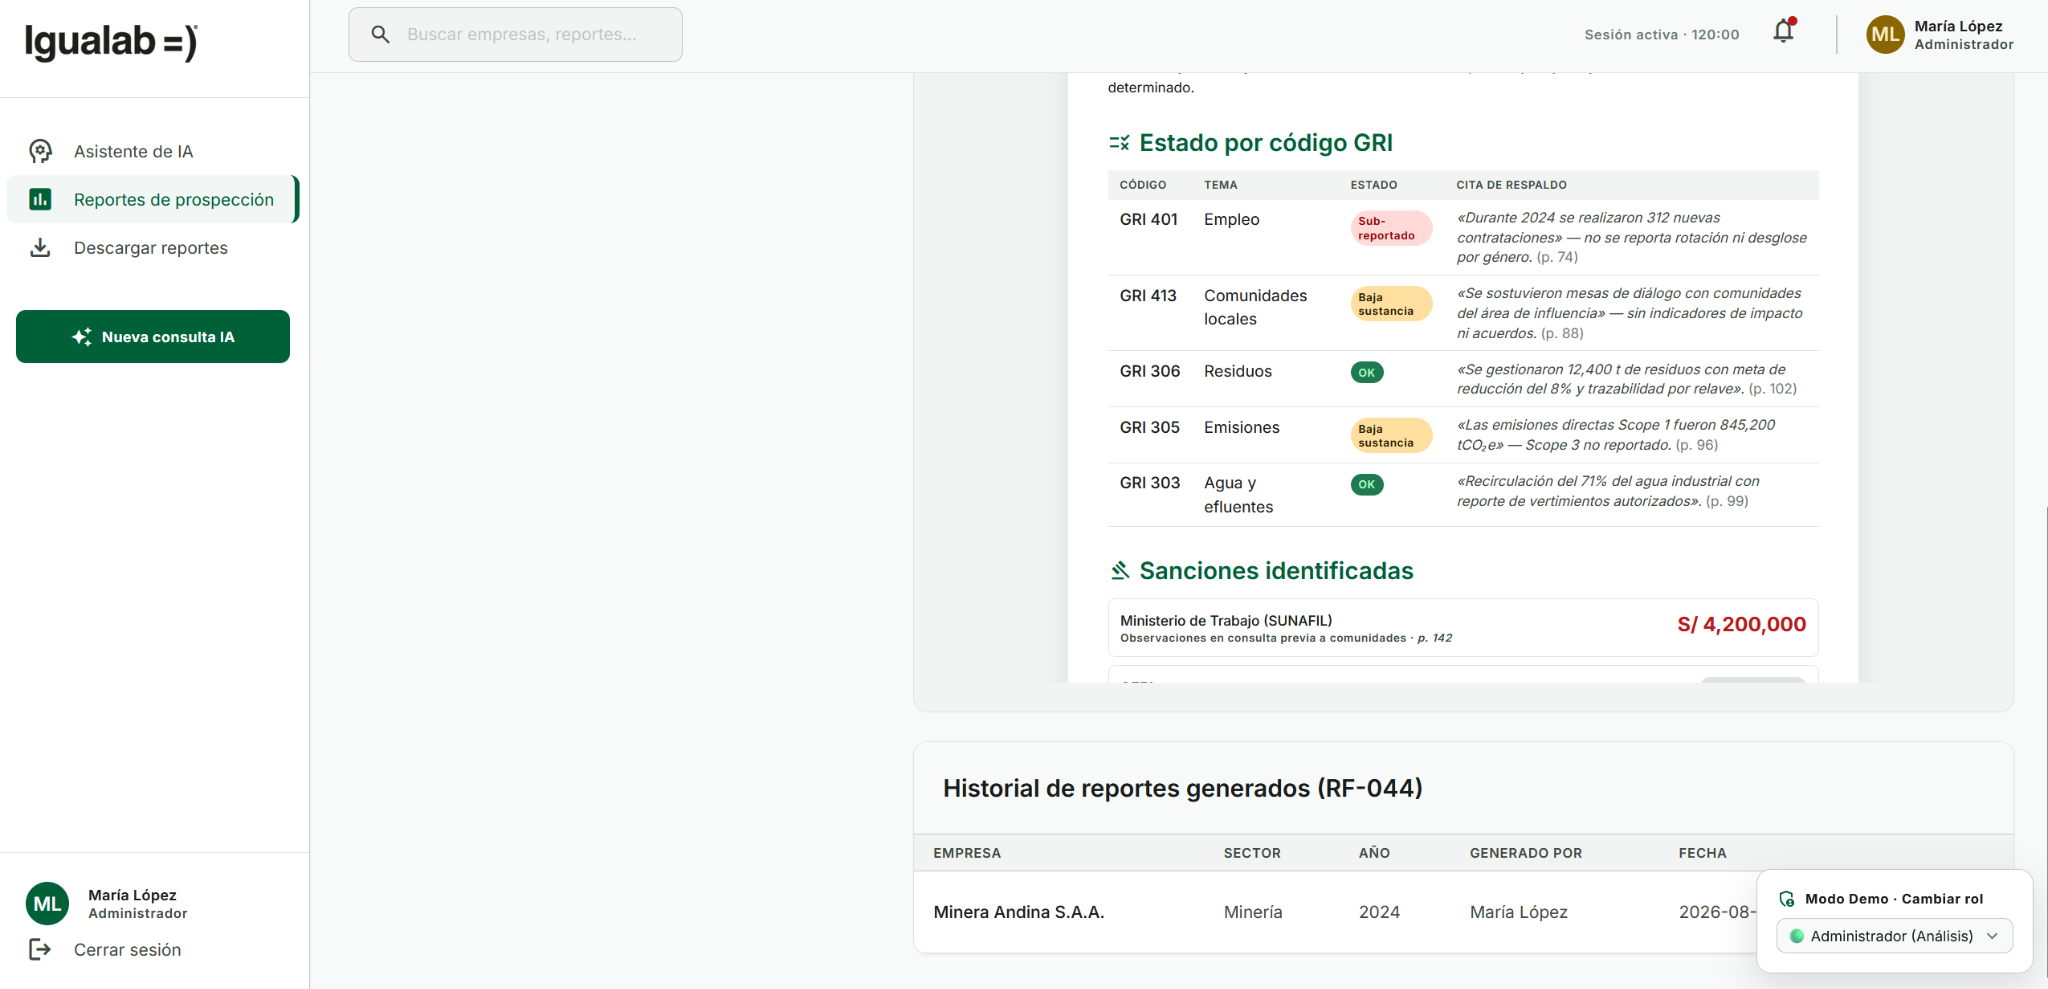
\includegraphics[width=0.9\textwidth]{img/im-031-025.png}}

% ------------------------------- CU006 -------------------------------
\clearpage
\subsubsection*{CU006: Generación de Reportes de Prospección (PDF)}
\addcontentsline{toc}{subsubsection}{CU006: Generación de Reportes de Prospección (PDF)}
\ficha{
\frow{Descripción}{Este caso de uso permite al Administrador generar un reporte de prospección para una empresa y un año determinados. El reporte se construye a partir de los resultados GRI revisados y validados, las citas de respaldo, las sanciones identificadas y el puntaje ESG. La generación no invoca al proveedor de inteligencia artificial.}
\frow{Actores}{Administrador}
\frow{Precondiciones}{-- El Administrador debe mantener una sesión vigente.\newline -- La empresa y el año seleccionados deben contar con al menos un documento indexado.\newline -- Los resultados GRI requeridos para el reporte deben haber sido revisados y validados manualmente.\newline -- No debe existir otro reporte generado para la misma empresa y año.}
\frow{Flujo Básico}{\textbf{Generar reportes de prospección}\newline 1. El Administrador accede al módulo de reportes de prospección.\newline 2. Es necesario llenar los datos del sector, empresa y año del cual se generará dicho documento.\newline 3. Tiene la capacidad de hacer una vista previa del documento previa a la generación y descarga del documento.\newline 4. Puede generar y descargar el documento de reporte de prospección.}
\frow{Flujo Alternativo}{\textbf{Generar reporte de un año que no haya documento}\newline El sistema no habilita la vista previa, generación o descarga del documento ya que no hay posibilidad de hacerlo.\par\vspace{4pt}\textbf{Reporte existente}\newline Si ya existe un reporte para la misma empresa y año, el sistema no genera uno nuevo y permite visualizar o descargar el reporte existente.}
\frow{Post Condiciones}{-- Éxito: El documento es generado, capaz de visualizarse y descargarse.\newline -- Fallo: El documento no es capaz de ser generado si el documento no existe.}
\frow{Restricciones}{-- Solo el rol Administrador puede acceder a este módulo.\newline -- El documento del cual se hará el reporte debe existir en el sistema.\newline -- Solo puede existir un reporte de prospección por combinación de empresa y año.}
\frow{Casos de Uso Padre}{CU005 --- Detección de Brechas GRI y Sanciones}
}
\figframe{Diagrama de caso de uso --- CU006}{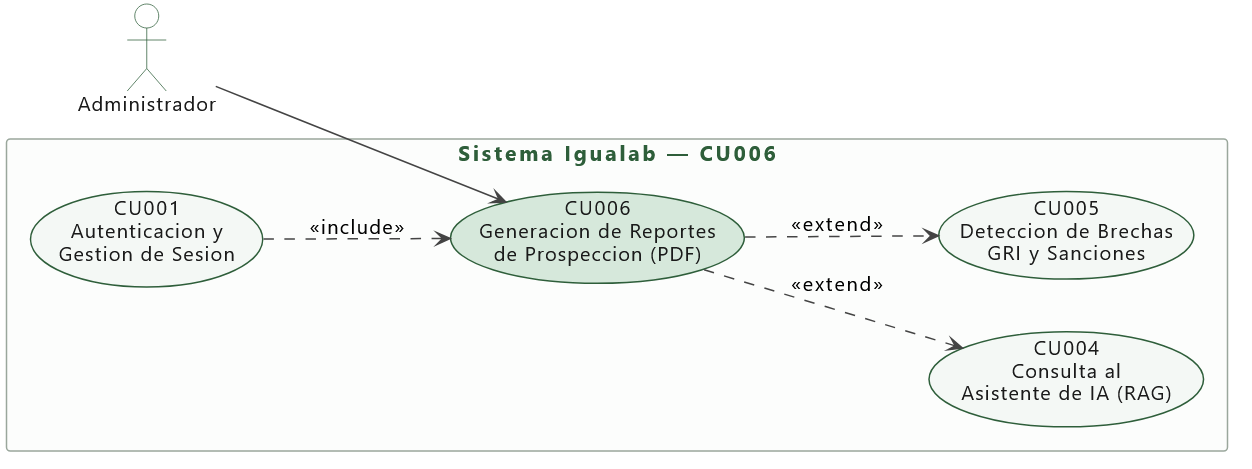
\includegraphics[width=0.85\textwidth]{img/im-032-027.png}}
\figframe{Prototipo --- CU006}{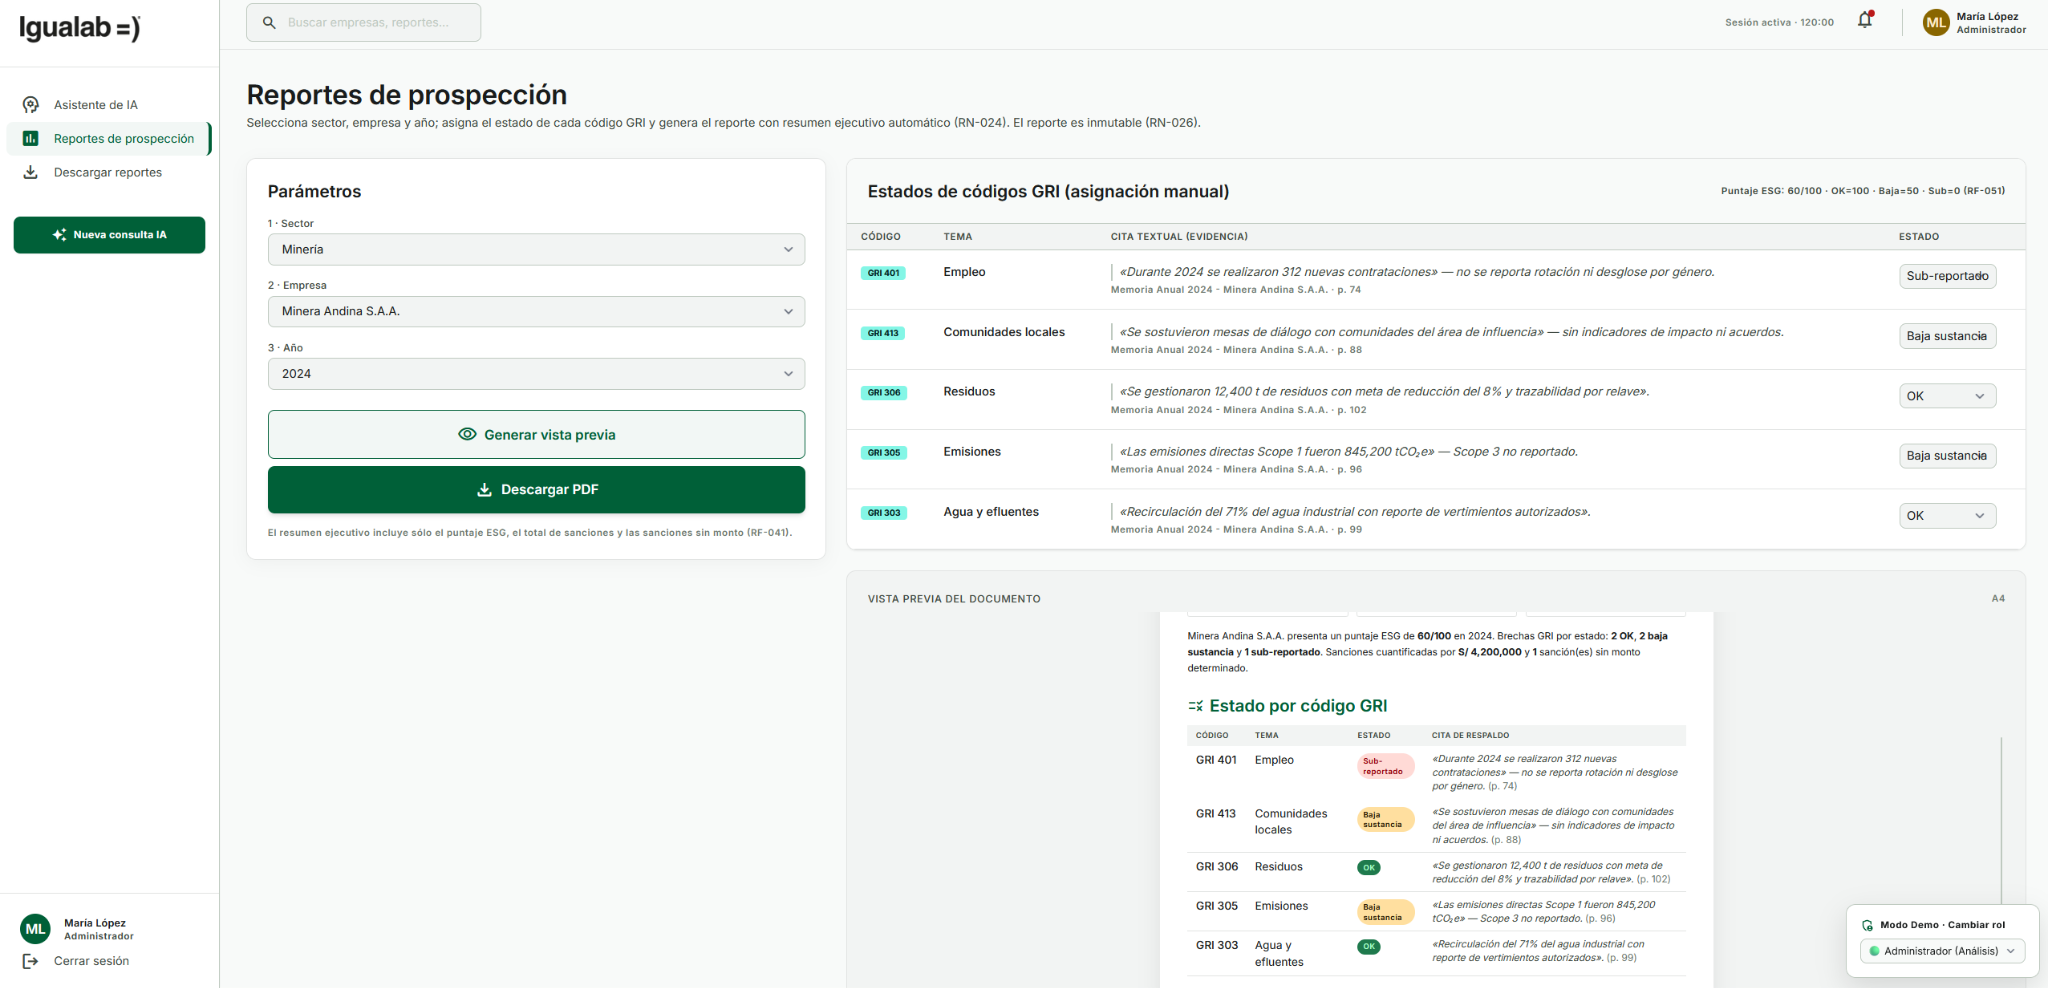
\includegraphics[width=0.9\textwidth]{img/im-032-028.png}}

% ------------------------------- CU007 -------------------------------
\clearpage
\subsubsection*{CU007: Auditoría de Eventos del Sistema}
\addcontentsline{toc}{subsubsection}{CU007: Auditoría de Eventos del Sistema}
\ficha{
\frow{Descripción}{El sistema registra automáticamente los eventos sensibles (inicios de sesión, cambios o transferencias de rol, ingesta de documentos y generación de reportes) con el usuario, la acción y la fecha, y permite al SuperAdmin consultarlos y filtrarlos para garantizar la trazabilidad y el cumplimiento de las políticas de seguridad.}
\frow{Actores}{SuperAdmin}
\frow{Precondiciones}{-- El SuperAdmin ha iniciado sesión exitosamente y su sesión está vigente\newline -- Para la consulta, existe al menos un evento registrado.}
\frow{Flujo Básico}{1. Cada vez que ocurre un evento sensible (login, cambio/transferencia de rol, ingesta, generación de reporte), el sistema lo registra automáticamente con usuario, acción, entidad afectada y fecha/hora.\newline 2. El SuperAdmin accede al módulo de auditoría.\newline 3. El sistema muestra el registro de eventos.\newline 4. El SuperAdmin aplica filtros (por usuario, tipo de evento o rango de fechas) y consulta los eventos de interés.}
\frow{Flujo Alternativo}{\textbf{Sin coincidencias}\newline En el paso 4, ningún evento cumple el filtro aplicado. El sistema informa que no hay eventos para ese criterio.\par\vspace{4pt}\textbf{Acceso no autorizado}\newline Si un rol distinto de SuperAdmin intenta acceder al módulo, el sistema deniega el acceso (HTTP 403) y registra el intento.}
\frow{Post Condiciones}{-- Los eventos sensibles quedan registrados de forma persistente y son consultables por el SuperAdmin.\newline -- La consulta no modifica los registros; el log es de solo lectura al consultarse.}
\frow{Restricciones}{-- Solo el rol SuperAdmin tiene acceso a esta sección.\newline -- La información registrada es inmutable.}
\frow{Casos de Uso Padre}{---}
}
\figframe{Diagrama de caso de uso --- CU007}{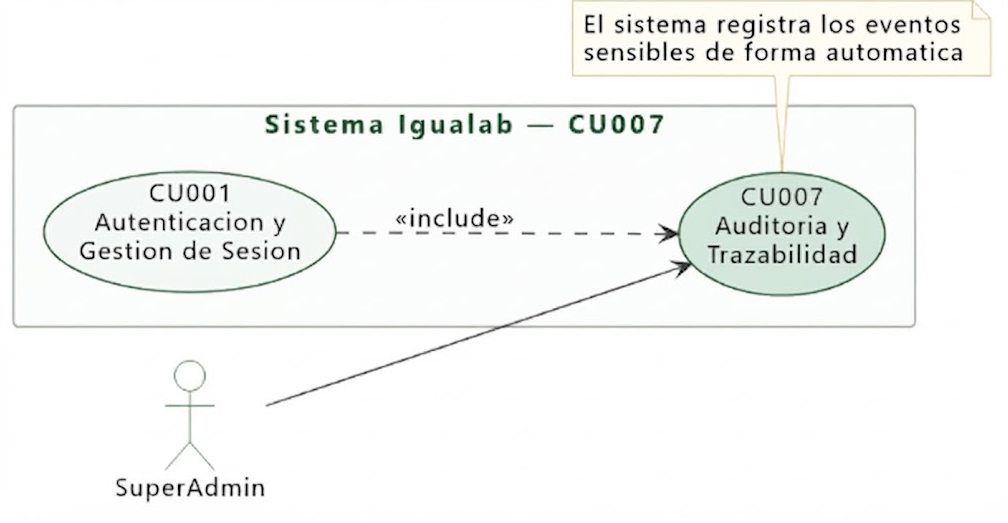
\includegraphics[width=0.72\textwidth]{img/im-033-030.png}}
\figframe{Prototipo --- CU007}{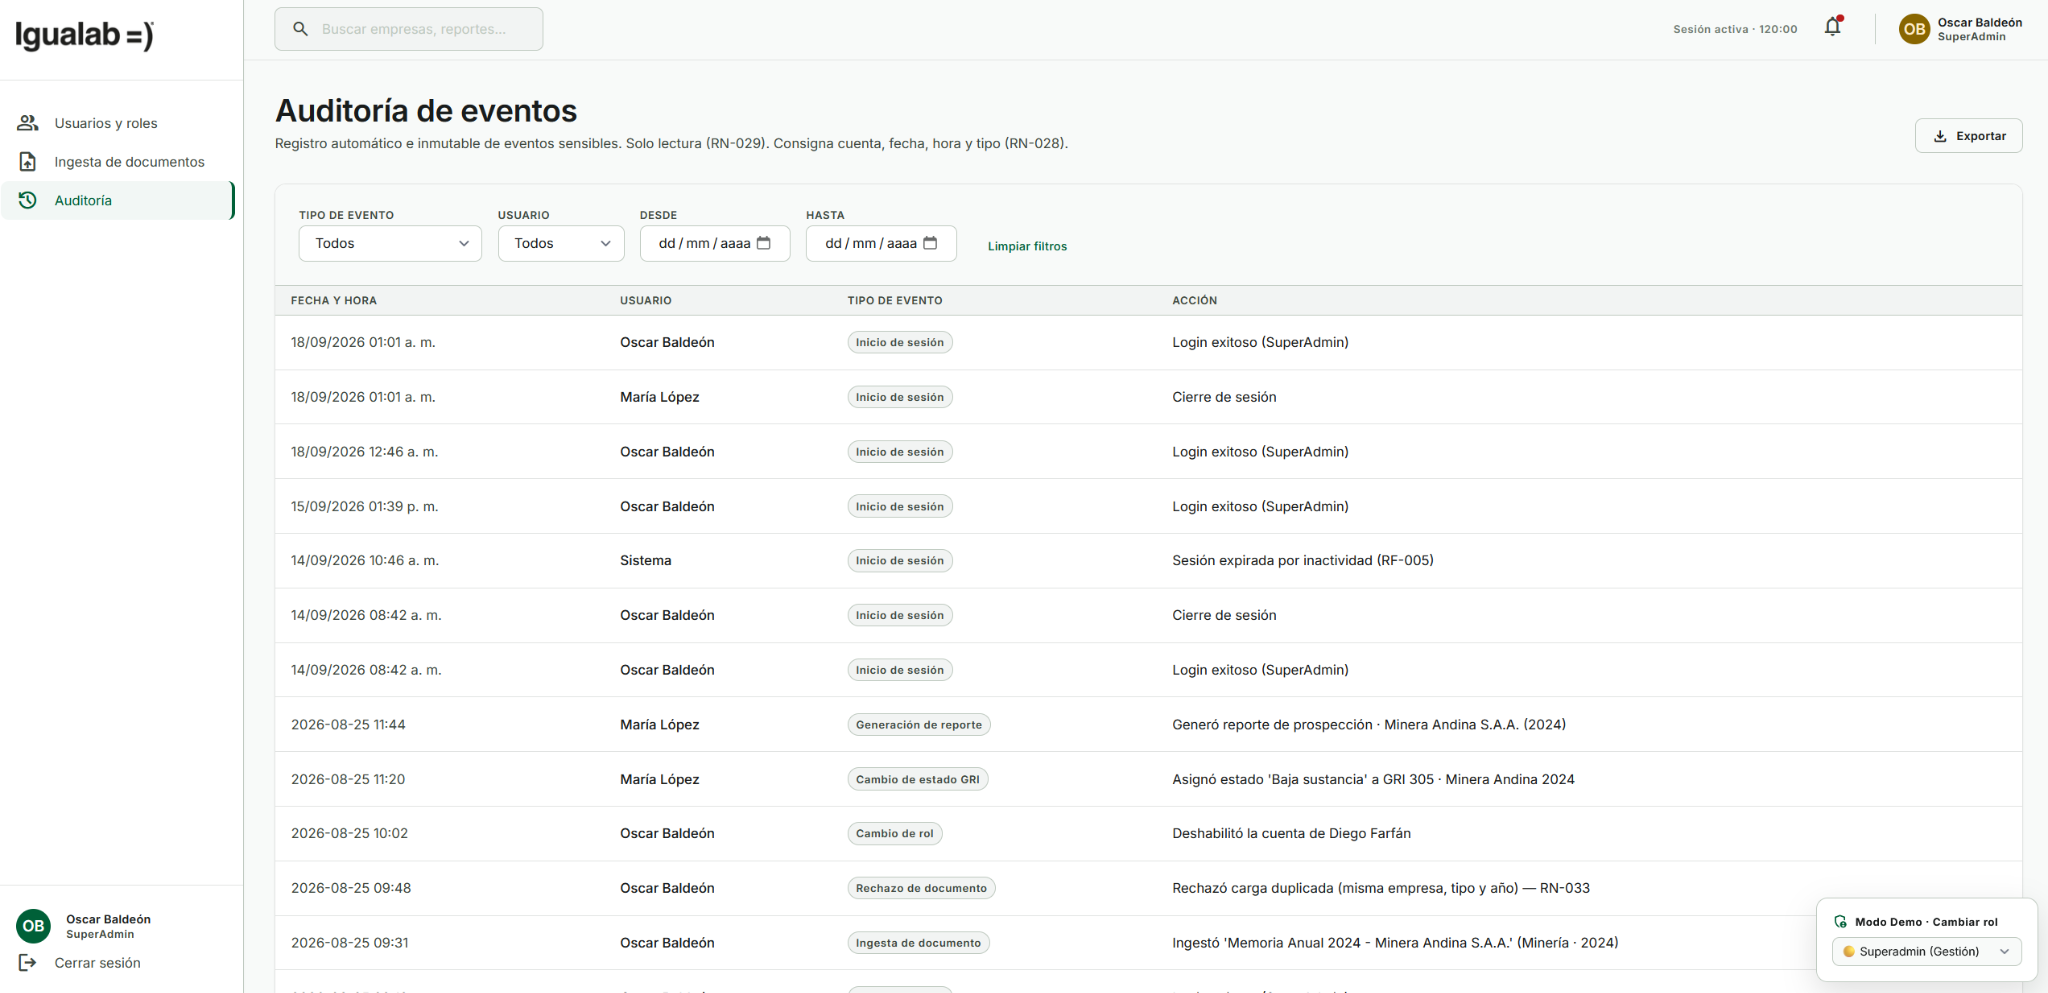
\includegraphics[width=0.9\textwidth]{img/im-034-031.png}}

% ---------------------------- 7.3 SECUENCIA --------------------------
\clearpage
\subsection{Diagrama de Secuencia}
\addcontentsline{toc}{subsubsection}{Autenticación y Gestión de Sesión}
\noindent\textbf{Caso de uso:} Autenticación y Gestión de Sesión
\begin{center}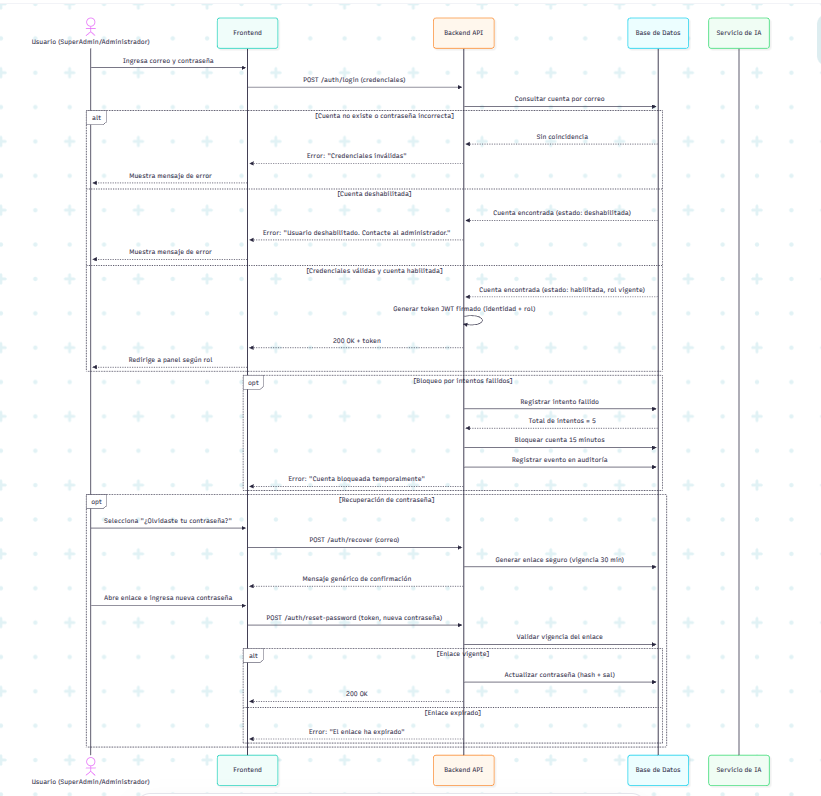
\includegraphics[width=0.85\textwidth]{img/im-034-033.png}\end{center}

\addcontentsline{toc}{subsubsection}{Gestión de Usuarios}
\noindent\textbf{Caso de uso:} Gestión de Usuarios
\begin{center}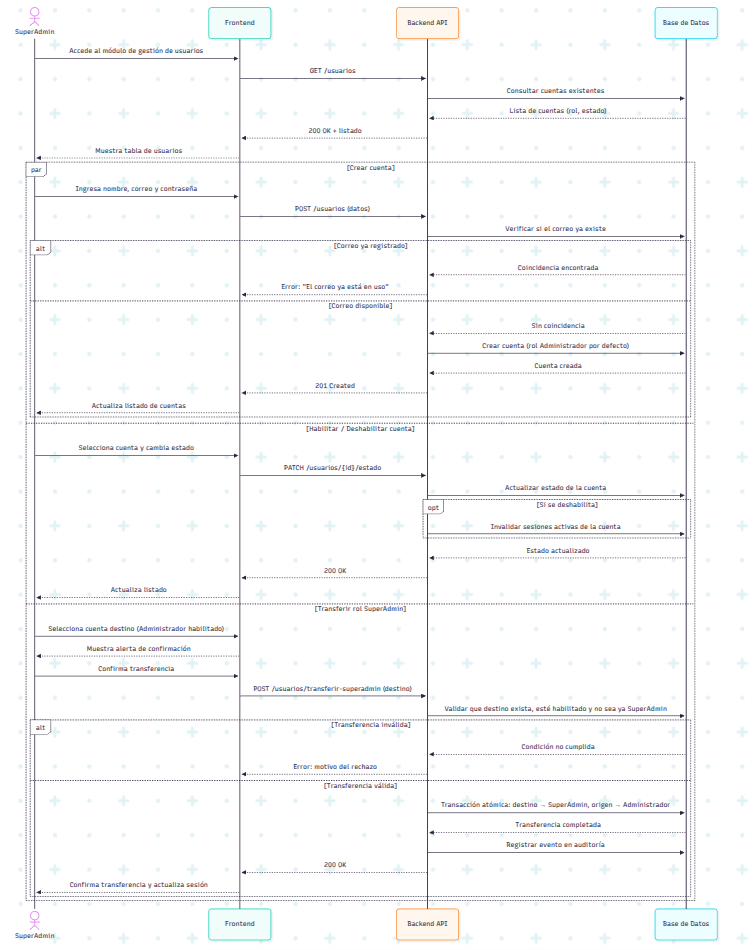
\includegraphics[width=0.85\textwidth]{img/im-035-034.png}\end{center}

\addcontentsline{toc}{subsubsection}{Ingesta de documentos (análisis GRI)}
\noindent\textbf{Caso de uso:} Ingesta de documentos (análisis GRI)
\begin{center}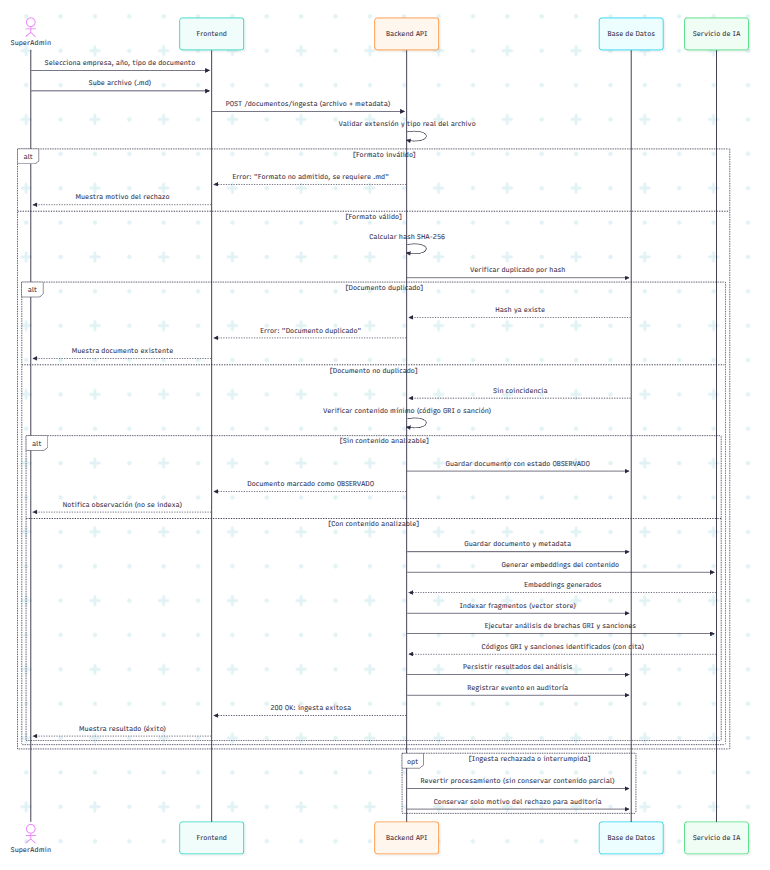
\includegraphics[width=0.85\textwidth]{img/im-036-035.png}\end{center}

\addcontentsline{toc}{subsubsection}{Consulta al Asistente de IA}
\noindent\textbf{Caso de uso:} Consulta al Asistente de IA
\begin{center}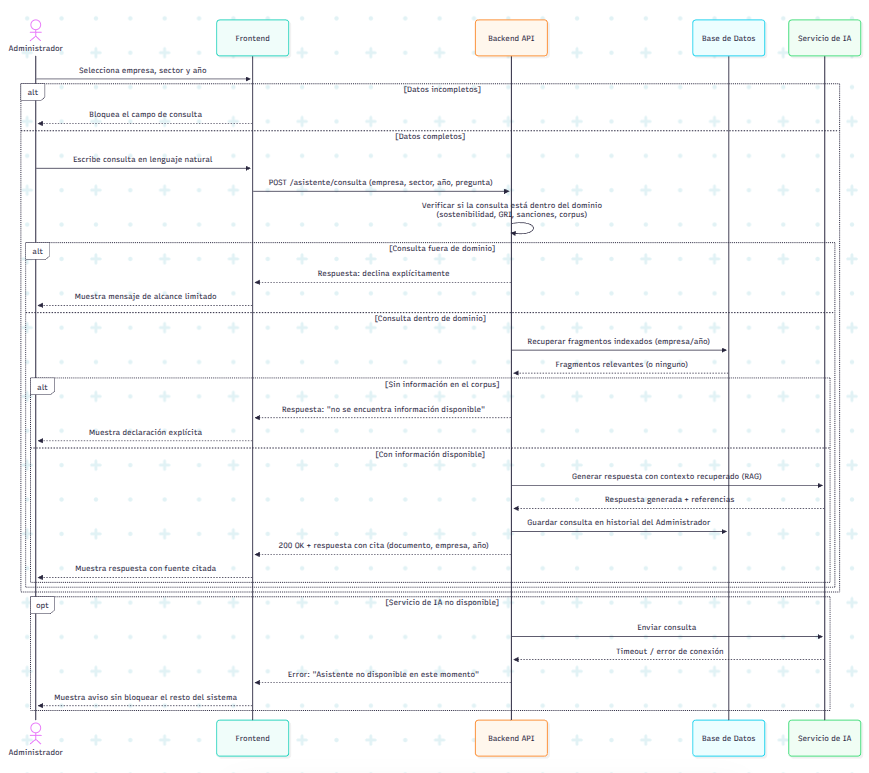
\includegraphics[width=0.85\textwidth]{img/im-037-036.png}\end{center}

\addcontentsline{toc}{subsubsection}{Detección de Brechas GRI y Sanciones}
\noindent\textbf{Caso de uso:} Detección de Brechas GRI y Sanciones
\begin{center}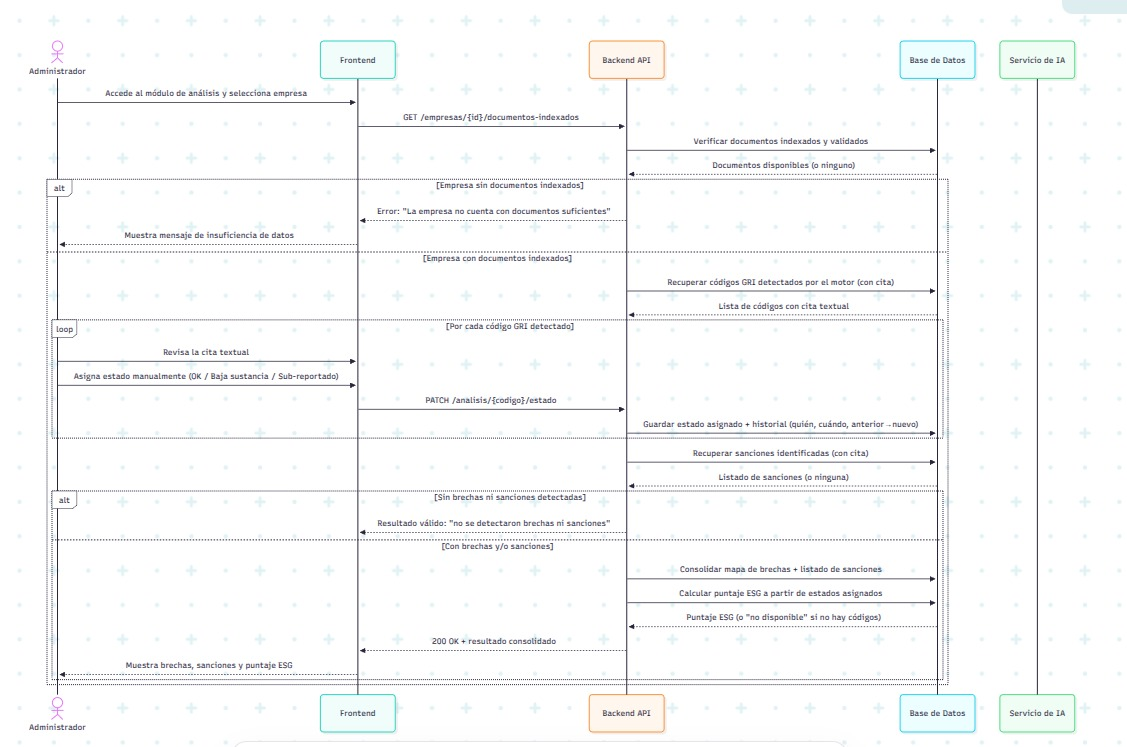
\includegraphics[width=0.85\textwidth]{img/diagrama-secuencia-CU005.jpeg}\end{center}

\addcontentsline{toc}{subsubsection}{Generación de Reportes de Prospección}
\noindent\textbf{Caso de uso:} Generación de Reportes de Prospección
\begin{center}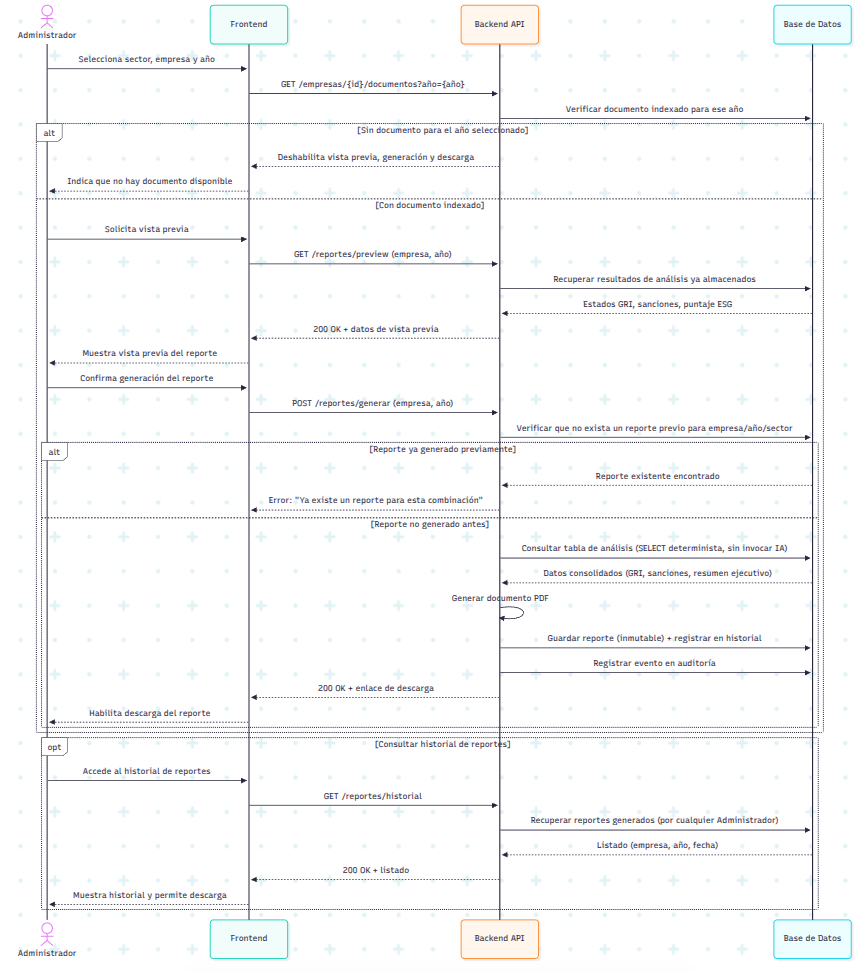
\includegraphics[width=0.85\textwidth]{img/im-038-037.png}\end{center}

\addcontentsline{toc}{subsubsection}{Auditoría de Eventos del Sistema}
\noindent\textbf{Caso de uso:} Auditoría de Eventos del Sistema
\begin{center}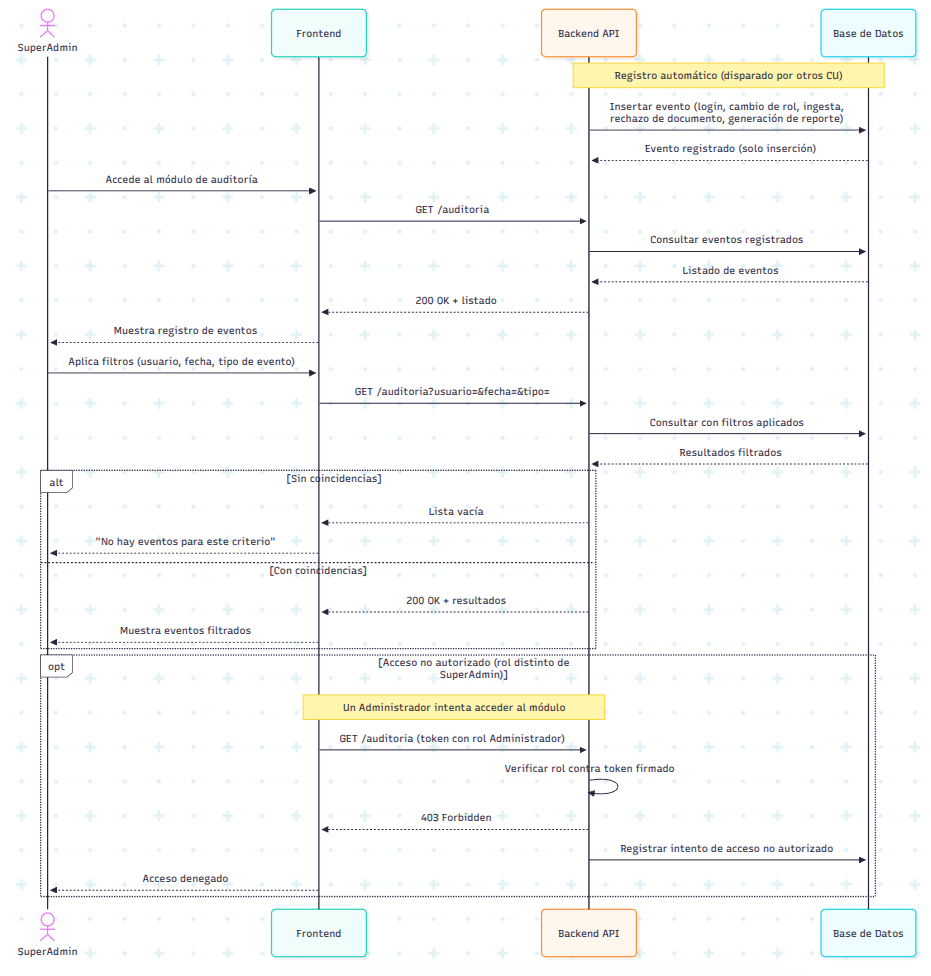
\includegraphics[width=0.85\textwidth]{img/im-039-038.png}\end{center}

% ------------------------------- 7.4 RF -------------------------------
\clearpage
\subsection{Requerimientos Funcionales}
Los requerimientos funcionales se redactan de forma atómica, verificable, comprensible y libre de implementación, y cada uno se deriva de una o varias reglas de negocio (RN). Se detallan a continuación.

La numeración de los requerimientos funcionales presentada en esta versión constituye la línea base vigente del proyecto. Cualquier artefacto anterior, caso de prueba o elemento del backlog deberá actualizar sus referencias para mantener la trazabilidad con esta versión.

\begingroup\small
% ====================================================================
%  7.4 · REQUERIMIENTOS FUNCIONALES (atómicos, derivados de RN)
% ====================================================================
\begin{longtable}{|C{1.1cm}|L{6.6cm}|L{3.1cm}|C{1.6cm}|C{1.8cm}|}
\hline
\thd{N\textdegree} & \thd{Descripción del Requerimiento Funcional} & \thd{Reglas de Negocio} & \thd{Prioridad} & \thd{Analista} \\
\hline
\endfirsthead
\hline
\thd{N\textdegree} & \thd{Descripción del Requerimiento Funcional} & \thd{Reglas de Negocio} & \thd{Prioridad} & \thd{Analista} \\
\hline
\endhead
RF-001 & Autenticar a los usuarios con correo y contraseña. & RN-004, RN-007, RN-011 & MUST HAVE & C. Ordinola \\
\hline
RF-002 & Permitir la recuperación de contraseña mediante un enlace seguro de un solo uso. & RN-010, RN-011 & MUST HAVE & C. Ordinola \\
\hline
RF-003 & Permitir al usuario cambiar su propia contraseña estando autenticado. & RN-011 & NICE TO HAVE & L. Millones \\
\hline
RF-004 & Gestionar la sesión del usuario (expiración por inactividad, cierre de sesión y rol vigente). & RN-005, RN-013 & MUST HAVE & L. Millones \\
\hline
RF-005 & Bloquear temporalmente la cuenta tras 5 intentos fallidos consecutivos. & RN-012 & MUST HAVE & C. Ordinola \\
\hline
RF-006 & Crear cuentas de Administrador con nombre, correo y contraseña. & RN-002, RN-007, RN-008 & MUST HAVE & C. Ordinola \\
\hline
RF-007 & Habilitar y deshabilitar cuentas de Administrador. & RN-002, RN-005 & MUST HAVE & L. Millones \\
\hline
RF-008 & Transferir el rol SuperAdmin a una cuenta de Administrador habilitada. & RN-002, RN-006, RN-009 & MUST HAVE & L. Millones \\
\hline
RF-009 & Listar las cuentas existentes con su rol y estado. & RN-001, RN-003 & NICE TO HAVE & C. Ordinola \\
\hline
RF-010 & Registrar empresas asociándolas a un sector. & RN-014, RN-015, RN-016 & MUST HAVE & C. Ordinola \\
\hline
RF-011 & Activar y desactivar empresas del catálogo. & RN-017 & NICE TO HAVE & L. Millones \\
\hline
RF-012 & Cargar documentos Markdown (.md) asociándolos a una empresa, un año y un tipo. & RN-018, RN-019, RN-020, RN-022 & MUST HAVE & C. Ordinola \\
\hline
RF-013 & Validar el documento cargado (formato, tamaño hasta 50 MB y contenido mínimo). & RN-021, RN-025 & MUST HAVE & C. Ordinola \\
\hline
RF-014 & Rechazar documentos duplicados por contenido o por empresa, año y tipo. & RN-023, RN-024 & MUST HAVE & L. Millones \\
\hline
RF-015 & Procesar la ingesta de forma síncrona mostrando el progreso. & RN-026 & MUST HAVE & L. Millones \\
\hline
RF-016 & Indexar el documento para el asistente (fragmentos y embeddings). & RN-018, RN-025 & MUST HAVE & C. Ordinola \\
\hline
RF-017 & Ejecutar el análisis GRI y de sanciones al finalizar la ingesta. & RN-026, RN-027, RN-028 & MUST HAVE & C. Ordinola \\
\hline
RF-018 & Detectar los códigos GRI presentes y extraer su cita textual. & RN-027, RN-028 & MUST HAVE & L. Millones \\
\hline
RF-019 & Permitir al Administrador asignar manualmente el estado de cada código GRI. & RN-029, RN-030 & MUST HAVE & L. Millones \\
\hline
RF-020 & Identificar las sanciones mencionadas en los documentos. & RN-031 & MUST HAVE & C. Ordinola \\
\hline
RF-021 & Calcular el puntaje ESG de una empresa y un año. & RN-032 & MUST HAVE & C. Ordinola \\
\hline
RF-022 & Consultar el listado de documentos ingestados con su estado. & RN-022, RN-025 & NICE TO HAVE & L. Millones \\
\hline
RF-023 & Consultar al asistente en lenguaje natural sobre el corpus indexado. & RN-033, RN-034, RN-037 & MUST HAVE & C. Ordinola \\
\hline
RF-024 & Recibir respuestas con citas y con el dominio restringido a sostenibilidad. & RN-034, RN-035, RN-036 & MUST HAVE & L. Millones \\
\hline
RF-025 & Generar el reporte de prospección en PDF a partir de los resultados validados. & RN-038, RN-039, RN-040 & MUST HAVE & C. Ordinola \\
\hline
RF-026 & Visualizar y descargar el historial de reportes de prospección. & RN-041 & NICE TO HAVE & L. Millones \\
\hline
RF-027 & Visualizar las brechas GRI de una empresa con su cita de respaldo. & RN-028, RN-034 & MUST HAVE & C. Ordinola \\
\hline
RF-028 & Consultar y filtrar los eventos de auditoría. & RN-042, RN-043, RN-044, RN-045 & NICE TO HAVE & L. Millones \\
\hline
\end{longtable}

\endgroup

% ------------------------------- 7.5 RNF ------------------------------
\subsection{Requerimientos No Funcionales}
Los requerimientos no funcionales definen las restricciones de calidad bajo las cuales opera el sistema y se derivan de las reglas de negocio (RN) y de los requerimientos funcionales (RF) a los que califican. Se presentan categorizados.

\begingroup\small
% ====================================================================
%  7.5 · REQUERIMIENTOS NO FUNCIONALES (categorizados · Deriva de RN/RF)
% ====================================================================
\begin{longtable}{|C{1.7cm}|L{2.9cm}|L{6.4cm}|L{3.4cm}|}
\hline
\thd{N\textdegree} & \thd{Categoría} & \thd{Descripción del Requerimiento No Funcional} & \thd{Deriva de} \\
\hline
\endfirsthead
\hline
\thd{N\textdegree} & \thd{Categoría} & \thd{Descripción del Requerimiento No Funcional} & \thd{Deriva de} \\
\hline
\endhead
RNF-001 & Seguridad & Las contraseñas deben tener un mínimo de 8 caracteres, con al menos una mayúscula, una minúscula, un dígito y un carácter especial, y no pueden coincidir con el correo de la cuenta. & RF-001, RN-011 \\
\hline
RNF-002 & Seguridad & Las contraseñas se almacenan mediante una función de hash de un solo sentido con sal única por usuario, nunca en texto plano. & RF-001, RN-011 \\
\hline
RNF-003 & Seguridad & La identidad de la cuenta se obtiene exclusivamente del token firmado (JWT), nunca de parámetros de la petición. & RF-001, RF-004, RN-003 \\
\hline
RNF-004 & Seguridad & La clave utilizada para firmar los tokens JWT se almacena fuera del código fuente mediante variables de entorno o secretos del ambiente. Su rotación no requiere modificar el código y se aplica mediante una actualización segura de la configuración y un reinicio controlado del servicio. & RF-001 \\
\hline
RNF-005 & Seguridad & La autorización se evalúa en cada endpoint, con independencia de lo que exponga la interfaz. & RN-003 \\
\hline
RNF-006 & Seguridad & La revocación de la sesión y la vigencia del rol se verifican en cada petición. & RF-004, RN-005, RN-013 \\
\hline
RNF-007 & Seguridad & El tipo real del archivo se valida en el servidor, sin confiar en la extensión declarada. & RF-013, RN-018 \\
\hline
RNF-008 & Seguridad & Las respuestas de recuperación y el mensaje de error de autenticación son idénticos para toda cuenta (no revelan su existencia). & RF-001, RF-002, RN-010 \\
\hline
RNF-009 & Seguridad & El token del enlace de recuperación se genera con un generador de números aleatorios criptográficamente seguro. & RF-002, RN-010 \\
\hline
RNF-010 & Seguridad & El contenido recuperado del corpus se trata como datos dentro del prompt, nunca como instrucciones (protección ante \emph{prompt injection}). & RF-024, RN-033, RN-034 \\
\hline
RNF-011 & Integridad & La unicidad documental por contenido emplea el algoritmo de hash SHA-256. & RF-014, RN-024 \\
\hline
RNF-012 & Integridad & La transferencia del rol SuperAdmin se ejecuta en una transacción única; un fallo parcial revierte toda la operación. & RF-008, RN-009 \\
\hline
RNF-013 & Integridad & La unicidad del SuperAdmin se garantiza mediante una restricción de integridad en la base de datos, además de la validación en la aplicación. & RN-002 \\
\hline
RNF-014 & Integridad & El modelo de datos distingue entre un valor no determinado y un valor igual a cero. & RN-031, RN-032 \\
\hline
RNF-015 & Integridad & El contenido de los documentos se procesa y almacena en UTF-8, preservando tildes y la letra «ñ» sin alteración. & RF-012, RF-016 \\
\hline
RNF-016 & Rendimiento & El sistema debe procesar la ingesta e indexación de un documento de hasta 50 MB dentro del tiempo máximo validado mediante pruebas de rendimiento, considerando la latencia y los límites del proveedor externo de embeddings. & RF-015 \\
\hline
RNF-017 & Rendimiento & El sistema debe registrar por separado el tiempo de procesamiento interno y el tiempo de respuesta del proveedor externo. Bajo condiciones normales, la respuesta completa del asistente no debe superar el límite definido durante las pruebas de rendimiento. & RF-023 \\
\hline
RNF-018 & Rendimiento & Las llamadas al proveedor de IA tienen un tiempo máximo de espera de 1 minuto, tras el cual la operación se reporta como indisponible. & RF-023 \\
\hline
RNF-019 & Disponibilidad & La indisponibilidad del proveedor de IA no degrada los módulos de gestión, ingesta, reportes de prospección ni auditoría. & RF-024, RN-033 \\
\hline
RNF-020 & Capacidad & El sistema admite y procesa documentos de hasta 50 MB por cada operación de ingesta. & RF-013, RN-021 \\
\hline
RNF-021 & Disponibilidad & El sistema ofrece una disponibilidad de al menos el 95\,\% en horario laboral (lun–vie, 8:00–20:00, hora de Perú). & Transversal \\
\hline
RNF-022 & Trazabilidad & Los registros de auditoría se almacenan en estructuras de solo inserción (\emph{append-only}), sin actualización ni eliminación. & RN-044 \\
\hline
RNF-023 & Trazabilidad & El registro de auditoría conserva sus entradas durante todo el periodo de operación del sistema. & RN-044 \\
\hline
RNF-024 & Trazabilidad & La fecha y hora de la auditoría se almacenan en UTC y se convierten a \emph{America/Lima} solo en la presentación. & RN-043 \\
\hline
RNF-025 & Trazabilidad & Todo fragmento indexado conserva la referencia a su documento de origen y a su ubicación dentro de él. & RF-016, RN-034 \\
\hline
RNF-026 & Mantenibilidad & El catálogo de 40 códigos GRI se carga mediante un script de inicialización versionado, garantizando el mismo catálogo en todos los ambientes. & RN-027 \\
\hline
RNF-027 & Mantenibilidad & El sistema integra al proveedor de IA mediante una interfaz estandarizada, de modo que cambiar de modelo o proveedor no obliga a rediseñar. & RF-023 \\
\hline
RNF-028 & Usabilidad & Durante la ingesta síncrona el sistema mantiene informado al usuario del progreso de la operación. & RF-015, RN-026 \\
\hline
RNF-029 & Usabilidad & Los mensajes de estado y de rechazo se presentan en español claro y accionable, indicando el motivo. & RF-013 \\
\hline
RNF-030 & Continuidad & Se realizan copias de seguridad diarias de la base de datos (incluido el índice vectorial) y de los documentos \texttt{.md} originales. & RF-016 \\
\hline
\end{longtable}

\endgroup

% ====================================================================
%  SECCIONES 8–13
% ====================================================================

\section{Modelo de Datos}

\subsection{Resumen del modelo}
\begin{center}
\begin{tabular}{|L{3.4cm}|L{11.6cm}|}
\hline
\thd{Propiedad} & \thd{Valor} \\
\hline
Motor & PostgreSQL 16 + extensión pgvector (base de datos vectorizada que sustenta el RAG) \\
\hline
Driver / acceso & AsyncPG (motor async de SQLAlchemy hacia PostgreSQL) \\
\hline
Arquitectura & Monolito modular \\
\hline
Total de tablas & 13 \\
\hline
Origen del diseño & ERD «Diagrama Entidad--Relación · IGUALAB --- Modelo de Datos Depurado» entregado por el equipo, con las correcciones aplicadas tras su revisión (puntos anotados en cada ficha) \\
\hline
Alcance retirado & Se retiraron 5 tablas del diseño v2 (configuración, catálogo de roles, medidor LLM separado) y se añadieron 4 nuevas \\
\hline
\end{tabular}
\end{center}

\subsection{El modelo por dominios (6 dominios --- refleja el ERD vigente)}
\begin{center}
\begin{tabular}{|L{3.2cm}|L{4.6cm}|L{6.7cm}|}
\hline
\thd{Dominio} & \thd{Tablas} & \thd{Propósito} \\
\hline
IDENTIDAD Y ACCESO & usuarios · sesiones · tokens\_recuperacion & Accounts of access, sesiones explícitas (JWT/sid) y recuperación de contraseña single-use. \\
\hline
EMPRESAS E INGESTA & empresas · documentos · fragmentos\_documento & Cadena de contenido fuente: catálogo de empresas, pipeline de ingesta .md y fragmentos vectorizados. \\
\hline
ANÁLISIS GRI & catalogo\_gri · gri\_analisis · sanciones & El estándar GRI (referencia) y la tabla única de resultados del análisis (códigos, citas, sanciones). \\
\hline
ASISTENTE RAG & consultas\_asistente · consulta\_citas & Persistencia de cada consulta al RAG con sus citas · fuentes (post-verificación de IDs). \\
\hline
REPORTES & reportes\_prospeccion & Entregable PDF inmutable + snapshot JSONB congelado a la fecha de emisión. \\
\hline
AUDITORÍA & auditoria & Bitácora append-only de eventos sensibles (solo INSERT; UTC). \\
\hline
\end{tabular}
\end{center}

\subsection{Entidades y relaciones (modelo conceptual)}
Cadena principal del negocio:

\noindent empresa $\rightarrow$ documento (.md) $\rightarrow$ fragmentos (vectorizados) $\rightarrow$ gri\_analisis $\rightarrow$ reportes\_prospeccion,\\
con: usuarios (quién hace qué) · auditoria (eventos sensibles) · catalogo\_gri (El estándar), consultas\_asistente + consulta\_citas (Asistente RAG).

Relaciones (todas 1:N salvo indicación):

\begin{enumerate}[leftmargin=1.6em,itemsep=2pt,topsep=2pt]
  \item Un usuario abre muchas sesiones y crea muchos tokens\_recuperacion.
  \item Una empresa tiene muchos documentos; un usuario crea los documentos (creado\_por).
  \item Un documento se vectoriza en muchos fragmentos\_documento; un documento produce muchas filas de gri\_analisis y cita muchas sanciones.
  \item Cada fila de gri\_analisis referencia un código del catalogo\_gri y proviene de un fragmento (fragmento\_id --- cita verificable).
  \item Una consulta\_asistente registra sus citas (consulta\_citas) enlazadas a fragmentos.
  \item Un reporte de prospección pertenece a una empresa (UNIQUE empresa+anio --- RN-041) y congela su snapshot a la fecha de emisión.
  \item Todo evento sensible registra auditoria (append-only; FK usuario/empresa NULL cuando aplica).
\end{enumerate}

\subsection{Diagrama Entidad--Relación (ERD vigente)}
ERD «Modelo de Datos Depurado» (13 tablas). El diagrama anterior Diagrama\_bd.png queda como archivo histórico.

\begin{center}
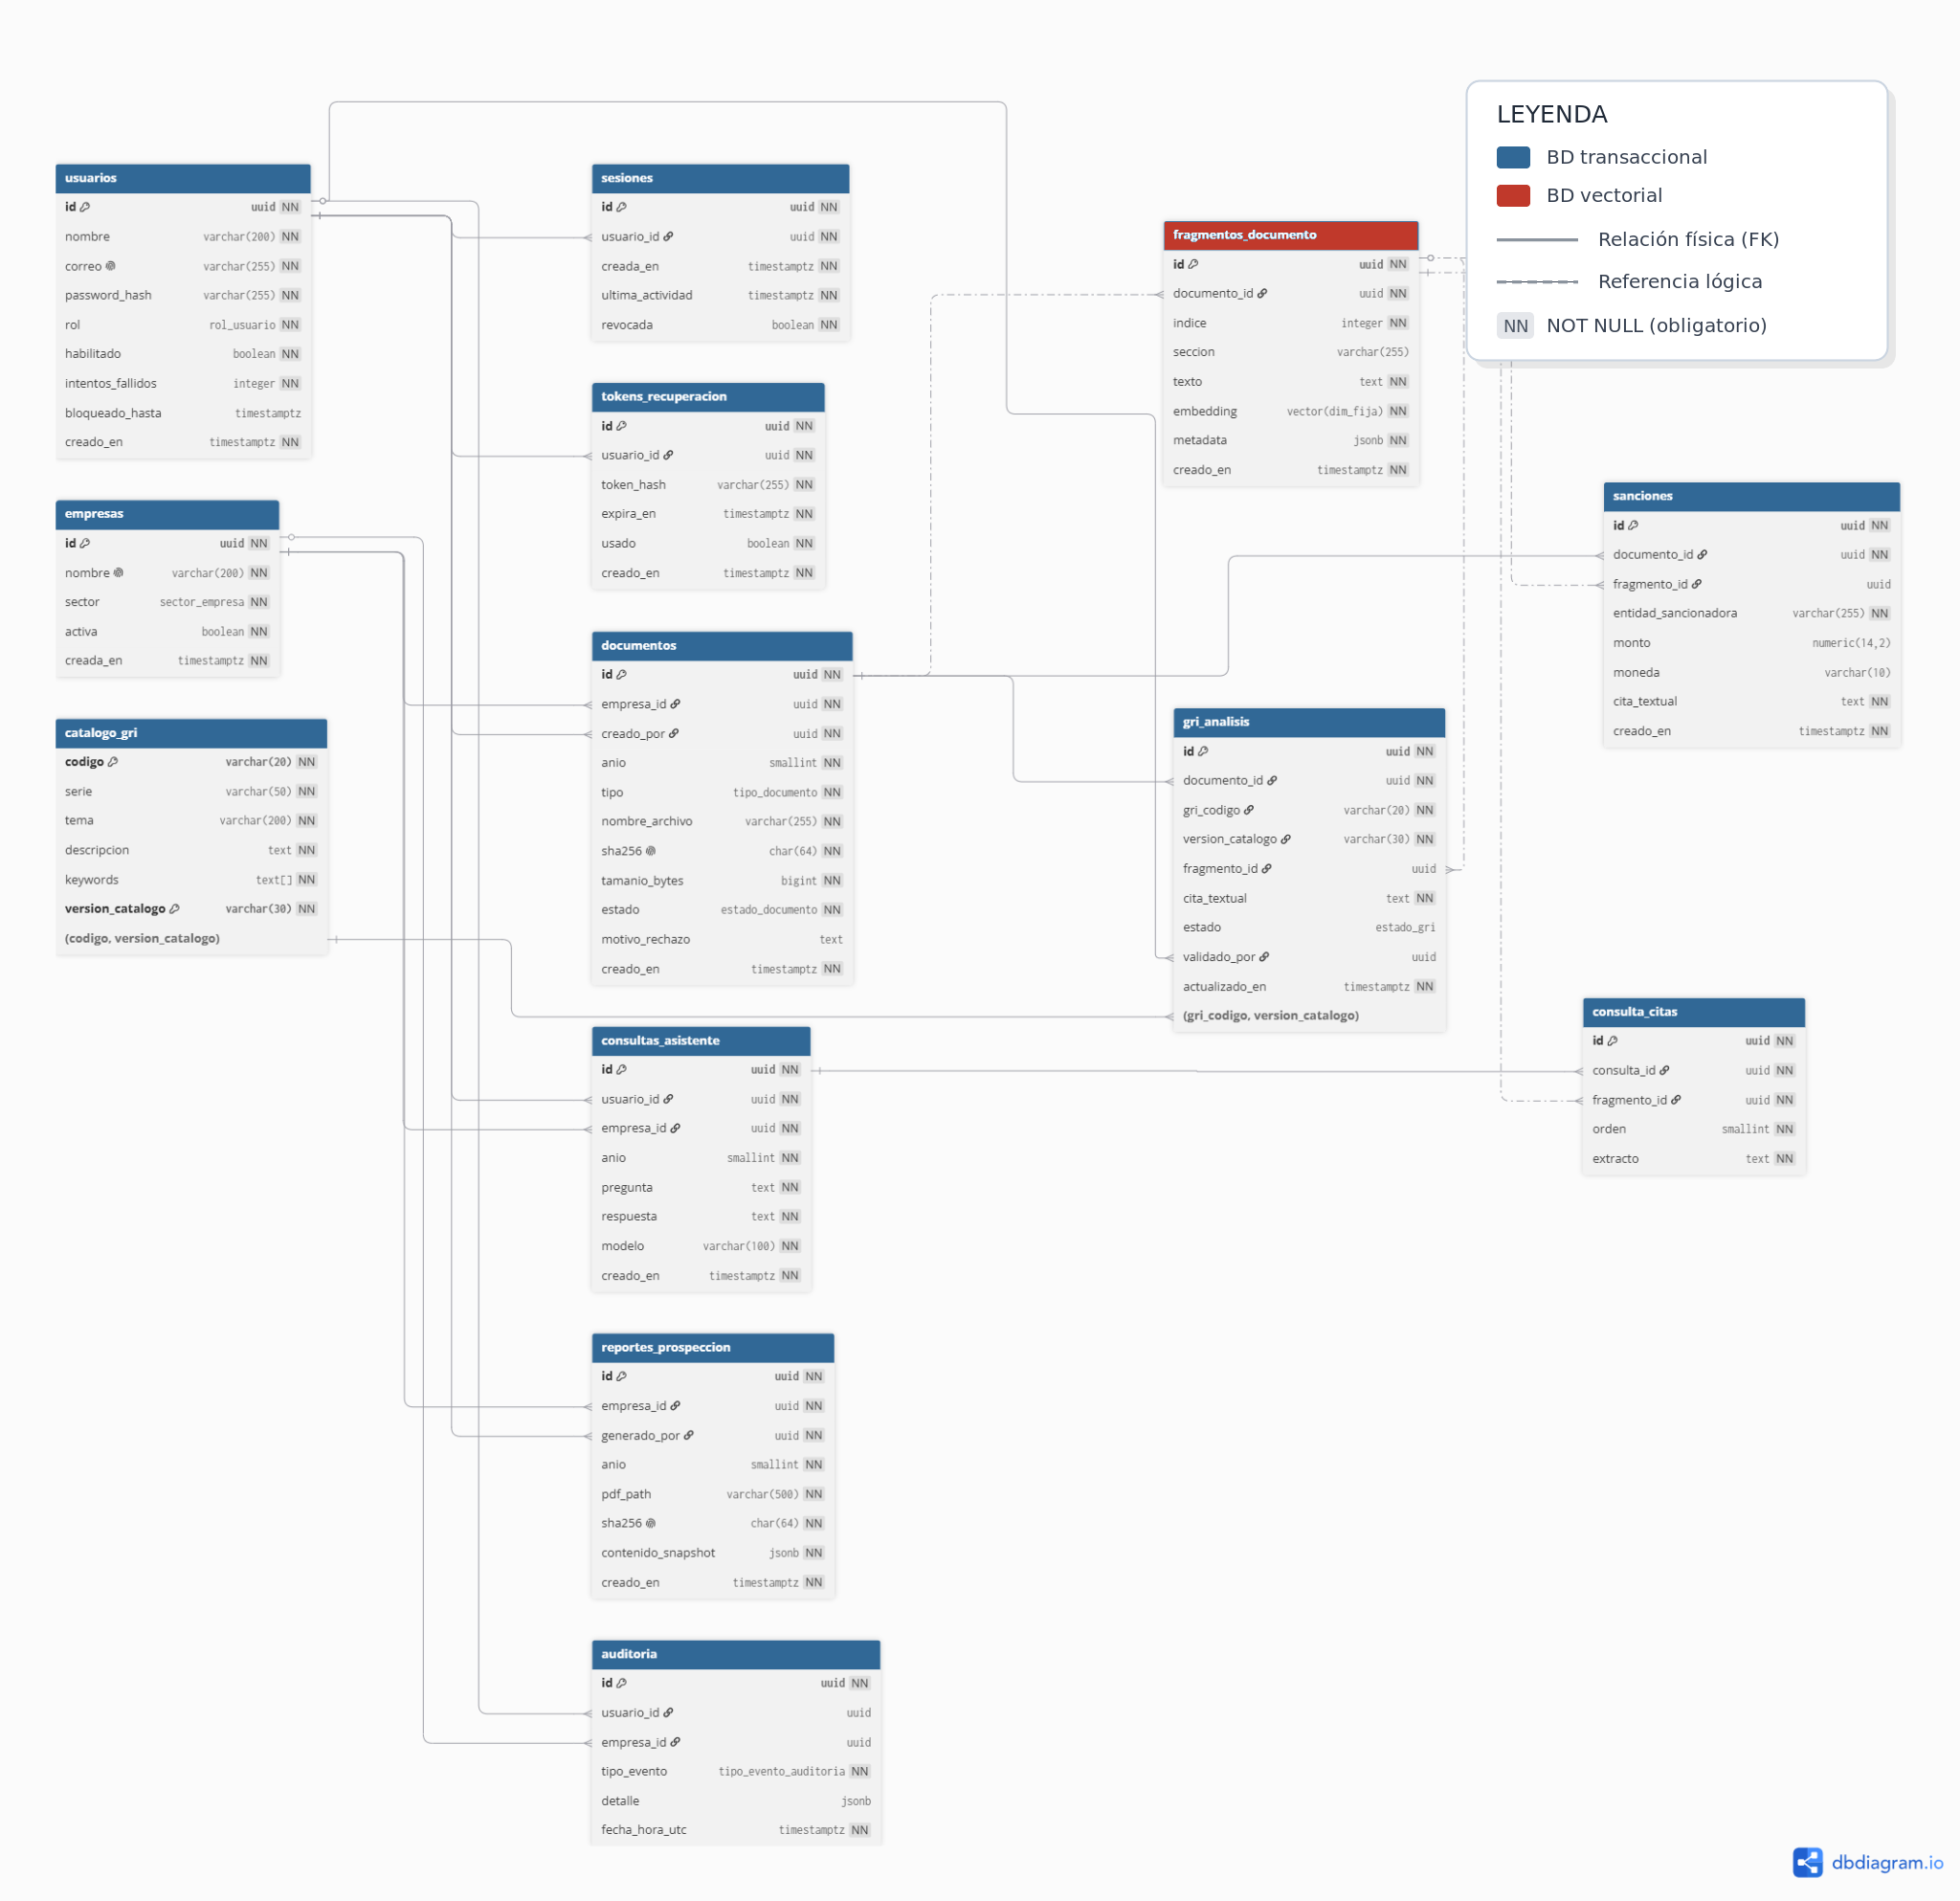
\includegraphics[width=0.95\textwidth]{img/erd-igualab.png}
\end{center}

\subsection{Restricciones clave (UNIQUE y reglas BD)}
\begingroup\small
\begin{longtable}{|L{6.9cm}|L{8.0cm}|}
\hline
\thd{Restricción} & \thd{Descripción} \\
\hline
\endhead
UNIQUE parcial en usuarios.rol (WHERE rol='superadmin') & Un solo Superadmin en toda la tabla --- la transferencia es transacción doble atómica (RS-01). \\
\hline
UNIQUE case-insensitive usuarios.correo (índice lower(correo)) & Correo único de dominio autorizado (RN-007). \\
\hline
UNIQUE documentos.sha256 & El mismo contenido nunca se ingesta dos veces (RNF-011). \\
\hline
UNIQUE parcial (empresa\_id, anio, tipo) WHERE estado='indexado' & Unicidad documental por empresa/año/tipo --- solo para documentos exitosos. \\
\hline
UNIQUE (documento\_id, indice) en fragmentos\_documento & Posición única del fragmento dentro del documento. \\
\hline
UNIQUE parcial (documento\_id, gri\_codigo) en gri\_analisis & Una sola fila de resultados por documento/código. \\
\hline
UNIQUE parcial (empresa\_id, anio) en reportes\_prospeccion & Un solo reporte por empresa/año (RN-041). \\
\hline
CHECK sectores cerrados en empresas.sector & Minería · Petróleo y Gas · Energía (RN-015, en la BD). \\
\hline
CHECK tamano\_bytes $\leq$ 50 MB en documentos & Límite de tamaño (RN-015). \\
\hline
CHECK estados ENUM & estado\_ingesta, estado\_gri, estado\_documental, tipo\_evento\_auditoria. \\
\hline
REVOKE UPDATE, DELETE en auditoria & Append-only garantizado por la BD. \\
\hline
\end{longtable}
\endgroup

\subsection{Tablas retiradas (se quitaron módulos)}
\begin{center}
\begin{tabular}{|L{4.4cm}|L{10.5cm}|}
\hline
\thd{Retirada} & \thd{Justificación} \\
\hline
roles & Catálogo cerrado de 2 filas --- sustituido por ENUM rol\_usuario + UNIQUE parcial en usuarios.rol. \\
\hline
configuracion & La tabla fue retirada; los umbrales operativos se gestionan por variables de entorno (doc Stack §4). \\
\hline
uso\_llm & El consumo diario se deriva de consultas\_asistente (COUNT por día/modelo). \\
\hline
gri\_analisis\_historico & Los cambios sensibles quedan en auditoria (AJUSTE\_BRECHA detalle JSONB). \\
\hline
reporte\_detalle\_snapshot & Sustituida por contenido\_snapshot JSONB + PDF inmutable con hash. \\
\hline
\end{tabular}
\end{center}

\subsection{Decisiones del modelo}
\begin{enumerate}[leftmargin=1.6em,itemsep=2pt,topsep=2pt]
  \item \textbf{8.7.1.} Sectores cerrados: Minería, Petróleo y Gas, Energía (CHECK en la BD).
  \item \textbf{8.7.2.} Estado GRI asignado manualmente por el Administrador: no existe estado\_sugerido.
  \item \textbf{8.7.3.} Sanciones enlazadas al documento; empresa y año se derivan de él (sin duplicar FKs).
  \item \textbf{8.7.4.} Embeddings almacenados en fragmentos\_documento; la dimensión depende del modelo del proveedor (fijar en migración, p. ej. 1024).
  \item \textbf{8.7.5.} Reporte consolidado en JSONB + PDF inmutable (sin tabla normalizada de detalle).
  \item \textbf{8.7.6.} Auditoría unipersonal separada del logging técnico y con modo append-only.
  \item \textbf{8.7.7.} FK de auditoría/consultas visibles en el diagrama (líneas largas omitidas por legibilidad).
\end{enumerate}

% ====================================================================
\section{Diccionario de Datos}

El modelo contiene 12 tablas en la base de datos transaccional y 1 tabla en la base de datos vectorial. Las relaciones entre ambas bases se registran como referencias lógicas (REF), no como claves foráneas físicas.

\newcommand{\dicthead}{\hline \thd{Campo} & \thd{Tamaño} & \thd{Tipo de Dato} & \thd{Descripción} & \thd{NULL} \\ \hline}
\newcommand{\dt}[5]{#1 & #2 & #3 & #4 & #5 \\ \hline}
\newcommand{\tabname}[1]{\par\vspace{10pt}\noindent\textbf{Tabla: #1}\par}

\par\vspace{8pt}\noindent\textbf{Base de datos transaccional:}

\tabname{usuarios}
Descripción: Almacena las cuentas de usuario, sus credenciales, rol y estado de acceso al sistema.
\begingroup\small
\begin{longtable}{|L{2.3cm}|C{1.3cm}|L{2.7cm}|L{6.4cm}|C{1.0cm}|}
\dicthead
\dt{id}{36}{UUID (PK)}{Identificador único del usuario.}{NO}
\dt{nombre}{200}{VARCHAR}{Nombre completo del usuario.}{NO}
\dt{correo}{255}{VARCHAR (UQ)}{Correo electrónico único utilizado para el inicio de sesión.}{NO}
\dt{password\_hash}{255}{VARCHAR}{Hash seguro de la contraseña del usuario.}{NO}
\dt{rol}{-}{rol\_usuario}{Rol asignado al usuario, por ejemplo SUPERADMIN o ADMIN.}{NO}
\dt{habilitado}{-}{BOOLEAN}{Indica si la cuenta está habilitada para acceder al sistema.}{NO}
\dt{intentos\_fallidos}{-}{INTEGER}{Cantidad acumulada de intentos fallidos de autenticación.}{NO}
\dt{bloqueado\_hasta}{-}{TIMESTAMPTZ}{Fecha y hora hasta la que la cuenta permanece bloqueada.}{SÍ}
\dt{creado\_en}{-}{TIMESTAMPTZ}{Fecha y hora de creación de la cuenta.}{NO}
\end{longtable}
\endgroup

\tabname{sesiones}
Descripción: Registra las sesiones iniciadas por los usuarios y permite controlar su actividad y revocación.
\begingroup\small
\begin{longtable}{|L{2.3cm}|C{1.3cm}|L{2.7cm}|L{6.4cm}|C{1.0cm}|}
\dicthead
\dt{id}{36}{UUID (PK)}{Identificador único de la sesión.}{NO}
\dt{usuario\_id}{36}{UUID (FK)}{Usuario propietario de la sesión. Referencia a usuarios.id.}{NO}
\dt{creada\_en}{-}{TIMESTAMPTZ}{Fecha y hora en que se creó la sesión.}{NO}
\dt{ultima\_actividad}{-}{TIMESTAMPTZ}{Fecha y hora de la actividad más reciente de la sesión.}{NO}
\dt{revocada}{-}{BOOLEAN}{Indica si la sesión fue invalidada antes de su expiración.}{NO}
\end{longtable}
\endgroup

\tabname{tokens\_recuperacion}
Descripción: Almacena los tokens de recuperación de contraseña y controla su vigencia y utilización.
\begingroup\small
\begin{longtable}{|L{2.3cm}|C{1.3cm}|L{2.7cm}|L{6.4cm}|C{1.0cm}|}
\dicthead
\dt{id}{36}{UUID (PK)}{Identificador único del token de recuperación.}{NO}
\dt{usuario\_id}{36}{UUID (FK)}{Usuario que solicitó la recuperación. Referencia a usuarios.id.}{NO}
\dt{token\_hash}{255}{VARCHAR (IDX)}{Hash del token enviado al usuario; se indexa para facilitar su búsqueda.}{NO}
\dt{expira\_en}{-}{TIMESTAMPTZ}{Fecha y hora de vencimiento del token.}{NO}
\dt{usado}{-}{BOOLEAN}{Indica si el token ya fue utilizado.}{NO}
\dt{creado\_en}{-}{TIMESTAMPTZ}{Fecha y hora de creación del token.}{NO}
\end{longtable}
\endgroup
Reglas semánticas: expirado o ya usado deriva a inválido. La contraseña nueva revoca todas las sesiones del usuario.

\tabname{empresas}
Descripción: Contiene las empresas evaluadas por la plataforma y la información básica de su clasificación.
\begingroup\small
\begin{longtable}{|L{2.3cm}|C{1.3cm}|L{2.7cm}|L{6.4cm}|C{1.0cm}|}
\dicthead
\dt{id}{36}{UUID (PK)}{Identificador único de la empresa.}{NO}
\dt{nombre}{200}{VARCHAR (UQ)}{Nombre único de la empresa.}{NO}
\dt{sector}{-}{sector\_empresa}{Sector económico al que pertenece la empresa.}{NO}
\dt{activa}{-}{BOOLEAN}{Indica si la empresa se encuentra activa en el sistema.}{NO}
\dt{creada\_en}{-}{TIMESTAMPTZ}{Fecha y hora de registro de la empresa.}{NO}
\end{longtable}
\endgroup

\tabname{documentos}
Descripción: Registra los documentos cargados para una empresa y controla su identificación, integridad y estado de procesamiento.
\begingroup\small
\begin{longtable}{|L{2.3cm}|C{1.3cm}|L{2.7cm}|L{6.4cm}|C{1.0cm}|}
\dicthead
\dt{id}{36}{UUID (PK)}{Identificador único del documento.}{NO}
\dt{empresa\_id}{36}{UUID (FK)}{Empresa a la que pertenece el documento. Referencia a empresas.id.}{NO}
\dt{creado\_por}{36}{UUID (FK)}{Usuario que registró el documento. Referencia a usuarios.id.}{NO}
\dt{anio}{-}{SMALLINT}{Año al que corresponde el documento.}{NO}
\dt{tipo}{-}{tipo\_documento}{Tipo de documento cargado.}{NO}
\dt{nombre\_archivo}{255}{VARCHAR}{Nombre original del archivo cargado.}{NO}
\dt{sha256}{64}{CHAR (UQ)}{Huella SHA-256 única utilizada para validar integridad y evitar duplicados.}{NO}
\dt{tamanio\_bytes}{-}{BIGINT}{Tamaño del archivo expresado en bytes.}{NO}
\dt{estado}{-}{estado\_documento}{Estado del documento dentro del flujo de ingesta y análisis.}{NO}
\dt{motivo\_rechazo}{-}{TEXT}{Motivo del rechazo cuando el documento no puede ser procesado.}{SÍ}
\dt{creado\_en}{-}{TIMESTAMPTZ}{Fecha y hora de registro del documento.}{NO}
\end{longtable}
\endgroup

\tabname{catalogo\_gri}
Descripción: Mantiene el catálogo versionado de estándares e indicadores GRI utilizados en el análisis documental.
\begingroup\small
\begin{longtable}{|L{2.3cm}|C{1.3cm}|L{2.7cm}|L{6.4cm}|C{1.0cm}|}
\dicthead
\dt{codigo}{20}{VARCHAR (PK*)}{Código del estándar GRI. Forma la clave primaria compuesta con version\_catalogo.}{NO}
\dt{serie}{50}{VARCHAR}{Serie a la que pertenece el estándar GRI.}{NO}
\dt{tema}{200}{VARCHAR}{Tema o denominación del estándar GRI.}{NO}
\dt{descripcion}{-}{TEXT}{Descripción funcional del estándar o indicador.}{NO}
\dt{keywords}{-}{TEXT ARRAY}{Palabras clave utilizadas para apoyar la identificación del estándar.}{NO}
\dt{version\_catalogo}{30}{VARCHAR (PK*)}{Versión del catálogo. Forma la clave primaria compuesta con codigo.}{NO}
\end{longtable}
\endgroup

\tabname{gri\_analisis}
Descripción: Almacena los resultados del análisis GRI identificados en cada documento y su eventual validación.
\begingroup\small
\begin{longtable}{|L{2.3cm}|C{1.3cm}|L{2.7cm}|L{6.4cm}|C{1.0cm}|}
\dicthead
\dt{id}{36}{UUID (PK)}{Identificador único del resultado de análisis GRI.}{NO}
\dt{documento\_id}{36}{UUID (FK)}{Documento analizado. Referencia a documentos.id.}{NO}
\dt{gri\_codigo}{20}{VARCHAR (FK*)}{Código GRI; integra la clave foránea compuesta hacia catalogo\_gri.}{NO}
\dt{version\_catalogo}{30}{VARCHAR (FK*)}{Versión del catálogo; integra la clave foránea compuesta hacia catalogo\_gri.}{NO}
\dt{fragmento\_id}{36}{UUID (REF)}{Referencia lógica al fragmento que sustenta el hallazgo en fragmentos\_documento.id.}{SÍ}
\dt{cita\_textual}{-}{TEXT}{Texto del documento utilizado como evidencia del hallazgo.}{NO}
\dt{estado}{-}{estado\_gri}{Estado de revisión o validación del resultado GRI.}{SÍ}
\dt{validado\_por}{36}{UUID (FK)}{Usuario que validó el resultado. Referencia a usuarios.id.}{SÍ}
\dt{actualizado\_en}{-}{TIMESTAMPTZ}{Fecha y hora de la última actualización del resultado.}{NO}
\end{longtable}
\endgroup

\tabname{sanciones}
Descripción: Registra las sanciones detectadas en los documentos y conserva la evidencia textual asociada.
\begingroup\small
\begin{longtable}{|L{2.4cm}|C{1.2cm}|L{2.6cm}|L{6.5cm}|C{1.0cm}|}
\dicthead
\dt{id}{36}{UUID (PK)}{Identificador único de la sanción.}{NO}
\dt{documento\_id}{36}{UUID (FK)}{Documento donde se identificó la sanción. Referencia a documentos.id.}{NO}
\dt{fragmento\_id}{36}{UUID (REF)}{Referencia lógica al fragmento de evidencia en fragmentos\_documento.id.}{SÍ}
\dt{entidad\_sancionadora}{255}{VARCHAR}{Nombre de la entidad que impuso la sanción.}{NO}
\dt{monto}{14,2}{NUMERIC}{Importe monetario asociado a la sanción.}{SÍ}
\dt{moneda}{10}{VARCHAR}{Código o denominación de la moneda del monto registrado.}{SÍ}
\dt{cita\_textual}{-}{TEXT}{Texto del documento que sustenta la sanción identificada.}{NO}
\dt{creado\_en}{-}{TIMESTAMPTZ}{Fecha y hora de registro de la sanción.}{NO}
\end{longtable}
\endgroup

\tabname{consultas\_asistente}
Descripción: Registra las preguntas realizadas al asistente RAG, sus respuestas y el contexto de consulta.
\begingroup\small
\begin{longtable}{|L{2.3cm}|C{1.3cm}|L{2.7cm}|L{6.4cm}|C{1.0cm}|}
\dicthead
\dt{id}{36}{UUID (PK)}{Identificador único de la consulta.}{NO}
\dt{usuario\_id}{36}{UUID (FK)}{Usuario que realizó la consulta. Referencia a usuarios.id.}{NO}
\dt{empresa\_id}{36}{UUID (FK)}{Empresa utilizada como contexto. Referencia a empresas.id.}{NO}
\dt{anio}{-}{SMALLINT}{Año utilizado como filtro de la consulta.}{NO}
\dt{pregunta}{-}{TEXT}{Pregunta formulada por el usuario.}{NO}
\dt{respuesta}{-}{TEXT}{Respuesta generada por el asistente.}{NO}
\dt{modelo}{100}{VARCHAR}{Modelo de inteligencia artificial utilizado para generar la respuesta.}{NO}
\dt{creado\_en}{-}{TIMESTAMPTZ}{Fecha y hora de ejecución de la consulta.}{NO}
\end{longtable}
\endgroup

\tabname{consulta\_citas}
Descripción: Relaciona cada respuesta del asistente con los fragmentos documentales utilizados como citas o evidencia.
\begingroup\small
\begin{longtable}{|L{2.3cm}|C{1.3cm}|L{2.7cm}|L{6.4cm}|C{1.0cm}|}
\dicthead
\dt{id}{36}{UUID (PK)}{Identificador único de la cita.}{NO}
\dt{consulta\_id}{36}{UUID (FK)}{Consulta a la que pertenece la cita. Referencia a consultas\_asistente.id.}{NO}
\dt{fragmento\_id}{36}{UUID (REF)}{Referencia lógica al fragmento citado en fragmentos\_documento.id.}{NO}
\dt{orden}{-}{SMALLINT}{Posición de la cita dentro de la respuesta.}{NO}
\dt{extracto}{-}{TEXT}{Extracto presentado como evidencia en la respuesta.}{NO}
\end{longtable}
\endgroup

\tabname{reportes\_prospeccion}
Descripción: Almacena los reportes de prospección generados para cada empresa y año, junto con su contenido consolidado.
\begingroup\small
\begin{longtable}{|L{2.3cm}|C{1.3cm}|L{2.7cm}|L{6.4cm}|C{1.0cm}|}
\dicthead
\dt{id}{36}{UUID (PK)}{Identificador único del reporte de prospección.}{NO}
\dt{empresa\_id}{36}{UUID (FK/UQ*)}{Empresa del reporte. Forma una restricción única compuesta con anio.}{NO}
\dt{generado\_por}{36}{UUID (FK)}{Usuario que generó el reporte. Referencia a usuarios.id.}{NO}
\dt{anio}{-}{SMALLINT (UQ*)}{Año del reporte. Forma una restricción única compuesta con empresa\_id.}{NO}
\dt{pdf\_path}{500}{VARCHAR}{Ruta de almacenamiento del archivo PDF generado.}{NO}
\dt{sha256}{64}{CHAR (UQ)}{Huella SHA-256 única del reporte para verificar su integridad.}{NO}
\dt{contenido\_snapshot}{-}{JSONB}{Instantánea de los datos utilizados para generar el reporte.}{NO}
\dt{creado\_en}{-}{TIMESTAMPTZ}{Fecha y hora de generación del reporte.}{NO}
\end{longtable}
\endgroup

\tabname{auditoria}
Descripción: Registra eventos relevantes del sistema para fines de trazabilidad, control y revisión.
\begingroup\small
\begin{longtable}{|L{2.3cm}|C{1.3cm}|L{2.7cm}|L{6.4cm}|C{1.0cm}|}
\dicthead
\dt{id}{36}{UUID (PK)}{Identificador único del evento de auditoría.}{NO}
\dt{usuario\_id}{36}{UUID (FK)}{Usuario relacionado con el evento. Referencia a usuarios.id.}{SÍ}
\dt{empresa\_id}{36}{UUID (FK)}{Empresa relacionada con el evento. Referencia a empresas.id.}{SÍ}
\dt{tipo\_evento}{-}{tipo\_evento\_auditoria}{Clasificación del evento registrado.}{NO}
\dt{detalle}{-}{JSONB}{Información adicional y estructurada del evento.}{SÍ}
\dt{fecha\_hora\_utc}{-}{TIMESTAMPTZ}{Fecha y hora UTC en que ocurrió el evento.}{NO}
\end{longtable}
\endgroup

\par\vspace{8pt}\noindent\textbf{Base de datos vectorial:}

\tabname{fragmentos\_documento}
Descripción: Almacena los fragmentos extraídos de los documentos, sus embeddings y metadatos para la recuperación semántica.
\begingroup\small
\begin{longtable}{|L{2.3cm}|C{1.3cm}|L{2.7cm}|L{6.4cm}|C{1.0cm}|}
\dicthead
\dt{id}{36}{UUID (PK)}{Identificador único del fragmento vectorial.}{NO}
\dt{documento\_id}{36}{UUID (REF)}{Referencia lógica al documento de origen en documentos.id, ubicado en la base transaccional.}{NO}
\dt{indice}{-}{INTEGER (UQ*)}{Posición del fragmento dentro del documento; es única en combinación con documento\_id.}{NO}
\dt{seccion}{255}{VARCHAR}{Sección o encabezado del documento al que pertenece el fragmento.}{SÍ}
\dt{texto}{-}{TEXT}{Contenido textual completo del fragmento.}{NO}
\dt{embedding}{dim\_fija}{VECTOR}{Representación vectorial del texto generada por el proveedor de embeddings.}{NO}
\dt{metadata}{-}{JSONB}{Metadatos estructurados asociados al fragmento.}{NO}
\dt{creado\_en}{-}{TIMESTAMPTZ}{Fecha y hora de creación del fragmento.}{NO}
\end{longtable}
\endgroup

% ====================================================================
\section{Volumen Estimado}
La siguiente tabla presenta una estimación del volumen mensual de datos generado por cada módulo del sistema. Los valores son referenciales y permiten identificar los módulos con mayor demanda de almacenamiento y procesamiento.

\begin{center}
\begin{tabular}{|L{4.6cm}|C{3.0cm}|C{1.5cm}|L{5.6cm}|}
\hline
\thd{Módulo} & \thd{Volumen estimado} & \thd{Nivel} & \thd{Justificación} \\
\hline
Autenticación y Gestión de Sesión & 170 registros & Medio & Considera aproximadamente 168 sesiones y 2 solicitudes de recuperación de contraseña al mes. \\
\hline
Gestión de Usuarios & 4 a 6 cuentas activas & Bajo & Referencia lógica al documento de origen en documentos.id, ubicado en la base transaccional. \\
\hline
Catálogo de Empresas & 8 a 10 empresas & Bajo & Corresponde al registro progresivo de empresas habilitadas para el análisis. \\
\hline
Ingesta de Documentos & 42 documentos y 4,200 fragmentos & Alto & Cada documento se divide en aproximadamente 100 fragmentos con embeddings para su almacenamiento en la base vectorial. \\
\hline
Análisis y Validación de Brechas GRI & 425 registros & Medio & Considera aproximadamente 417 resultados de análisis y 8 sanciones identificadas. El catálogo de 40 códigos GRI permanece como información base. \\
\hline
Asistente de Inteligencia Artificial (RAG) & 1,670 registros & Alto & Considera aproximadamente 420 consultas y 1,250 citas, con un promedio de tres citas por respuesta. \\
\hline
Generación de Reportes de Prospección & 8 a 10 reportes & Bajo & Los reportes se generan únicamente para empresas con información analizada y validada. \\
\hline
Auditoría Funcional & 420 eventos & Medio & Registra accesos, cambios de usuarios, ingestas, rechazos de documentos y generación de reportes. \\
\hline
\end{tabular}
\end{center}

% ====================================================================
\section{Diseño Arquitectónico}
La solución se estructura como una arquitectura de solución por capas, con dependencias unidireccionales de arriba hacia abajo (cada capa invoca únicamente a la inmediata inferior). Las siete capas son: actores y roles; aplicación web (SPA React 18 + Vite); API REST (FastAPI); servicios y lógica de negocio (Python 3.11, monolito modular); procesamiento y reglas por módulo; persistencia (SQLAlchemy Async); y base de datos PostgreSQL 16 con la extensión pgvector. La separación por capas y la modularidad interna (principios SOLID, con un único servicio por módulo) se detallan en la sección 4. La figura siguiente presenta el diagrama de arquitectura de solución por capas.

\begin{center}
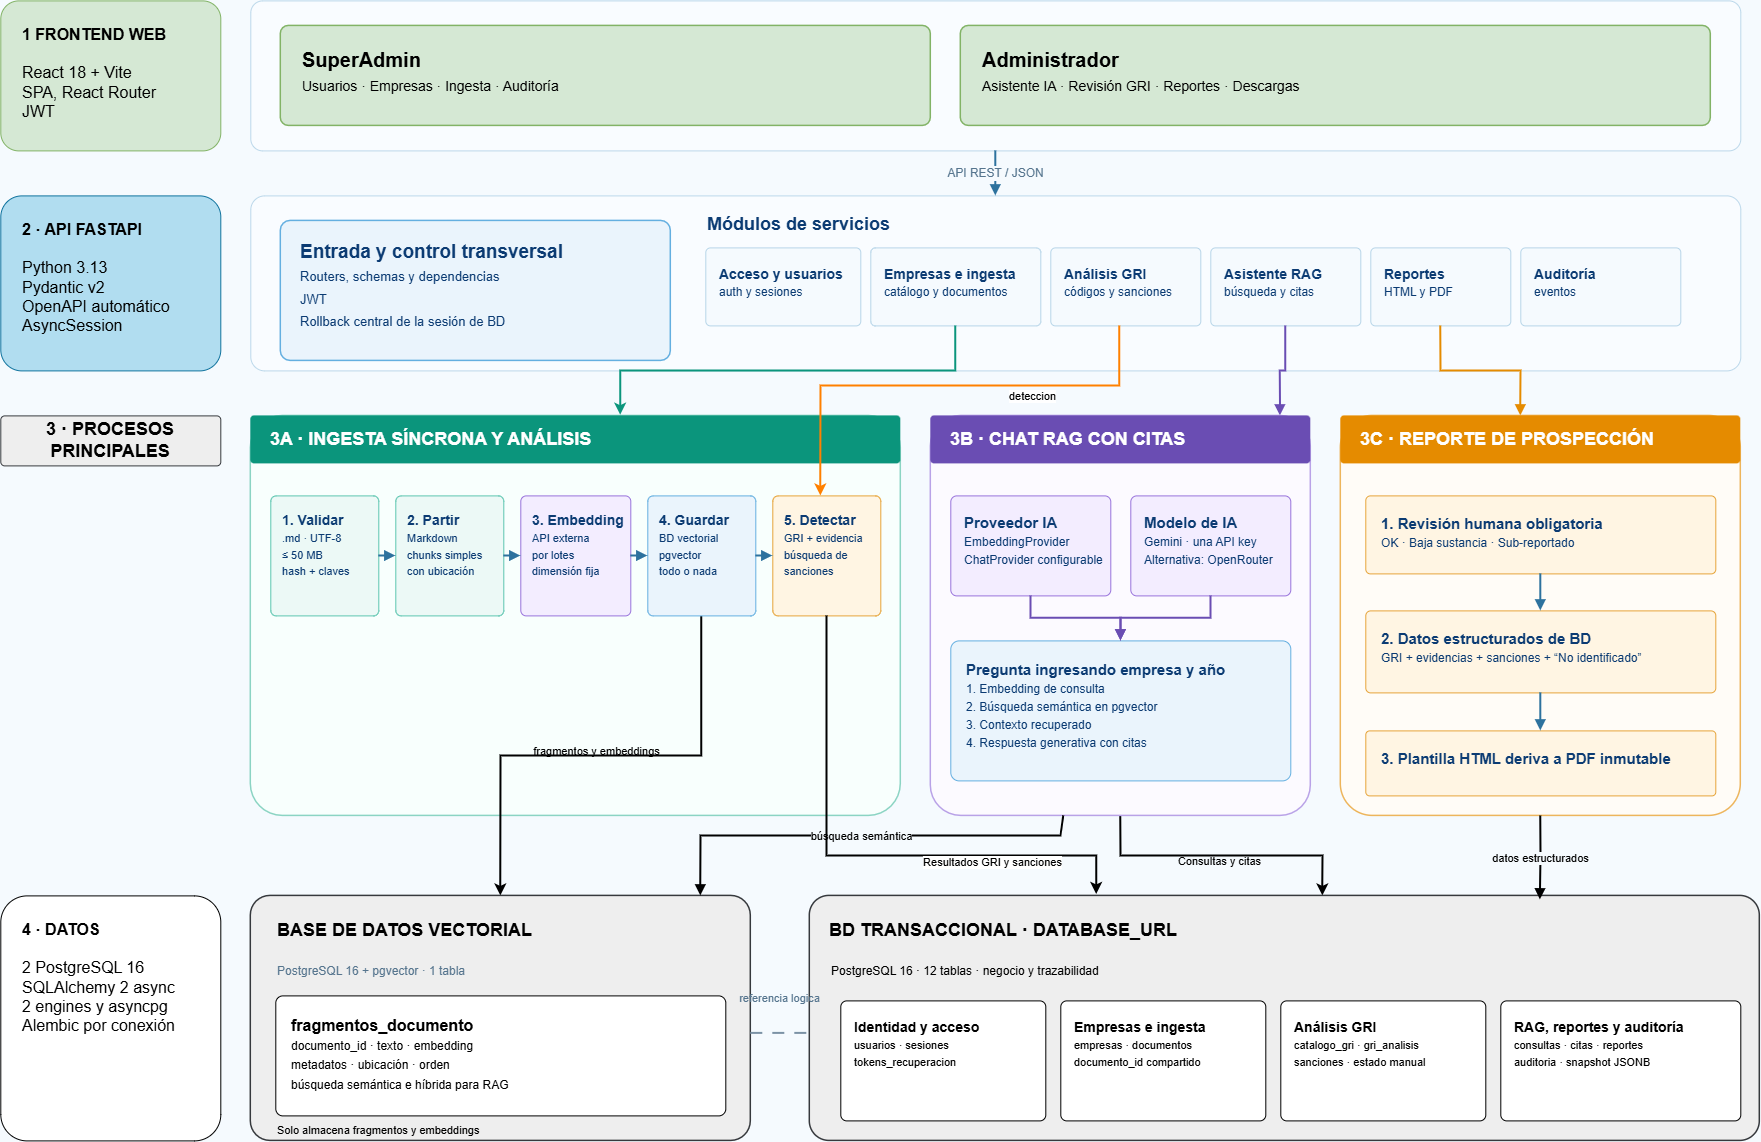
\includegraphics[width=0.98\textwidth]{img/arquitectura-igualab.png}
\end{center}

\section{Prototipo}
El prototipo navegable de la FASE 1 está disponible e implementa las pantallas de los módulos descritos en este documento (autenticación, gestión de usuarios, catálogo de empresas e ingesta, asistente de IA, reportes de prospección y auditoría), organizadas por rol: el SuperAdmin accede a la gestión de usuarios, la ingesta y la auditoría; el Administrador, al asistente de IA, los reportes y las descargas.

\section{Anexo}
\subsection{Problemas identificados del proceso actual (AS-IS)}
A partir del análisis del proceso actual (AS-IS) se identifican los siguientes problemas. El analista de Igualab debe buscar y descargar manualmente cada informe (memoria anual y/o reporte de sostenibilidad) de fuentes dispersas, lo que incrementa el riesgo de omitir documentos relevantes o descargar versiones desactualizadas. La revisión íntegra de documentos que suelen exceder las 100 páginas depende enteramente de su criterio individual, lo que genera variabilidad en la cobertura y profundidad del análisis entre distintas revisiones. No existe un catálogo estandarizado de indicadores GRI evaluables ni una metodología uniforme para asignar estados de cumplimiento, por lo que los criterios pueden variar de una empresa a otra. Una vez identificadas brechas, sanciones o hallazgos, el analista no registra la información en un sistema estructurado ni base de datos, ni hoja de cálculo, ni herramienta similar, por lo que los resultados quedan en su conocimiento implícito, sin posibilidad de consulta histórica, comparación entre empresas o trazabilidad. Tampoco se registra qué empresa revisó, en qué fecha ni con qué criterios, lo que impide validar la calidad del análisis o demostrar diligencia ante el cliente. La elaboración del documento de prospección se realiza en texto libre sin plantilla estandarizada, lo que genera formatos inconsistentes y omisión de información relevante. En conjunto, cada análisis parte de cero y no permite reutilizar resultados previos, comparar evolución año a año ni escalar el proceso a más empresas sin incrementar linealmente la carga de trabajo.

\subsection{Matriz de trazabilidad (módulo · CU · RF · RN · RNF)}
La matriz siguiente consolida la cobertura de cada módulo funcional: su caso de uso, los requerimientos funcionales que implementa y su respaldo en reglas de negocio y requerimientos no funcionales.

\begin{center}
\begingroup\small
\begin{longtable}{|C{0.7cm}|L{3.8cm}|C{1.3cm}|L{4.6cm}|L{4.3cm}|}
\hline
\thd{\#} & \thd{Módulo} & \thd{CU} & \thd{Requerimientos Funcionales (RF)} & \thd{Respaldo (RN · RNF)} \\
\hline
\endhead
1 & Autenticación y Gestión de Sesión & CU001 & RF-001…RF-005 & RN-004…RN-013 · RNF-001…RNF-009 \\
\hline
2 & Gestión de Usuarios & CU002 & RF-006…RF-009 & RN-001…RN-009 · RNF-012, RNF-013 \\
\hline
3 & Catálogo de Empresas & CU003 & RF-010, RF-011 & RN-014…RN-017 \\
\hline
4 & Ingesta de Documentos & CU003 & RF-012…RF-017 & RN-018…RN-026 · RNF-007, RNF-011, RNF-015, RNF-016, RNF-020, RNF-025, RNF-029 \\
\hline
5 & Análisis y Validación de Brechas GRI & CU005 & RF-018…RF-022, RF-028 & RN-027…RN-032 · RNF-014, RNF-026, RNF-027 \\
\hline
6 & Asistente de IA (RAG) & CU004 & RF-023, RF-024 & RN-033…RN-037 · RNF-010, RNF-017, RNF-018, RNF-019 \\
\hline
7 & Generación de Reportes de Prospección & CU006 & RF-025…RF-027 & RN-038…RN-041 \\
\hline
8 & Auditoría Funcional & CU007 & RF-029, RF-030 & RN-042…RN-045 · RNF-022, RNF-023, RNF-024 \\
\hline
\end{longtable}
\endgroup
\end{center}


\end{document}
